\chapter{模式-射线二象性}
\label{chapter:duality}

在高频极限,地震的远场响应可以方便地用传播的~SH~和~P-SV 体波来表示。地震图上的体波部分可以用一系列的沿源点和接收点之间的各种射线传播的脉冲或震相来模拟。自由表面与诸如核幔边界之类的不连续面会产生反射波,如~pP、PP、PcP以及sS、SS、ScS。几何光学或射线理论提供了各种体波震相的到时和振幅的计算方法。在本章中,我们来探讨地震响应的经典射线理论表述与正交归一化的模式叠加表述之间的对应关系。对于这一{\em 模式-射线二象性\/}有两方面互补的含义,我们都会加以讨论。
\index{mode-ray duality}%
\index{duality!mode-ray}%
我们首先考虑“从射线到模式”这一问题,展示每一个环型或球型自由振荡模式均可以被视为传播体波的叠加。利用基于相长干涉这一思想的简单物理推论,我们得到~SNREI~地球模型的本征频率公式,具体地重现第~8~章所讨论的频散图中的主要的定性特征。为进一步确认那些公式,我们接着对自由振荡所满足的径向微分方程组和边界条件做规范的~JWKB~分析,通过这一分析还能得到相关的环型与球型振荡本征函数的渐近公式。最后,我们通过考虑“从模式到射线”这一问题来闭合这一逻辑环路。利用得到的~JWKB~本征频率与本征函数,我们证明第~10~章得到的地震响应的模式叠加表达式与~SH~和~P-SV~体波叠加在渐近意义上是等价的,两者都包含了所有可能的反射、折射、转换与回声波。

\section{射线理论入门}
\index{body-wave ray theory!SNREI Earth|(}%
\index{ray theory!body-wave|(}%

我们首先简单回顾一下~SNREI~地球模型中的地震射线理论。这里的讨论并不是要取代
\textcite{bullen63} 对该议题的经典入门书籍或是
\textcite{aki&richards80} 和 \textcite{ben-menahem&singh81}的优雅而权威的论述。我们不会重复那些更全面的参考文献中已经给出的推导过程;只是建立一套在后面的渐近分析中要用到的前后一致的射线理论符号和公式系统。在第~12.4.5~节会简短地讨论一下如何推广到横向各向同性地球模型。

\subsection{专有名词}

同第~8~章一样,我们遵循地震学的标准习惯来标记直达、反射和转换地震波射线。分别用~P、 K~或~I~代表地幔、液态外核或固态内核的压缩波,而用~S~或~J~表示地幔或内核的剪切波。在地球内部一个以上的固态或液态区域传播的复合震相则有连成一串符号的名称,如~SKS~和~PKIKP。分别用小写~c~和~i~来表示在核幔边界和内核边界上侧的反射波,如~ScS~和~PKiKP。重复的大写字母则表示在这两个边界下侧的反射,如~SKKS~和~PKIIKP。从源点出发向上传播并立即在自由表面下侧发生反射的被称为~pP、sP、pS~或~sS,而从源点出发向下传播并在源点到接收点的半途处自由表面反射的则为~PP、SP、PS~和~SS。为简单起见,我们不考虑任何由海水层、地壳或上地幔不连续面而造成的复杂性;因而忽略了海底的多重反射波以及固-固界面的反射或转换波如~PmP、S{\scriptsize 660}S~或~S{\scriptsize 410}p。在我们的模式-射线二象性分析中做明确考虑的内部不连续面只有核幔边界和内核边界这两个固-液边界,它们也绝对是地球内部最强烈的地震不连续面。我们将会看到,它们是影响环型和球型振荡的渐近本征频谱的定性特征的根本因素。我们假定弹性性质和密度在固态内核~$0\leq r\leq c$
、液态外核~$c\leq r\leq b$~和地幔~$b\leq r\leq a$~内部都是光滑的。我们分别用带有~$+$~和 ~$-$~符号的脚标~$a$、$b$~和~$c$~来表示某个变量在相应边界的上侧和下侧取值。

\subsection{射线参数}
\index{ray parameter|(}%

在球对称地球模型中,所有地震射线都在源点-接收点的大圆面内。
用~$v$~表示压缩波速~$\alpha$~或剪切波速~$\beta$,$i$~为~射线与局地垂直向上之间所夹的{\em 入射角\/},
\index{angle of incidence}%
如图~\ref{12.fig.ray}所示。
\begin{figure}[!b]
\begin{center}
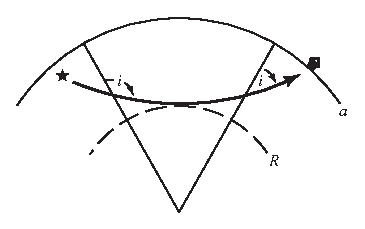
\includegraphics{../figures/chap12/fig01.eps}
\end{center}
\caption[rayparameter]{\label{12.fig.ray}
从源点(星号)到接收点(狗舍)的一条折返射线,其下行段入射角范围为
~$\pi\geq i\geq\pi/2$,上行段为~$\pi/2\geq i\geq 0$。}
\end{figure}
沿射线下行或上行段,波传播方向的单位慢度矢量为
\index{slowness vector}%
\eq
\bph=\brh\cos i+\bThetah\sin i,
\en
其中~$r$、$\Theta$、$\Phi$~为震中球极坐标系的坐标。在地球中任意两点之间,$r$、
$i$~和~$v$~这三个量都在变化;而{\em 射线参数\/}
\index{ray parameter}%
\eq \label{12.pdef}
p=\frac{r\sin i}{v}
\en
则为沿射线的一个常数。因此,从源点出发的不同射线可以用它们的射线参数来做识别或区分。一条射线参数为~$p$~的射线路径可以通过求解如下三个一阶方程得到
\eq \label{12.raytrace}
\frac{dr}{ds}=\cos i,\qquad
\frac{d\Theta}{ds}=r^{-1}\sin i,\qquad
\frac{di}{ds}=pr^{-1}(\dot{v}-v/r).
\en
从~(\ref{12.raytrace}) 中消去作为独立变量的沿射线的路径长度
$s$,可以得到一对耦合的方程组
\eq \label{12.raytrace2}
\frac{dr}{d\Theta}=r\cot i,\qquad
\frac{di}{d\Theta}=r(\dot{v}/v)-1,
\en
利用初始条件~$r(0)=r'$~和~$i(0)=i'$,可以将该方程组做数值积分得到~$r(\Theta)$~和 ~$i(\Theta)$,这里撇号表示在源点位置~$\bx'$~取值。由于在射线的{\em 折返点\/}即最小半径~$R$ ~处,
\index{turning point}%
入射角为~$i=\pi/2$,固~$dr\hspace{-0.4 mm}/\hspace{-0.4 mm}d\Theta=0$,因而射线参数化简为 $p=R/v(R)$。无论何时,如果有必要区分~P、S、K、I~和~J~波的折返点,我们将分别用~$R_{\rm P}$、$R_{\rm S}$、$R_{\rm K}$、$R_{\rm I}$~和~$R_{\rm J}$~来表示。

{\em Benndorf关系\/}将射线参数~$p$~与射线的走时~$T$~及其走过的角距离~$\Theta$~联系起来:
\index{Benndorf's relation}%
\eq \label{12.pdef2}
p=\frac{dT}{d\Theta}.
\en
(\ref{12.pdef2})~表明~$p$~为{\em 角向慢度\/},
\index{slowness!angular}%
\index{angular slowness}%
即走时曲线的斜率。在传播方向上的总慢度为 ~$v^{-1}$,因此一个地震波无论在射线的上行或下行段其{\em 径向慢度\/}的大小均为
\index{slowness!radial}%
\index{radial slowness}%
\eq \label{12.slowness}
q=\sqrt{v^{-2}-p^2r^{-2}}.
\en
对于角频率~$\om>0$~的波,在折返半径~$r=R$ ~以下的瞬逝波区域,我们在~(\ref{12.slowness})~的平方根中选择
~$\Im{\rm m}\,q\geq 0$~的分枝切割。在有必要明确的地方,我们将用带有脚标的符号
~$q_{\alpha}$~和~$q_{\beta}$~来区分压缩波和剪切波的径向慢度。
\index{ray parameter|)}%

\subsection{走时和距离}
\index{travel time|(}%

$T$~和~$\Theta$~这两个量可以通过将微分走时
~$d\hspace{0.2 mm}T=v^{-1}ds$~和角距离
~$d\Theta=r^{-1}\sin i\,ds$~沿相应的射线路径积分得到。
对于射线两端均位于地球表面这一最简单的情形,我们有
\eq \label{12.DistT}
T=2\int_R^a\frac{v^{-2}}{q}\,dr,\qquad
\Theta=2\int_R^a\frac{pr^{-2}}{q}\,dr,
\en
其中因子~2~是为了包括射线的下行和上行两段。
对于反射波如~ScS~或~PKiKP,积分的下限~$R$~需要用
~$b$~或~$c$~取代。对于包含多次反射以及掩埋在地表以下的源点或接收点的更复杂情形,也可以很容易地通过对相应的射线段改变积分上限~$a$,再合并所有积分来处理。

(\ref{12.DistT})~及其推广形式以射线参数~$p$~的函数形式给定了走时
~$T(p)$~和角距离~$\Theta(p)$;这两个关系又以参数形式定义了相关的走时曲线
~$T(\Theta)$。通过考虑~$d\hspace{0.2 mm}T\hspace{-0.5 mm}/\hspace{-0.3 mm}dp$
~和~$d\Theta\hspace{-0.3 mm}/\hspace{-0.3 mm}dp$~这两个导数之间的比值可以证明
Benndorf关系~(\ref{12.pdef2})。
\begin{figure}[!b]
\begin{center}
\scalebox{1.04}{
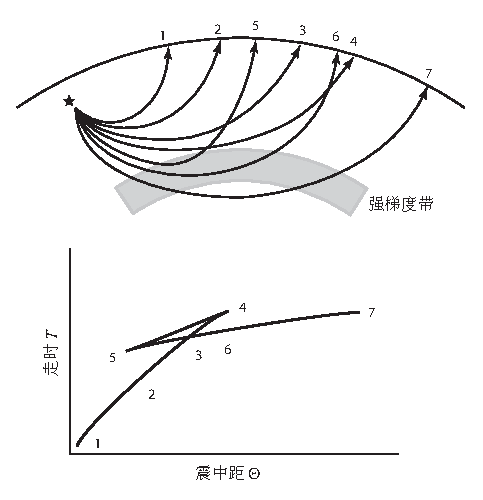
\includegraphics{../figures/chap12/fig02.eps}
}
\end{center}
\caption[triplication]{\label{12.fig.raytrip}
由较强的波速梯度~$\dot{v}<0$~导致的走时曲线三重化示意图。
({\em 上图\/})~射线~1~至~7~具有单调下降的射线参数,即
~$p_1>\cdots >p_7$;震中距~$\Theta(p)$~为一光滑但多值函数。
({\em 下图\/})~相应的走时曲线~$T(\Theta)$;位于~$\Theta_4$~和~$\Theta_5$ 之间的接收点均有三条射线的理论到时。}
\end{figure}
为简单起见,我们假定在软流圈中压缩波与剪切波速度随深度均没有很强的减小,即在地球模型中任何地方均有~$\dot{v} < v/r$。这样,~(\ref{12.raytrace2})~式保证了~$di\hspace{-0.2 mm}/\hspace{-0.4 mm}d\Theta <0$,因而在地幔
~$b\leq r\leq a$~中所有半径上都有一条射线折返,{\em 不存在阴影区\/};
\index{shadow zone}%
任何足够陡的速度随深度的增加,如同在上地幔过渡带中可能会有的那种,都会导致走时曲线的折叠即{\em 三重化\/},如图~\ref{12.fig.raytrip}所示。
\index{triplication}%
走时曲线的尖端会带来焦散现象;沿晚到分支的第三个到达的波经过了焦散区,而前两个到达的波则没有经过(见第12.1.8节)。
\index{travel time|)}%

\subsection{截距时间}
\index{intercept time|(}%

如图~\ref{12.fig.taup}所示,走时曲线的切线在垂直轴上的截距是
\eq \label{12.taudef}
\tau=T-p\Theta,
\en
\begin{figure}[!b]
\begin{center}
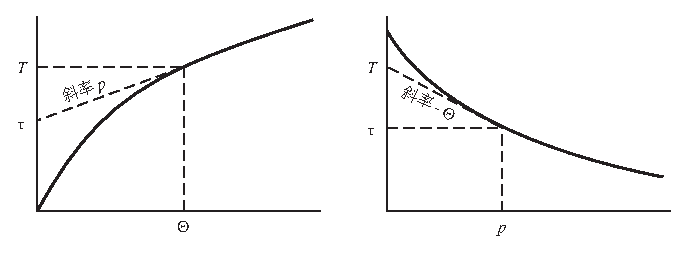
\includegraphics{../figures/chap12/fig03.eps}
\end{center}
\caption[intercepttime]{\label{12.fig.taup}
({\em 左图\/}) $T$ 随 $\Theta$ 的变化曲线与截距时间 $\tau$ 的示意图。 ({\em 右图\/}) 相应的 $\tau$ 随射线参数 $p$ 的变化。两条曲线的导数分别为
$dT/d\Theta=p$ 和 $d\tau/dp=-\Theta$。}
\end{figure}
利用关系式~(\ref{12.DistT}),我们发现该{\em 截距时间\/}是径向慢度的积分:
\index{intercept time}%
\eq \label{12.taudef2}
\tau=2\int_R^aq\,dr.
\en
值得注意的是,在 $\tau$ 的这个积分公式中,走时 $T$ 和震中距 $\Theta$ 所特有的折返点处的 $q^{-1}$ 奇异性被消除了。
对于反射波或者起点与终点不在地球表面的波,需要改变~(\ref{12.taudef2}) 式中的积分限;例如,内核的J波的截距时间是剪切波径向慢度
$q_{\beta}$ 从 $R_{\rm J}$ 到内核边界半径 $c$ 的积分的两倍。

另一个从 $T\hspace{-0.7 mm}-\!\Theta$ 变换到 $\tau\hspace{-0.6 mm}-\!p$ 的优点是它将上地幔三重化“展开了”;截距时间 $\tau$ 始终是随射线参数 $p$ {\em 单调下降\/}的函数,其斜率为
\eq \label{12.tauder}
\frac{d\tau}{dp}=-\Theta.
\en
图~\ref{12.fig.zhao15} 显示了模型1066A
(Gilbert \& Dziewonski \citeyear{gilbert&dziewonski75}) 中所有主要地震波的 $\tau\hspace{-0.6 mm}-\!p$ 曲线。
\begin{figure}[!t]
\begin{center}
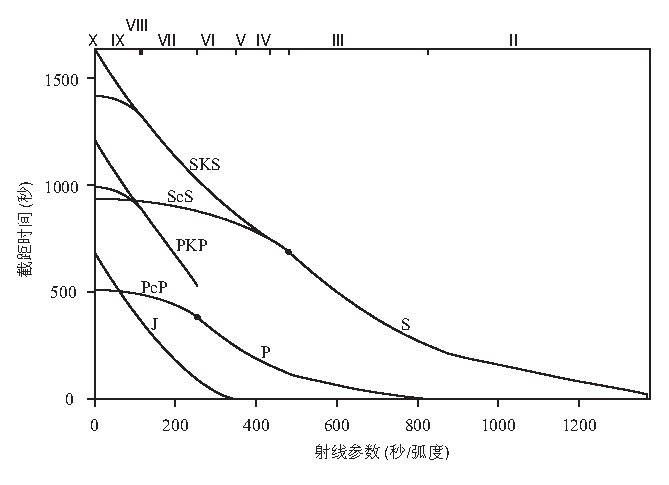
\includegraphics{../figures/chap12/fig04.eps}
\end{center}
\caption[taup1066A]{\label{12.fig.zhao15}
剥去地壳的模型1066A中主要震相的截距时间
$\tau $ 随射线参数 $p$ 的变化曲线。图的顶部标注了P-SV区段II--X。
区段~I 的边界 $p=a/\beta_a$ 位于最右端。曲线上的黑点显示P到PcP 和 S到ScS 变化的拐点。在射线参数较小处,PKP曲线分为({\em 低\/})的PKiKP和({\em 高\/})的PKIKP两个分支;同样地,SKS曲线分为({\em 低\/})的SKiKS和({\em 高\/})SKIKS两个分支。}
\end{figure}
模型中剥去了地壳,并且将地幔的 $\alpha$,$\beta$,$\rho$ 结构参数光滑地外推至地表 $r=a$,从而使模型中只有两个内部不连续面。在下面的讨论中,我们将用带脚标的符号如 $\tau_{\rm P}$ 或 $\tau_{\rm ScS}$ 来区分不同的几何震相。图中并没有显示复合震相如PP或SKKS的曲线;不过,它们的曲线可以很容易地通过将主要震相的曲线相加或相减得到。
\index{intercept time|)}%

\subsection{偏振}
\index{polarization!body-wave|(}%
\index{body-wave polarization|(}%
\label{12.sec.polar}

图~\ref{12.fig.polarization}显示了本书中用来表示P, SV或SH波{\em 质点运动正方向\/}的符号规定。
\index{particle motion!P}%
\index{particle motion!SV}%
\index{polarization!P}%
\index{polarization!SV}%
\begin{figure}
\begin{center}
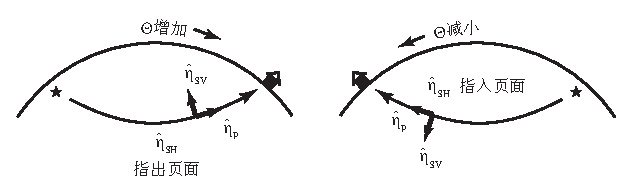
\includegraphics{../figures/chap12/fig05.eps}
\end{center}
\caption[polarizationvectors]{\label{12.fig.polarization}
正确的射线记录方式要求P, SV或SH波的偏振为正的方向
$\hat{\mbox{\boldmath $\eta$}}$ 要有一贯的定义。图中显示的是我们对传播方向为
$\Theta$ 增加 ({\em 左图\/}) 或 $\Theta$ 减小 ({\em 右图\/}) 的射线的定义。}
\end{figure}
一条沿 $\Theta$ 增加方向传播的射线,无论是上行段还是下行段,三种波的偏振矢量均可以显式表示为
\[
\betah_{\rm P}=\brh\cos i+\bThetah\sin i,
\qquad
\betah_{\rm SV}=\brh\sin i-\bThetah\cos i,
\]
\eq \label{12.polar}
\qquad\qquad\qquad\qquad\betah_{\rm SH}=-\bPhih.
\en
对于沿反方向传播的波,所有的偏振矢量均反向,即若 $\Theta\rightarrow -\Theta$,则 $\betah\rightarrow -\betah$,此处 $\betah$
代表 $\betah_{\rm P}$,$\betah_{\rm SV}$,或 $\betah_{\rm SH}$ 中任意一个。普遍的规则是,面向传播方向,压缩波的偏振正方向
$\betah_{\rm P}$ 指向{\em 前方\/},而SV波的偏振正方向 $\betah_{\rm SV}$ 指向{\em 左边\/},SH波的偏振正方向 $\betah_{\rm SH}$ 指向{\em 右边\/}。
\index{polarization!SH}%
\index{polarization!body-wave|)}%
\index{body-wave polarization|)}%

\subsection{反射和透射系数}
\index{reflection coefficient|(}%
\index{transmission coefficient|(}%
\label{12.sec.scatmat}

为了表示平面SH和P-SV波在地球的自由表面以及核幔和内核边界的经典的反射和透射系数,我们对 \textcite{aki&richards80}中所采用的便于记忆的符号做一些变更。在我们的讨论中会用到控制波的{\em 振幅\/}与相应的{\em 能量通量\/}的两种系数;
\index{body-wave amplitude}%
\index{amplitude!body-wave}%
\index{body-wave energy flux}% 
\index{energy flux!body-wave}% 
分别用斜体字母 $P$,$S$,$K$,$I$ 和 $J$ 与草书体字母 $\sP$,$\sS$,$\sK$,$\sI$ 和 $\sJ$ 来表示,同时用抑音与尖音符号来分别表示下行与上行的波传播方向。
SH波入射到自由表面或固-液边界时均发生全反射。此时两种反射系数相等,均为:
$\acute{S}\hspace{-0.4 mm}\grave{S}=
\grave{S}\hspace{-0.4 mm}\acute{S}=
\acute{J}\hspace{-0.5 mm}\grave{J}=
\acute{\sS}\hspace{-0.3 mm}\grave{\sS}=
\grave{\sS}\hspace{-0.3 mm}\acute{\sS}=
\acute{\sJ}\hspace{-0.8 mm}\grave{\sJ}=1$。

在P-SV波的相长干涉分析中,比较方便的做法是用斜体字母系数来表示出射与入射波位移的{\em 径向向上分量\/}的比值
$(\brh\cdot\bs)_{\rm out}/(\brh\cdot\bs)_{\rm inc}$
作为反射与折射系数,而不是用 \textcite{aki&richards80}中的整个位移矢量的振幅比。在地球的自由表面,P-SV波的径向分量的反射系数的表达式为
\eq \label{12.coef1}
\acute{P}\hspace{-0.4 mm}\grave{P}=
\frac{-4p^2a^{-2}q_{\alpha}(a)q_{\beta}(a)
+(\beta_a^{-2}-2p^2a^{-2})^2}
{4p^2a^{-2}q_{\alpha}(a)q_{\beta}(a)+(\beta_a^{-2}-2p^2a^{-2})^2},
\en
\eq
\acute{S}\hspace{-0.4 mm}\grave{P}=\frac{4(\beta_a^{-2}-2p^2a^{-2})
q_{\alpha}(a)q_{\beta}(a)}
{4p^2a^{-2}q_{\alpha}(a)q_{\beta}(a)+(\beta_a^{-2}-2p^2a^{-2})^2},
\en
\eq
\acute{P}\hspace{-0.4 mm}\grave{S}=\frac{4(\beta_a^{-2}-2p^2a^{-2})p^2a^{-2}}
{4p^2a^{-2}q_{\alpha}(a)q_{\beta}(a)+(\beta_a^{-2}-2p^2a^{-2})^2},
\en
\eq \label{12.coef4}
\acute{S}\hspace{-0.4 mm}\grave{S}=\frac{4p^2a^{-2}q_{\alpha}(a)q_{\beta}(a)
-(\beta_a^{-2}-2p^2a^{-2})^2}
{4p^2a^{-2}q_{\alpha}(a)q_{\beta}(a)+(\beta_a^{-2}-2p^2a^{-2})^2},
\en
其中 $p=a\sin i_{\rm P}/\alpha_a=a\sin i_{\rm S}/\beta_a$ 为射线参数。
(\ref{12.coef1})--(\ref{12.coef4}) 中的四个系数满足对称关系
\eq \label{12.coef5}
\acute{P}\hspace{-0.4 mm}\grave{P}=-\acute{S}\hspace{-0.4 mm}\grave{S},
\qquad\acute{P}\hspace{-0.4 mm}\grave{P}\,\acute{S}\hspace{-0.4 mm}\grave{S}
-\acute{P}\hspace{-0.4 mm}\grave{S}\,\acute{S}\hspace{-0.4 mm}\grave{P}=-1.
\en
P-SV波在核幔边界和内核边界的反射与透射系数与此类似,但更为复杂,\textcite{zhao&dahlen93}给出了它们的表达式。

P-SV体波的格林张量用草书体字母形式的反射与透射系数可以更方便地表示,这些系数是{\em 带正负号的\/}的动能加势能的平方根的比值,即
$[|\rho v\cos i|^{1/2}(\betah\cdot\bs)]_{\rm out}
/[|\rho v\cos i|^{1/2}(\betah\cdot\bs)]_{\rm inc}$。
P波的偏振正方向矢量 $\betah$ 总是指向传播方向,而入射与出射的SV波的偏振正方向均指向左侧,如图~\ref{12.fig.zhaoA1}所示。这种正负号的选择与折返射线所采用的一致,但与
\textcite{aki&richards80}所使用的相应规则有所不同。在自由表面 $r=a$ 处,
(能量$)^{1/2}$ 的系数为
\eq \label{12.coef6}
\acute{\sP}\grave{\sP}=
\acute{\sS}\hspace{-0.1 mm}\grave{\sS}=
\frac{4p^2a^{-2}q_{\alpha}(a)q_{\beta}(a)
-(\beta_a^{-2}-2p^2a^{-2})^2}
{4p^2a^{-2}q_{\alpha}(a)q_{\beta}(a)+(\beta_a^{-2}-2p^2a^{-2})^2},
\en
\eq \label{12.coef7}
\acute{\sP}\hspace{-0.3 mm}\grave{\sS}=
-\acute{\sS}\grave{\sP}=
\frac{4(\beta_a^{-2}-2p^2a^{-2})^2pa^{-1}
\sqrt{q_{\alpha}(a)q_{\beta}(a)}}
{4p^2a^{-2}q_{\alpha}(a)q_{\beta}(a)+(\beta_a^{-2}-2p^2a^{-2})^2}.
\en
\begin{figure}[!t]
\begin{center}
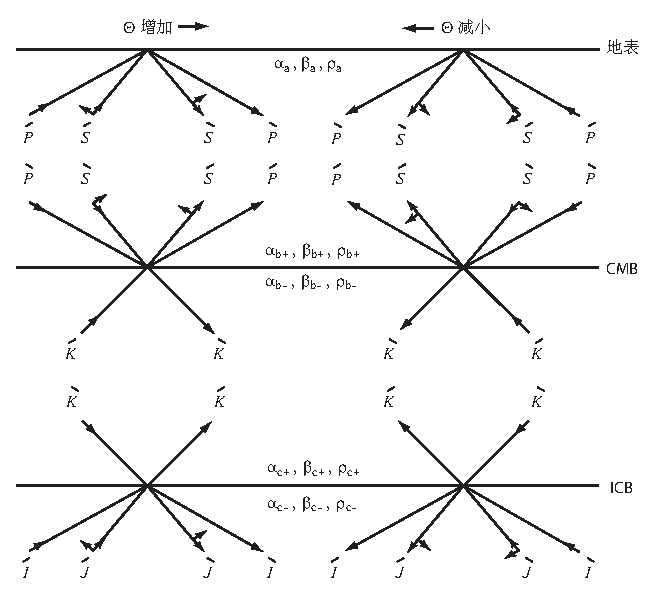
\includegraphics{../figures/chap12/fig06.eps}
\end{center}
\caption[RandTcoeffs]{\label{12.fig.zhaoA1}
表示P-SV波在自由表面、核幔边界(CMB)和内核边界(ICB)的反射和透射系数所使用符号的示意图。正体与斜体字母表示的系数均遵循这些规则。所有入射与出射的P,SV,K, I和J波的偏振正方向 $\hat{\mbox{\boldmath $\eta$}}$ 均由图中箭头指明。}
\end{figure}
(\ref{12.coef6})--(\ref{12.coef7}) 适用于沿 $\Theta$ 增加方向传播的波;对于沿反方向传播的波 $\acute{\sP}\grave{\sP}$
和 $\acute{\sS}\hspace{-0.1 mm}\grave{\sS}$ 不变,
但 $\acute{\sP}\hspace{-0.3 mm}\grave{\sS}$ 和  $\acute{\sS}\grave{\sP}$
会变号。如果我们把这些系数排列成正向与反向的{\em 散射矩阵\/}
\index{scattering matrix}%
\index{matrix!scattering}%
\eq \label{12.scatmat}
\ssS_{\pm}=\left(\begin{array}{rr}
\acute{\sP}\grave{\sP} & \pm\acute{\sP}\hspace{-0.3 mm}\grave{\sS} \\
\pm\acute{\sS}\grave{\sP} & \acute{\sS}\hspace{-0.1 mm}\grave{\sS}
\end{array}\right),
\en
那么这种方向与正负号的变换可以写成简洁的形式
\eq \label{12.scatsym}
\ssS_-=\ssS_+^{\rm T},\qquad\ssS_+=\ssS_-^{\rm T},
\en
其中加号和减号角标表示角度传播方向。很容易验证正向与反向散射矩阵在下式的意义上互为逆矩阵
\eq \label{12.scatsym2}
\ssS_+\ssS_-=\ssS_-\ssS_+=\ssI.
\en
(\ref{12.scatsym2}) 式表达的是在地表的: {\em 入射与出射能量的守恒\/}:
\index{body-wave energy conservation}%
\index{conservation!of body-wave energy}%
\eq
\acute{\sP}\grave{\sP}^{\raise-.5ex\hbox{$\scriptstyle 2$}}
+\acute{\sP}\hspace{-0.3 mm}\grave{\sS}^
{\raise-.5ex\hbox{$\scriptstyle 2$}}=
\acute{\sS}\hspace{-0.2 mm}\grave{\sS}^
{\raise-.5ex\hbox{$\scriptstyle 2$}}+\acute{\sS}\grave{\sP}^
{\raise-.5ex\hbox{$\scriptstyle 2$}}=1.
\en
在核幔边界,P-SV的能量分配满足与~(\ref{12.scatmat}) 类似的一对 $3\times 3$ 散射矩阵:
\eq \label{12.scatmat2}
\ssS_{\pm}=\left(\begin{array}{rrr}
\grave{\sP}\acute{\sP} & \pm\grave{\sP}\hspace{-0.3 mm}\acute{\sS}
& \grave{\sP}\hspace{-0.1 mm}\grave{\sK} \\
\pm\grave{\sS}\acute{\sP} & \grave{\sS}\hspace{-0.1 mm}\acute{\sS}
& \pm\grave{\sS}\hspace{-0.2 mm}\grave{\sK} \\
\acute{\sK}\hspace{-0.1 mm}\acute{\sP} & \pm\acute{\sK}\acute{\sS}
& \acute{\sK}\grave{\sK} \\
\end{array}\right).
\en
在内核边界相应的矩阵为
\eq \label{12.scatmat3}
\ssS_{\pm}=\left(\begin{array}{rrr}
\grave{\sK}\acute{\sK} & \grave{\sK}\grave{\sI}
& \pm\grave{\sK}\hspace{-0.1 mm}\grave{\sJ} \\
\acute{\sI}\hspace{-0.1 mm}\acute{\sK} & \acute{\sI}\grave{\sI}
& \pm\acute{\sI}\hspace{-0.3 mm}\grave{\sJ} \\
\pm\acute{\sJ}\hspace{-0.3 mm}\acute{\sK} &
\pm\acute{\sJ}\hspace{-0.1 mm}\grave{\sI}
& \acute{\sJ}\hspace{-0.8 mm}\grave{\sJ} \\
\end{array}\right).
\en
在一个固-固界面,一个入射SH波会产生一个反射和一个透射波,而一个P或SV波则会产生四个出射波。将P-SV和SH的结果合并在一起,我们可以把全部的能量分配表示成一个 $6\times 6$ 的散射矩阵
\eq \label{12.needin15}
\ssS_{\pm}=\left(\begin{array}{cc}
\ssS_{\pm}^{\rm P\mbox{\scriptsize -}SV} & \sszero \\
\vspace{-1.0 ex} & \vspace{-1.0 ex} \\
\sszero & \ssS_{\pm}^{\rm SH}
\end{array}\right),
\en
其中 $\ssS_{\pm}^{\rm P\mbox{\scriptsize -}SV}$ 和 $\ssS_{\pm}^{\rm SH}$
分别为 $4\times 4$ 和 $2\times 2$ 矩阵。自由表面与固-液界面的散射矩阵~(\ref{12.scatmat})
和~(\ref{12.scatmat2})--(\ref{12.scatmat3}) 也可以扩充为相应的P-SV加SH系统的矩阵,只要将其亚矩阵
$\ssS_{\pm}^{\rm P\mbox{\scriptsize -}SV}$
和 $\ssS_{\pm}^{\rm SH}=\ssI$ 适当地用0和1做填充。每一对正向与反向 $6\times 6$ 散射矩阵 $\ssS_{\pm}$ 均满足~(\ref{12.scatsym})--(\ref{12.scatsym2}) 这两个动力学对称关系。\textcite{kennett83}对形如~(\ref{12.needin15}) 的界面的以及更普遍的弹性散射矩阵的特性做了全面的分析。他所选择的归一化条件是为了便于用反射率方法计算体波的合成地震图,与我们这里使用的不同。在我们的几何约定中,所有的波在折返或反射时均“携带”其偏振信息,这一做法更适用于射线理论的计算。
\index{reflection coefficient|)}%
\index{transmission coefficient|)}%

\subsection{几何扩散}
\index{geometrical spreading!body waves|(}%
\label{12.sec.spread}

在地球的主要不连续面之间的光滑区域,高频地震波的振幅变化受到环绕其相关射线的所谓{\em 射线束\/}的聚焦与散焦的控制。一个时变的P, SV或SH波的能量通量是 $\bK=\om^2\rho v A^2\bph$,其中 $A$ 是频率域位移的振幅。
考虑一条从位于 $\bx'$ 的源点出发的射线,后续相继经过
$\bx_1$ 和 $\bx_2$两点,如图~\ref{12.fig.raytube}所示。
\begin{figure}
\begin{center}
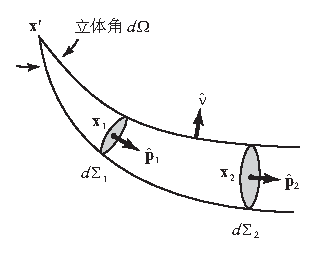
\includegraphics{../figures/chap12/fig07.eps}
\end{center}
\caption[raytubecartoon]{\label{12.fig.raytube}
一个在源点 ${\bf x}'$ 处张开微分立体角 $d\/\Omega$ 的射线束的示意图。在
${\bf x}_1$ 和 ${\bf x}_2$ 两点的单位慢度矢量分别为 $\hat{\bf p}_1$ 和 $\hat{\bf p}_2$,微分截面面积分别为
$d\/\Sigma_1$ 和 $d\/\Sigma_2$。}
\end{figure}
在没有非弹性耗散的情形下,能量守恒要求
$\|\bK\|_1\,d\Sigma_1
=\|\bK\|_2\,d\Sigma_2$,其中 $d\/\Sigma$ 为周围射线束的微分截面面积;
在 $\bx_1$ 和 $\bx_2$ 两点波的振幅之间的关系为
\eq \label{12.ampratio}
\frac{A_2}{A_1}=\left(\frac{\rho_2v_2}
{\rho_1v_1}\right)^{-1/2}\left|\frac{d\Sigma_2}
{d\Sigma_1}\right|^{-1/2}.
\en
绝对值的引入是为了将振幅变化规律~(\ref{12.ampratio}) 推广到射线通过一个或多个焦散区的情形见(第~12.1.8)。

为方便起见,我们可以定义一个类似于均匀介质中的源点-接收点距离 $\|\bx-\bx'\|$ 的量,称为点源的{\em 几何扩散因子\/} $\sR(\bx,\bx')$
\index{geometrical spreading factor}% 
\eq \label{12.Rcodef}
\sR=\sqrt{|d\/\Sigma|/d\Omega},
\en
其中 $d\Omega$ 是射线束在源点 $\bx'$ 处张开的微分立体角,$\bx$ 表示
$\bx_1$ 或 $\bx_2$ 中的任意一个。将~(\ref{12.ampratio}) 中的比值用该因子表示,我们得到完全弹性地球中高频P, SV和SH波的振幅所满足的几何变化规律:
\eq \label{12.amprule}
A\sim(\rho v)^{-1/2}\sR^{-1}.
\en
(\ref{12.amprule}) 式中的符号 $\sim$ 的意思是“沿射线的变化为”。

要计算 $\sR$,我们将在源点 $\bx'$ 处所张开的微分立体角写为
$d\Omega=\sin i'\,|di'|\,d\Phi=
r^{\prime -2}v'q^{\prime -1}p\,|dp|\, d\Phi$,将接收点 $\bx$ 处射线束的微分截面面积写为
$d\/\Sigma=r^2|\!\cos i|\,\sin\Theta\,|d\Theta|\,d\Phi=
r^2vq\sin\Theta\,|d\Theta|\,d\Phi$,其中
$d\Phi$ 为在与射线平面垂直方向上的微分方位角。利用这些表达式以及
~(\ref{12.tauder}) 式,我们得到
\eq \label{12.Rcoef}
v'\sR=rr'\sqrt{\frac{vv'qq'\sin\Theta}{p}
\left|\frac{d^2\tau}{dp^2}\right|}.
\en
从~(\ref{12.Rcoef}) 的形式可以明显看出每一条简单或复合射线的扩散系数都满足动力学的{\em 互易关系\/}
\index{reciprocity!geometrical spreading factor}%
\eq \label{12.Rcoef2}
v(\bx')\sR(\bx,\bx')=v(\bx)\sR(\bx',\bx).
\en
(\ref{12.Rcoef})--(\ref{12.Rcoef2}) 这两个结果不仅适用于直达的P波和S波,也适用于所有串接起来的复合波,如PcP和SKKS,无论经过多少次反射,折射和转换;方向余弦的绝对值 
$v'q'=|\!\cos i'|$ 和 $vq=|\!\cos i|$ 分别属于离开
$\bx'$ 和到达 $\bx$的波,即使在中途波的类型发生了改变,如PS或ScP。
图~\ref{12.fig.zhao15} 显示~(\ref{12.Rcoef}) 中的曲率
$d^2\tau/dp^2$ 对于如P,S,PKP和SKS所有这些折返波都是正的,而对于如PcP,ScS,PKiKP和SKiKS所有这些反射波则都是负的。

对于一个固定的源点 $\bx'$,几何扩散因子
$\sR(\bx,\bx')$ 是沿射线上接收点位置 $\bx$ 的连续函数,仅在内部界面处有一个不连续的跃变。
乘积 $\sR\,|\cos i|^{-1/2}$ 也是连续的;在反射和折射时
$|\cos i|^{-1/2}=(vq)^{-1/2}$ 这个量的跃变引起射线束截面面积的变化。对于复合射线,振幅变化规律
~(\ref{12.amprule}) 可以推广为
\eq \label{12.amprule2}
A\sim(\rho v)^{-1/2}\Pi\sR^{-1},
\en
其中 $\Pi$ 为沿射线路径上所有 (能量$)^{1/2}$
的反射和透射系数
$\grave{\sP}\hspace{-0.3 mm}\acute{\sS}$,
$\grave{\sP}\hspace{-0.1 mm}\grave{\sK}$,等等的乘积。
(\ref{12.amprule2}) 这一关系确保了从任一无穷小立体角
$d\Omega$ 内离开源点的动能加势能都是守恒的;反射-透射系数的乘积 $\Pi$ 的作用是在每一个界面处将入射波能量分配给各个出射波。
\index{geometrical spreading!body waves|)}%

\subsection{焦散相移}
\index{caustic phase shift|(}%
\index{phase shift!caustic|(}%

在~(\ref{12.ampratio})
和~(\ref{12.Rcodef}) 两式中必须用绝对值来处理可能的{\em 焦散现象\/},
\index{caustic}%
即射线束的微分截面面积 $d\/\Sigma$ 变为零的情形,如图~12.8所示。
每当一个波通过一个线状焦散,它会有一个
$\pi/2$ 的非几何的相位提前。为方便记忆,我们可以把这一现象看作是由于~(\ref{11.piover2})式中射线束的面积改变了符号:
\begin{figure}[!b]
\centering
\begin{tabular}{lr}
\begin{tabular}{l}
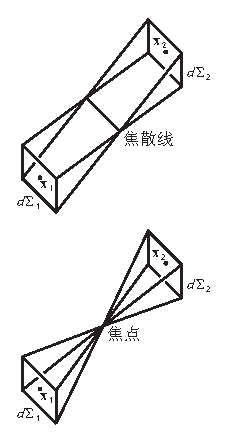
\includegraphics{../figures/chap12/fig08.eps}
\end{tabular}
&
\hspace{1.5cm}
\parbox{4.5cm}{\small
\vspace{1.5cm}
Figure 12.8. ({\em 上图\/}) 对于一个线状焦散,射线束的截面面积仅在一个横向的方向变为零。如果
$d\/\Sigma_1$ 在 ${\bf x}_1$ 为正,则 $d\/\Sigma_2$ 在 ${\bf x}_2$ 可看作为负。({\em 下图\/}) 对于点状焦散,射线束在两个横向的方向同时“跌落”为零(此处波的相位提前为
$\pi$ 而不是 $\pi/2$) ,这种情形在SNREI地球模型中极为罕见。\vspace{2.0cm}}
\end{tabular}
\end{figure}
\addtocounter{figure}{1}
\eq \label{12.over2}
\left(\frac{d\/\Sigma_2}{d\/\Sigma_1}\right)^{1/2}=\;
\left|\frac{d\/\Sigma_2}{d\/\Sigma_1}\right|^{1/2}
\exp(i\pi/2).
\en
Landau \& Lifshitz (\citeyear{landau&lifshitz71}) 对通过线状焦散的
$\pi/2$ 位提前做了严格的波动理论推导。在~(\ref{12.amprule2}) 中引入焦散相移,我们得到射线理论体波振幅变化规律的最终形式:
\eq \label{12.amprule3}
A\sim(\rho v)^{-1/2}\Pi\sR^{-1}\exp(iM\pi/2).
\en
其中整数 $M$ 是所谓的 {\em Maslov 指数\/},
\index{Maslov index}%
\index{index!Maslov}%
它追踪通过线状焦散的次数。通常射线每通过一个线状焦散
$M$ 就加1;在通过比较罕见的点状焦散时,$M$ 要加2。每一条射线所通过的线状或点状焦散的次数与其反向射线是相等的:
\eq \label{12.Maslovsymm}
M(\bx,\bx')=M(\bx',\bx).
\en
例如,SS与其反向传播的射线均在它们的第二个折返点处通过唯一的线状焦散。
\index{reciprocity!Maslov index}%
\index{Maslov reciprocity principle}%
\index{caustic phase shift|)}%
\index{phase shift!caustic|)}%
\index{ray theory!body-wave|)}%
\index{body-wave ray theory!SNREI Earth|)}%

\section{相长干涉原理}
\index{constructive-interference principle|(}%

SNREI地球中的自由振荡是以{\em 相同射线参数\/} $p$ 传播的SH 和 P-SV体波的相长干涉而产生的驻波。在本节中,我们基于这一思想,用基本的物理观念来推导SNREI地球模型中简正模式本征频率的渐近公式。这里所提到的内容可以在原始文献
Brune (\citeyear{brune64}; \citeyear{brune66}), \textcite{odaka78},
\textcite{levshin81} 和 \textcite{zhao&dahlen93}中找到逐步完善的描述。由于傅里叶变换的定义上的差别,这里所用到的所有波的相位均与\textcite{zhao&dahlen93}中的符号相反。

\subsection{Jeans关系}
\index{Jeans relation|(}%

图~\ref{12.fig.2caustics}的左图中显示了一个具有相同射线参数 $p$ 的折返射线家族。
\begin{figure}[!b]
\begin{center}
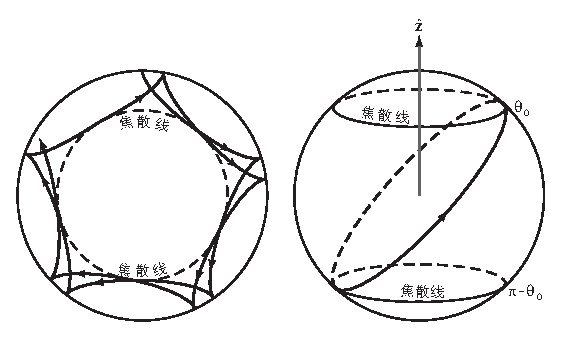
\includegraphics{../figures/chap12/fig09.eps}
\end{center}
\caption[JeansRelation]{\label{12.fig.2caustics}
({\em 左图\/}) 地球大圆截面示意图,显示一个具有相同射线参数 $p$ 的折返射线家族形成的圆形焦散。 ({\em 右图\/}) 一个在南北半球余纬度 $\theta_0$ 和 $\pi-\theta_0$ 折返的射线家族形成的圆锥口焦散。}
\end{figure}
每一条射线都在相同的半径折返;因而半径为 $R$ 的圆成为这些射线的包络线,即 {\em 焦散\/}。
\index{caustic}%
如果我们假定所有射线与 $\bzh$ 轴形成的倾角也相同,那么也会有与北半球和南半球的两个折返余纬度相应的圆锥口焦散,如图~\ref{12.fig.2caustics}中的右图所示。
从本质上讲,寻求地球的渐近简正模式的问题是一个{\em 量子化\/}问题---相长干涉所要求的是在球面上以及在 $r=R$ 和 $r=a$ 这两个半径之间必须能够正好“装下”整数个振荡。确保这一结果的条件类似于准经典量子力学中的{\em 玻尔-索末菲\/}量子化条件
(Born \citeyear{born27};
Landau \& Lifshitz \citeyear{landau&lifshitz65})。
\index{Bohr-Sommerfeld quantization}%
由于目前涉及的是三维几何,所以有三个独立的量子化条件,以及三个独立的量子数;在本节的剩余部分,我们考虑其中最简单的---角度量子化。

与图~\ref{12.fig.2caustics}所示射线家族相应的波或相位波前的传播角速度为
$d\Theta\hspace{-0.3 mm}/\hspace{-0.3 mm}dT=p^{-1}$;与此相应,一个角频率为 $\omega$ 的波所感受到的相位的空间变化率为
$\omega(dT/d\Theta)=\omega p$。在走过地球一整圈之后,
即 $\Theta\rightarrow\Theta+2\pi$,这个波的总的相位累积为
\eq \label{12.Bohr1}
\Delta\Psi=-2\pi\omega p+\pi,
\en
其中等号右边第一项的负号取决于我们使用的傅里叶变换定义,第二项则是由于通过北半球和南半球的焦散而产生的两个 $\pi/2$ 相移。这一行波的玻尔-索末菲相长干涉条件为
\eq \label{12.Bohr2}
|\Delta\Psi|=2\pi l,
\en
其中 $l$ 为一非负整数。将~(\ref{12.Bohr1}) 与~(\ref{12.Bohr2}) 比较,可以得到著名的角度量子化关系
\eq \label{12.Jeans}
\omega p=l+\half.
\en
我们将会看到,量子数 $l$ 是模式 ${}_n{\rm T}_l$ 或 ${}_n{\rm S}_l$ 的
{\em 角级数\/}。(\ref{12.Jeans}) 式对任何的 $l$ 值都成立,包括 $l=0$,这一结果是\textcite{jeans23}在关于地震波在一个球内传播的经典研究中首次得到的。

在短波极限, $l\gg 1$,Jeans关系与附录~B.7中得到的 $m\geq 0$ 阶的表面球谐函数的渐近表达式一致:
\eqa \label{12.Ylm1}
\lefteqn{X_{lm}(\theta)\approx\frac{1}{\pi}
(\sin^2\theta-\sin^2\theta_0)^{-1/4}} \nonumber \\
&&\mbox{}\times\cos\left[(l+\half)\arccos(\cos\theta/\!\cos\theta_0)
\right. \nonumber \\
&&\qquad\mbox{}-\left.m\arccos(\cot\theta/\!\cot\theta_0)
+m\pi-\fourth\pi\right],
\ena
其中
\eq \label{12.Ylm2}
\theta_0=\arcsin\left(\frac{m}{l+\half}\right).
\en
每一个本征函数形式为
$\sqrt{2}\,X_{lm}(\theta)\cos m\phi$,$X_{l0}(\theta)$ 或
$\sqrt{2}\,X_{lm}(\theta)\sin m\phi$ 
的驻波都是由与 $\bzh$ 轴形成相同倾角的顺时针和逆时针传播的两个波合成得来的,如图
~\ref{12.fig.2caustics}所示。这两个相长干涉的波的局地波数均为半整数:  
\eq
k=\sqrt{l(l+1)}\approx l+\half.
\en
然而,由于两个 $\pi/2$ 焦散相移的存在,在每个与折返余纬度 $\theta_0$ 和 $\pi-\theta_0$ 相切的大圆上有整数个振荡—恰好 $l$ 个。在早期的量子力学中,人们已经注意到当量子数为半整数而不是整数时,理论与观测常常会更吻合,但是并没有任何理论依据来确定究竟是半整数还是整数更合理。这一缺陷直到旧的理论被现代量子力学取代了很久以后才得到纠正,是 \textcite{keller58}和 \textcite{keller&rubinow60}证明了这个问题可以通过计算经典轨道的过焦散的次数来解决。

(\ref{12.Ylm2}) 式可以被看作是在 $\theta_0$ 和 $\pi-\theta_0$ 这两个折返余纬度之间容纳 $l-m$ 个振荡的玻尔-索末菲条件。第二个角量子数 $m$ 当然是围绕任一纬度线的 $0\leq \phi\leq 2\pi$ 经度上的振荡个数。这个数被称为振荡的{\em 阶数\/},由于地球模型的球对称性,它在本征频率的渐近分析中不起作用。
Jeans关系~(\ref{12.Jeans}) 为环型和球型振荡的本征频率
${}_n\om_l^{\rm T}$ 和 ${}_n\om_l^{\rm S}$ 提供了一个约束;另一个约束的提供者---径向量子化条件---正是问题的关键所在。
\index{Jeans relation|)}%

\subsection{环型模式}
\index{mode-ray duality!toroidal modes|(}%
\label{12.sec.TOR}

我们首先考虑因地幔中折返的SH波的相长干涉而产生的环型模式这一例子;这些波的射线参数的范围是 $b/\beta_{b+}<p<a/\beta_a$。图~\ref{12.fig.zhao1}的左图显示了这种 ${\rm SSS}\cdots$ 波的射线路径在地球表面 $r=a$ 上A和B两点之间的一段。
\begin{figure}
\begin{center}
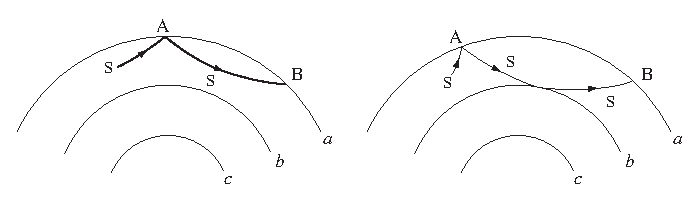
\includegraphics{../figures/chap12/fig10.eps}
\end{center}
\caption[S&ScSFeynman]{\label{12.fig.zhao1}
区段~II中折返SH波 ({\em 左图\/}) 和区段~III中反射 ${\rm ScS}_{\rm SH}$ 波
({\em 右图\/}) 的射线路径示意图。相长干涉分析是对波在B点和A点之间的相位差的量子化。}
\end{figure}
走过该段路径的SH波所累积的相位为
\eq \label{12.Psi1}
\Delta\Psi=-\omega T+\pi/2,
\en
其中 $T(p)$ 为走时,右边第二项表示波在通过折返点产生的焦散相移。要使这一SH波在到达B点时与所有射线参数为 $p$ 的波发生相长干涉,必须有
\eq \label{12.Psi2}
|\Delta\Psi|=\omega p\Theta+2n'\pi,
\en
其中 $\Theta(p)$ 为角距离,$n'$ 为正整数。将~(\ref{12.Psi1}) 与~(\ref{12.Psi2}) 比较,我们看到
\eq \label{12.freq1}
\omega(T-p\Theta)=\omega\tau=2\pi(n'+\fourth),
\en
其中 $\tau(p)$ 为截距时间。习惯上的排序规则是把最低阶的模式称为零阶而不是一阶,为保持一致,我们令 $n'=n+1$。因而玻尔-索末菲径向量子化条件~(\ref{12.freq1}) 的最终形式为
\eq \label{12.freq2}
\omega\tau_{\rm S}=2\pi(n+\fivefourths),
\en
其中 $n$ 为常用的径向阶数,这里我们加上了脚标 S 来提示我们这是与SH等价的模式。

图~\ref{12.fig.zhao1}中右图所示的 ${\rm ScS}_{\rm SH}$ 等价的模式的相长干涉分析可以采用类似的方式。唯一的区别是~(\ref{12.Psi1}) 中的 $\pi/2$ 一项不存在,因为横向偏振的波在固-液边界反射时不产生任何相移。折返波的焦散相移是导致公式~(\ref{12.freq1}) 中的四分之一整数的量子数
$n'+\fourth$ 的原因;取代~(\ref{12.freq2}) 的 ${\rm ScS}_{\rm SH}$ 模式的径向量子化条件为
\eq \label{12.freq3}
\omega\tau_{\rm ScS}=2\pi(n+1).
\en
为消除任何模糊之处,我们再次强调,在SH等价模式中 $\pi/2$ 相移的出现是因为所有相关的波{\em 均具有相同的射线参数\/}。地震或其它点源所激发的折返SH波都具有不同的射线参数;它们没有焦散相移。我们将在第~12.5.1节讨论 ${\rm SS}_{\rm SH}$ 这类有多个射线段的震相的焦散相移。

总体来说,在 $0< p< \infty$ 范围内,SH波有四个不同的射线参数区段;表~\ref{table:SH}中总结了每一个区段上所存在的振荡型的波动及其相应的渐近本征频率方程。内核的 ${\rm J}_{\rm SH}$ 模式的干涉分析与地幔的SH模式完全一样,因为在内核边界的反射是无相移的全反射。此外,还有一个极限射线参数 $p=a/\hspace{-0.2 mm}\beta_a$,在射线参数大于此值时没有任何振荡型波动可以传播;也不存在任何大于此射线参数的渐近环型模式。

\begin{table}[!b]
\centering
\begin{tabular}{|c|c|c|c|} \hline
& & & \\
区段 & 射线参数 & 振荡型体波 & 本征频率 \\
& & & \\ \hline
& & & \\
I & $a/\hspace{-0.2 mm}\beta_a < p<\infty$ & 无 & --- \\
& & & \\
II & $b/\hspace{-0.2 mm}\beta_{b+}<p<a/\hspace{-0.2 mm}\beta_a$ & 折返 SH &
  $\omega\tau_{\rm S}=2\pi(n+\fivefourths)$ \\
& & & \\
III & $0< p<b/\hspace{-0.2 mm}\beta_{b+}$ & ${\rm ScS}_{\rm SH}$ &
  $\omega\tau_{\rm ScS}=2\pi(n+1)$ \\
& & & \\
IV & $0< p<c/\hspace{-0.2 mm}\beta_{c-}$ & 折返 ${\rm J}_{\rm SH}$ &
  $\omega\tau_{\rm J}=2\pi(n+\fivefourths)$ \\
& & & \\ \hline
\end{tabular}
\caption[SH modes]{仅有两个内部不连续面的地球模型中SH波的射线参数区段。每一区段有各自的环型模式渐近本征频率方程。}
\label{table:SH}
\end{table}

图~\ref{12.fig.zhao16}比较了模型1066A的地幔环型模式的渐近与精确的频散曲线图。
\begin{figure}[!t]
\begin{center}
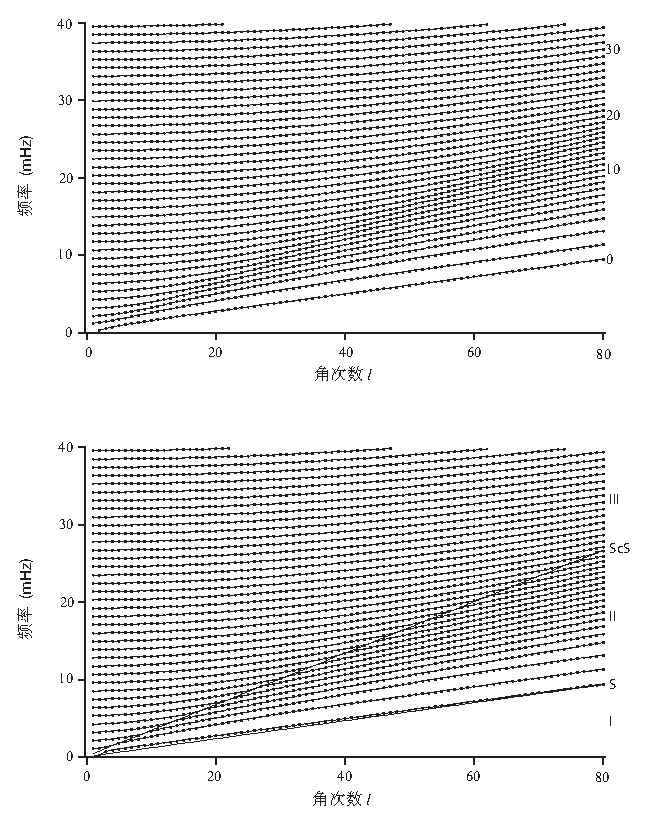
\includegraphics{../figures/chap12/fig11.eps}
\end{center}
\caption[ToroidalDispersion]{\label{12.fig.zhao16}
无地壳的1066A模型的环型模式频散曲线图。
({\em 上图\/}) 用数值积分计算的精确的简并本征频率 ${}_n\omega_l^{\rm T}$。
({\em 下图\/}) 用方程~(\ref{12.freq2})--(\ref{12.freq3}) 计算的渐近本征频率。标有S和ScS的斜线的射线参数分别为 
$p=a/\beta_a$ 和 $p=b/\beta_{b+}$。  (由 L.\ Zhao提供)}
\end{figure}
图中标有S和ScS的粗斜线是射线参数为常数的直线,它们分别是表~\ref{table:SH}中前三个射线参数区段之间的分界线。区段~I和~II之间的边界对应于SH波存在的临界值,而区段~II和~III之间的边界则与掠射地核的射线相同;区段~IV中的 ${\rm J}_{\rm SH}$ 内核模式没有显示。很明显的,渐近与精确的本征频率之间有极好的一致性,甚至包括基阶和最低几阶的分支。从当前的观点来看,这些与勒夫波等价的模式是上地幔折返的SH波相长干涉的结果。每一条 $\omega\!-\!l$ 曲线在 $p=b/\hspace{-0.2 mm}\beta_{b+}$ 处的转折来自于连续的 $\tau\!-\!p$ 曲线中分隔~ScS波与~S波的拐点 (见图~\ref{12.fig.zhao15})。这两幅图的主要差别都出现在这个转折附近;每一条渐近 $\omega\!-\!l$ 曲线在跨过 $p=b/\hspace{-0.2 mm}\beta_{b+}$ 这条线时,都会因 $n+1\rightarrow n+5/4$ 这一量子数跃变 而表现出不连续。这是由几何射线近似而人为造成的,因为几何射线近似只有在无限高频 $\omega\rightarrow\infty$ 时才严格成立。在这条线附近,地核掠射波的隧道效应及其它有限频效应会使频率有限的~SH和 ${\rm ScS}_{\rm SH}$ 两种不同模式变得难以区分。

一些研究者已经探讨过莫霍面和上地幔不连续面的影响;它们的主要作用是造成环型模式 $\omega\!-\!l$ 曲线的些微起伏,类似于球型模式曲线中的那种密切接近和阶梯状的情形,但是要弱很多。这种所谓的{\em 独调效应\/}效应在图~\ref{fig:tormodefreqs}所展示的PREM频散曲线图的分辨尺度上不容易看出来;它只有在仔细检视本征频率的精确数值结果与用渐近关系~(\ref{12.freq2})--(\ref{12.freq3}) 计算的结果之间的差别时才能察觉到。
\index{solotone effect}%
从本质上讲,独调效应是一种与像 S{\scriptsize 410}${\rm S}_{\rm SH}$
和 S{\scriptsize 660}${\rm S}_{\rm SH}$ 这些反射波存在相关的共振现象;
\textcite{lapwood&usami81}概述了相关理论及其原始参考文献。任何企图在像PREM那样接近真实的地球模型中对渐近本征频率做精确计算的定量算法都不仅要考虑各个不连续面的反射波,还要考虑每一个光滑层内接近掠射不连续面的折返射线的隧道效应。如前所述,我们在本章中的目标十分有限:我们仅寻求揭示各种不同类型的SH和P-SV模式的明显的物理特征。除了两个主要的固-液边界之外,更多的不连续面会对定量的细节有影响,但不会改变总的物理图像。

在结束本节之前我们来介绍另外一种推导环型模式本征频率关系的方法,用一种更易于推广到我们下一步要考虑的球型模式的思路。在这一更普遍适用的思路中,我们并不是专注在图~\ref{12.fig.zhao1}所显示的波的相位上,而是它们的复数振幅。首先还是仅考虑SH等价模式,将A点横向分量的振幅用 $a_{\rm S}$ 表示,而B点的振幅可以有两种不同的计算方法:
\begin{enumerate}
\item 因为在球形自由表面上的相位变化速率为
$p^{-1}=d\Theta\hspace{-0.2 mm}/\hspace{-0.2 mm}dT$,
B点的振幅必定是 $a_{\rm S}\exp(-i\omega p\Theta)$。
\item
然而,如果考虑沿折返射线的相位变化,我们得到振幅也必须是
$a_{\rm S}\exp(-i\om T_{\rm S}+i\pi/2)$,其中 $T_{\rm S}$
为SH波走时,
\index{travel time!SH-wave}%
$\pi/2$ 表示焦散相移。因为构成相应射线束的射线
{\em 均有相同的射线参数\/} $p$。
\end{enumerate}
令上述两个结果相等,我们得到B点的相长干涉条件为
\eq \label{12.sanscarr1}
a_{\rm S}\exp(-i\om T_{\rm S}+i\pi/2)=a_{\rm S}\exp(-i\omega p\Theta).
\en
类似的关系也适用于 ${\rm ScS}_{\rm SH}$ 等价模式,只要把
走时 $ T_{\rm S}$ 换成 $T_{\rm ScS}$,
并把相移 $\pi/2$ 改为零:
\eq \label{12.sanscarr2}
a_{\rm S}\exp(-i\om T_{\rm ScS})=a_{\rm S}\exp(-i\omega p\Theta).
\en

归结以上思路的基本要点,我们在~(\ref{12.sanscarr1})--(\ref{12.sanscarr2}) 的两边均除以 $\exp(-i\omega p\Theta)$,便可得到会在后面推广到P-SV情形的SH 和${\rm ScS}_{\rm SH}$ 的相长干涉条件:
\eq \label{12.aeqn1}
a_{\rm S}\exp(-i\Psi_{\rm S})=a_{\rm S},\qquad
a_{\rm S}\exp(-i\Psi_{\rm ScS})=a_{\rm S},
\en
其中我们已经做了如下定义
\eq \label{12.PsiSdef}
\Psi_{\rm S}=\omega\tau_{\rm S}-\pi/2,\qquad
\Psi_{\rm ScS}=\omega\tau_{\rm ScS}.
\en
(\ref{12.aeqn1}) 的左右两边均表示相应的SH和
${\rm ScS}_{\rm SH}$ 波的复数振幅,它们都是相对于一个以均匀角速度 $p^{-1}=d\Theta\hspace{-0.2 mm}/\hspace{-0.2 mm}dT$ 传播的“载波”
$\exp(-i\om p\Theta)$ 而言的。这一相对振幅与{\em 在球面上的位置无关\/},
即在A点和B点相等。消去~(\ref{12.aeqn1}) 中的 $a_{\rm S}$,再利用标准的三角函数等式,我们得到SH和 ${\rm ScS}_{\rm SH}$ 本征频率的一对实数关系式
\eq \label{12.torfreq}
\sin\half\Psi_{\rm S}=0,\qquad
\sin\half\Psi_{\rm ScS}=0,
\en
以上关系式与~(\ref{12.freq2})--(\ref{12.freq3}) 是等价的。
\index{mode-ray duality!toroidal modes|)}%

\subsection{球型模式}
\index{mode-ray duality!spheroidal modes|(}%

对于P-SV波,一个仅有内核边界和核幔边界两个内部不连续面的分段光滑地球模型中有十个独立的射线参数区段。与SH波一样,必须将相长干涉原理分别应用于每一个区段。
表~\ref{table:PSV}列出了对应于边界上临界和掠射射线的区段分界值 $p$ 以及区段内存在的振荡型的波。我们通过讨论区段~III中的地幔球型模式和区段~IX中的 PKIKP,${\rm ScS}_{\rm SV}$ 和 ${\rm J}_{\rm SV}$ 模式来展示使用的分析方法。分析中即可以用垂直分量也可以纵向分量;我们这里采用前者。
\index{particle motion!body-wave}%
\index{polarization!body-wave}%
\index{body-wave polarization}%

\begin{table}[!t]
\centering
\begin{tabular}{|c|c|l|} \hline
& & \\
区段 & 射线参数 & 振荡型体波 \\
& & \\ \hline
& & \\
I & $\,a/\hspace{-0.2 mm}\beta_a<p<\infty$ & 无 \\ 
& & \\
II & $\,a/\hspace{-0.2 mm}\alpha_{a}<p<a/\hspace{-0.2 mm}\beta_a$ & 折返 SV \\
& & \\
III & $b/\hspace{-0.2 mm}\beta_{b+}<p<a/\hspace{-0.2 mm}\alpha_{a}$
& 折返 P 和折返 SV \\ & & \\
IV & $b/\hspace{-0.2 mm}\alpha_{b-}<p<b/\hspace{-0.2 mm}\beta_{b+}$ &
折返 P 和 ${\rm ScS}_{\rm SV}$ \\
& & \\
V & $c/\hspace{-0.2 mm}\beta_{c-}<p<b/\hspace{-0.2 mm}\alpha_{b-}$ &
折返 P,${\rm ScS}_{\rm SV}$ 
   和SKS \\
& & \\
VI & $b/\hspace{-0.2 mm}\alpha_{b+}<p<c/\hspace{-0.2 mm}\beta_{c-}$ &
折返 P,${\rm ScS}_{\rm SV}$,
SKS和 \\
& & 折返 ${\rm J}_{\rm SV}$ \\
& & \\
VII & $c/\hspace{-0.2 mm}\alpha_{c+}<p<b/\hspace{-0.2 mm}\alpha_{b+}$ &
PKP, PcP, PKS, PcS, SKS, \\
& & ${\rm ScS}_{\rm SV}$, SKP, ScP 和 \\
& & 折返 ${\rm J}_{\rm SV}$ \\
& & \\
VIII & $c/\hspace{-0.2 mm}\alpha_{c-}<p<c/\hspace{-0.2 mm}\alpha_{c+}$ &
PKiKP, PKJKP, PcP, PKiKS, \\
& &  PKJKS, PcS, SKiKS, SKJKS, \\
& & ${\rm ScS}_{\rm SV}$, SKiKP, SKJKP 和 ScP \\
& & \\
IX & $0<p<c/\hspace{-0.2 mm}\alpha_{c-}$ & PKIKP, PKJKP, PKiKP, PcP, \\
& &  PKIKS, PKJKS, PKiKS, PcS, \\
& &  SKIKS, SKJKS, SKiKS, ${\rm ScS}_{\rm SV}$, \\
& & SKIKP, SKJKP, SKiKP 和 ScP \\
& & \\
X & $p=0$ (径向模式) & PKIKP, PKiKP 和 PcP \\
& & \\ \hline
\end{tabular}
\caption[SH modes]{仅有两个内部不连续面的地球模型中P-SV波的射线参数区段。区段分界在图~\ref{12.fig.zhao15}中的 $\tau\!-\!p$ 曲线图顶端有所显示。每个区段各有相应的球型模式渐近本征频率方程。核幔边界和内核边界上的~Stoneley 模式分别出现在区段~III和~V。}
\label{table:PSV}
\end{table}

我们分别用 $a_{\rm P}$ 和 $a_{\rm S}$表示区段~III中入射~P和~SV波的径向向上振幅。
参照图~\ref{12.fig.zhao5},我们可以写出B和C两点的相长干涉条件
\eq \label{12.aP1}
(a_{\rm P}\acute{P}\hspace{-0.4 mm}\grave{P}
+a_{\rm S}\acute{S}\hspace{-0.4 mm}\grave{P})
\exp(-i\Psi_{\rm P})=a_{\rm P},
\en
\eq \label{12.aS1}
(a_{\rm P}\acute{P}\hspace{-0.4 mm}\grave{S}
+a_{\rm S}\acute{S}\hspace{-0.4 mm}\grave{S})
\exp(-i\Psi_{\rm S})=a_{\rm S},
\en
其中
\eq \label{12.PsiPdef}
\Psi_{\rm P}=\omega\tau_{\rm P}+\pi/2,\qquad
\Psi_{\rm S}=\omega\tau_{\rm S}-\pi/2.
\en
\begin{figure}[!t]
\begin{center}
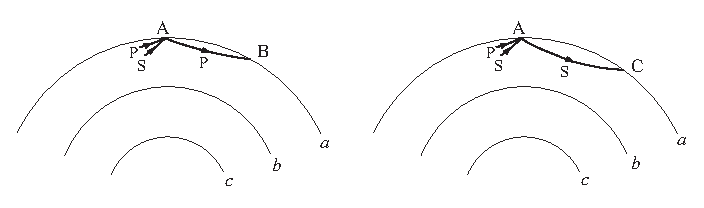
\includegraphics{../figures/chap12/fig12.eps}
\end{center}
\caption[S&PFeynman]{\label{12.fig.zhao5}
区段~III中折返P波和SV波的射线路径示意图。B点的P波和C点的SV波来自两个入射到A点的波结合并与自由表面作用的结果。左右两图中射线的“历程”或“费曼”图分别导致~(\ref{12.aP1}) 和~(\ref{12.aS1}) 两式。}
\end{figure}
(\ref{12.aP1})--(\ref{12.aS1}) 两式左边的部分均可以被视为对两种波所走过的“历程”依时间顺序的描述:在A点入射、结合并与边界发生作用,最终分别到达B和C两点。如~(\ref{12.aeqn1}) 中的SH--${\rm ScS}_{\rm SH}$ 一样,所有振幅都是相对于角向的“载波”
$\exp(-i\om p\Theta)$ 而言的,这一相对振幅在A,B和C三点相等。与第~\ref{12.sec.scatmat}节讨论的一样,自由表面的四个反射系数
$\acute{P}\hspace{-0.4 mm}\grave{P}$,
$\acute{P}\hspace{-0.4 mm}\grave{S}$,
$\acute{S}\hspace{-0.4 mm}\grave{P}$ 和
$\acute{S}\hspace{-0.4 mm}\grave{S}$ 是出射与入射波位移的径向向上分量的比值。
(\ref{12.PsiPdef}) 式所定义的 $\Psi_{\rm P}$ 的第二项包含了P波的
$\pi/2$ 焦散相移及其径向向上分量在通过折返点半径 $r=R_{\rm P}$ 时符号反向的综合效应,如图~\ref{12.fig.zhao6}所示。
\begin{figure}
\begin{center}
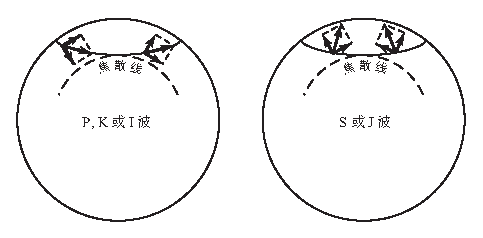
\includegraphics{../figures/chap12/fig13.eps}
\end{center}
\caption[turning sign]{\label{12.fig.zhao6}
P,K和I波的径向分量 ({\em 左图\/})
与SV和 ${\rm J}_{\rm SV}$ 波的切向分量 
({\em 右图\/}) 在折返点处为零。而P,K和I波的切向分量与
SV 和 ${\rm J}_{\rm SV}$ 波的径向分量则有极大值。每一个位移矩形内的对角矢量为偏振矢量
$\hat{\mbox{\boldmath $\eta$}}_{\rm P}$ ({\em 左图\/}) 和
$\hat{\mbox{\boldmath $\eta$}}_{\rm SV}$ ({\em 右图\/})。}
\end{figure}
在SV波通过 $r=R_{\rm S}$ 时,其径向向上分量的符号不变,因此 $\Psi_{\rm S}$ 与~(\ref{12.PsiSdef}) 式给定的折返SH的一样。
(\ref{12.aP1})--(\ref{12.aS1}) 这两个相长干涉条件构成一组关于未知相对振幅
$a_{\rm P}$ 和 $a_{\rm S}$ 的 形如 $\ssB\ssa=\sszero$ 的齐次线性方程组,其中
$\ssa=(a_{\rm P}\;\,a_{\rm S})^{\rm T}$,且
\eq
\ssB=\left(\begin{array}{cc}
\acute{P}\hspace{-0.4 mm}\grave{P}\exp(-i\Psi_{\rm P})-1 &
\acute{S}\hspace{-0.4 mm}\grave{P}\exp(-i\Psi_{\rm P}) \\
\vspace{-1.0 mm} & \vspace{-1.0 mm} \\
\acute{P}\hspace{-0.4 mm}\grave{S}\exp(-i\Psi_{\rm S}) &
\acute{S}\hspace{-0.4 mm}\grave{S}\exp(-i\Psi_{\rm S})-1
\end{array}\right).
\en
上述齐次线性方程组有解的条件是
${\rm det}\,\ssB=0$。运用自由表面的对称性关系~(\ref{12.coef5}),
我们可以将此行列式方程化简为
\eq \label{12.freqIII}
\sin\half(\Psi_{\rm S}+\Psi_{\rm P})
+\acute{S}\hspace{-0.4 mm}\grave{S}
\sin\half(\Psi_{\rm S}-\Psi_{\rm P})=0.
\en
这便是给定区段~III 中本征频率的实的渐近久期方程。
在此区段内自由表面剪切波反射系数 $\acute{S}\hspace{-0.4 mm}\grave{S}$ 为负实数。

用同样方法可以得到另外几个P-SV区段上的相应结果。对每一种情形,
比较好的做法是针对从下方入射到不同边界的P、S、K、I或J波,
建立对每一种波有贡献的所有可能的射线路径图。
这些“历程”图与量子力学或凝聚态物理学中的费曼图类似,
它们可以直接被转化为动力学控制方程。
\index{Feynman diagram}%
\index{life-history diagram}%

区段~IX中波的类型最全,除了地幔中的P和S波之外,
还有固态内核中的振荡型I和J波以及液态外核中的振荡型K波。
通过检视图~\ref{12.fig.zhao11} 相长干涉条件可以写成 $\ssB\ssa=\sszero$,
其中
$\ssa=(a_{\rm P}\;\,a_{\rm S}\;\,a_{\rm K}
\;\,a_{\rm I}\;\,a_{\rm J})^{\rm T}$ 是由未知振幅组成的列矢量,
$\ssB$ 为一 $5\times 5$ 矩阵,因过于复杂不便在此重复。
借助反射-透射系数的对称性---再加上足够多削尖的铅笔---
久期方程 ${\rm det}\,\ssB=0$ 可以化简为最终的实数方程
\eqa \label{12.UGLY}
\lefteqn{\cos\half(\Psi_{\rm PcP}+\Psi_{\rm ScS}
+\Psi_{\rm KiK}+\Psi_{\rm I}+\Psi_{\rm J})} \nonumber \\
&&\mbox{}-\acute{P}\hspace{-0.4 mm}\grave{P}\,
\grave{P}\hspace{-0.4 mm}\acute{P}
\cos\half(\Psi_{\rm PcP}-\Psi_{\rm ScS}
-\Psi_{\rm KiK}-\Psi_{\rm I}-\Psi_{\rm J}) \nonumber \\
&&\mbox{}-\acute{P}\hspace{-0.4 mm}\grave{P}\,
\grave{P}\hspace{-0.4 mm}\acute{P}\,
\grave{K}\hspace{-0.4 mm}\acute{K}
\cos\half(\Psi_{\rm PcP}-\Psi_{\rm ScS}
-\Psi_{\rm KiK}+\Psi_{\rm I}+\Psi_{\rm J}) \nonumber \\
&&\mbox{}+\acute{P}\hspace{-0.4 mm}\grave{P}\,
\grave{P}\hspace{-0.4 mm}\acute{P}\,
\acute{I}\hspace{-0.2 mm}\grave{I}
\cos\half(\Psi_{\rm PcP}-\Psi_{\rm ScS}
-\Psi_{\rm KiK}+\Psi_{\rm I}-\Psi_{\rm J}) \nonumber \\
&&\mbox{}+\acute{P}\hspace{-0.4 mm}\grave{P}\,
\grave{P}\hspace{-0.4 mm}\acute{P}\,
\acute{J}\hspace{-0.4 mm}\grave{J}
\cos\half(\Psi_{\rm PcP}-\Psi_{\rm ScS}
-\Psi_{\rm KiK}-\Psi_{\rm I}+\Psi_{\rm J}) \nonumber \\
&&\mbox{}-\acute{S}\hspace{-0.4 mm}\grave{S}\,
\grave{S}\hspace{-0.4 mm}\acute{S}
\cos\half(\Psi_{\rm PcP}-\Psi_{\rm ScS}
+\Psi_{\rm KiK}+\Psi_{\rm I}+\Psi_{\rm J}) \nonumber \\
&&\mbox{}-\acute{S}\hspace{-0.4 mm}\grave{S}\,
\grave{S}\hspace{-0.4 mm}\acute{S}\,
\grave{K}\hspace{-0.4 mm}\acute{K}
\cos\half(\Psi_{\rm PcP}-\Psi_{\rm ScS}
+\Psi_{\rm KiK}-\Psi_{\rm I}-\Psi_{\rm J}) \nonumber \\
&&\mbox{}+\acute{S}\hspace{-0.4 mm}\grave{S}\,
\grave{S}\hspace{-0.4 mm}\acute{S}\,
\acute{I}\hspace{-0.2 mm}\grave{I}
\cos\half(\Psi_{\rm PcP}-\Psi_{\rm ScS}
+\Psi_{\rm KiK}-\Psi_{\rm I}+\Psi_{\rm J}) \nonumber \\
&&\mbox{}+\acute{S}\hspace{-0.4 mm}\grave{S}\,
\grave{S}\hspace{-0.4 mm}\acute{S}\,
\acute{J}\hspace{-0.4 mm}\grave{J}
\cos\half(\Psi_{\rm PcP}-\Psi_{\rm ScS}
+\Psi_{\rm KiK}+\Psi_{\rm I}-\Psi_{\rm J}) \nonumber \\
&&\mbox{}-(\gamma^{-1}\acute{P}\hspace{-0.4 mm}\grave{S}\,
\grave{S}\hspace{-0.4 mm}\acute{P}
+\gamma\acute{S}\hspace{-0.4 mm}\grave{P}\,
\grave{P}\hspace{-0.4 mm}\acute{S})
\cos\half(\Psi_{\rm KiK}+\Psi_{\rm I}+\Psi_{\rm J}) \nonumber \\
&&\mbox{}-(\gamma^{-1}\acute{P}\hspace{-0.4 mm}\grave{S}\,
\grave{S}\hspace{-0.4 mm}\acute{P}
+\gamma\acute{S}\hspace{-0.4 mm}\grave{P}\,
\grave{P}\hspace{-0.4 mm}\acute{S})
\grave{K}\hspace{-0.4 mm}\acute{K}
\cos\half(\Psi_{\rm KiK}-\Psi_{\rm I}-\Psi_{\rm J}) \nonumber \\
&&\mbox{}+(\gamma^{-1}\acute{P}\hspace{-0.4 mm}\grave{S}\,
\grave{S}\hspace{-0.4 mm}\acute{P}
+\gamma\acute{S}\hspace{-0.4 mm}\grave{P}\,
\grave{P}\hspace{-0.4 mm}\acute{S})
\acute{I}\hspace{-0.2 mm}\grave{I}
\cos\half(\Psi_{\rm KiK}-\Psi_{\rm I}+\Psi_{\rm J}) \nonumber \\
&&\mbox{}+(\gamma^{-1}\acute{P}\hspace{-0.4 mm}\grave{S}\,
\grave{S}\hspace{-0.4 mm}\acute{P}
+\gamma\acute{S}\hspace{-0.4 mm}\grave{P}\,
\grave{P}\hspace{-0.4 mm}\acute{S})
\acute{J}\hspace{-0.4 mm}\grave{J}
\cos\half(\Psi_{\rm KiK}+\Psi_{\rm I}-\Psi_{\rm J}) \nonumber \\
&&\mbox{}+\grave{K}\hspace{-0.4 mm}\acute{K}
\cos\half(\Psi_{\rm PcP}+\Psi_{\rm ScS}
+\Psi_{\rm KiK}-\Psi_{\rm I}-\Psi_{\rm J}) \nonumber \\
&&\mbox{}-\acute{K}\hspace{-0.4 mm}\grave{K}
\cos\half(\Psi_{\rm PcP}+\Psi_{\rm ScS}
-\Psi_{\rm KiK}-\Psi_{\rm I}-\Psi_{\rm J}) \nonumber \\
&&\mbox{}-\grave{K}\hspace{-0.4 mm}\acute{K}\,
\acute{K}\hspace{-0.4 mm}\grave{K}
\cos\half(\Psi_{\rm PcP}+\Psi_{\rm ScS}
-\Psi_{\rm KiK}+\Psi_{\rm I}+\Psi_{\rm J}) \nonumber \\
&&\mbox{}+\acute{K}\hspace{-0.4 mm}\grave{K}\,
\acute{I}\hspace{-0.2 mm}\grave{I}
\cos\half(\Psi_{\rm PcP}+\Psi_{\rm ScS}
-\Psi_{\rm KiK}+\Psi_{\rm I}-\Psi_{\rm J}) \nonumber \\
&&\mbox{}+\acute{K}\hspace{-0.4 mm}\grave{K}\,
\acute{J}\hspace{-0.4 mm}\grave{J}
\cos\half(\Psi_{\rm PcP}+\Psi_{\rm ScS}
-\Psi_{\rm KiK}-\Psi_{\rm I}+\Psi_{\rm J}) \nonumber \\
&&\mbox{}-\acute{I}\hspace{-0.2 mm}\grave{I}
\cos\half(\Psi_{\rm PcP}+\Psi_{\rm ScS}
+\Psi_{\rm KiK}-\Psi_{\rm I}+\Psi_{\rm J}) \nonumber \\
&&\mbox{}-\acute{J}\hspace{-0.4 mm}\grave{J}
\cos\half(\Psi_{\rm PcP}+\Psi_{\rm ScS}
+\Psi_{\rm KiK}+\Psi_{\rm I}-\Psi_{\rm J})=0,
\ena
其中
\eqa \lefteqn{
\Psi_{\rm PcP}=\omega\tau_{\rm PcP},\qquad
\Psi_{\rm ScS}=\omega\tau_{\rm ScS},\qquad
\Psi_{\rm KiK}=\omega\tau_{\rm KiK},} \nonumber \\
&&\mbox{}\qquad
\Psi_{\rm I}=\omega\tau_{\rm I}+\pi/2,\qquad
\Psi_{\rm J}=\omega\tau_{\rm J}-\pi/2.
\ena
无量纲比值$\gamma=(b/a)[q_{\alpha}(b+)q_{\beta}(b+)
/q_{\alpha}(a)q_{\beta}(a)]^{1/2}$与其倒数
$\gamma^{-1}$分别来自从B到C的ScP与从A到D的PcS的几何扩散之间的差别。
与SH--${\rm ScS}_{\rm SH}$一样,相关的扩散是由于具有相同射线参数
$p$的射线束的聚焦与散焦;
对于所有折返P、S、K、I和J波以及同类反射波PcP、ScS和KiK,相应的扩散因子比值为1。

在近乎垂直入射时,$p\rightarrow 0$,P和SV波之间的耦合变得可以忽略不计。
(\ref{12.UGLY}) 中的径向分量反射系数的极限值成为
\eqa \label{12.limco} \lefteqn{
\acute{P}\hspace{-0.4 mm}\grave{P}\rightarrow 1,} \nonumber \\
&&\mbox{}\hspace{-0.7 cm}
\acute{S}\hspace{-0.4 mm}\grave{S}\rightarrow
\grave{S}\hspace{-0.4 mm}\acute{S}\rightarrow
\acute{J}\hspace{-0.4 mm}\grave{J}\rightarrow -1, \nonumber \\
&&\mbox{}\hspace{-0.7 cm}
\acute{P}\hspace{-0.4 mm}\grave{S}\rightarrow
\acute{S}\hspace{-0.4 mm}\grave{P}\rightarrow
\grave{P}\hspace{-0.4 mm}\acute{S}\rightarrow
\grave{S}\hspace{-0.4 mm}\acute{P}\rightarrow  0,
\ena
以及
\eqa \label{12.limco2} \lefteqn{
\grave{P}\hspace{-0.4 mm}\acute{P}\rightarrow
-\acute{K}\hspace{-0.4 mm}\grave{K}\rightarrow
\frac{\rho_{b+}\alpha_{b+}-\rho_{b-}\alpha_{b-}}
{\rho_{b+}\alpha_{b+}+\rho_{b-}\alpha_{b-}}\approx 0,}
\nonumber \\
&&\mbox{}\hspace{-0.7 cm}
\grave{K}\hspace{-0.4 mm}\acute{K}\rightarrow
-\acute{I}\hspace{-0.2 mm}\grave{I}\rightarrow
\frac{\rho_{c+}\alpha_{c+}-\rho_{c-}\alpha_{c-}}
{\rho_{c+}\alpha_{c+}+\rho_{c-}\alpha_{c-}}\approx 0.
\ena
\begin{figure}[!t]
\begin{center}
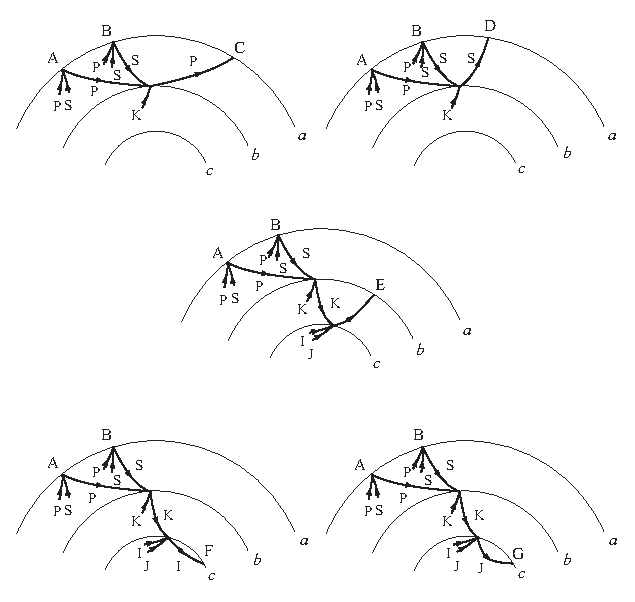
\includegraphics{../figures/chap12/fig14.eps}
\end{center}
\caption[FeynmanRegimeIX]{\label{12.fig.zhao11}
用于区段IX中P-SV波相长干涉分析的“历程”或“费曼”图。
从每一幅图可以分别得到一个在C、D、E、F和G点的相对振幅 
$a_{\rm P}$, $a_{\rm S}$,
$a_{\rm K}$, $a_{\rm I}$ and $a_{\rm J}$ 所满足的线性方程。}
\end{figure}
(\ref{12.limco})--(\ref{12.limco2})这两个条件意味着垂直入射的PKIKP波可以几乎畅通无阻地穿过整个地球,而ScS波和J波则分别在核幔边界和内核边界发生全反射。利用这些$p\approx 0$的结果,
再用三角函数等式合并同类项,我们发现~(\ref{12.UGLY})中令人畏惧的二十个余弦函数项求和可以化简成极为简单的三个函数的乘积:
\eq \label{12.NICE}
(\sin\half\Psi_{\rm ScS})(\cos\half\Psi_{\rm J})
(\sin\half\Psi_{\rm PKIKP})\approx 0,
\en
其中$\Psi_{\rm PKIKP}=\Psi_{\rm PcP}+\Psi_{\rm KiK}+\Psi_{\rm I}
=\omega\tau_{\rm PKIKP}+\pi/2$。我们在第~\ref{sec:8.spherfigs}节中曾经提到区段IX的球型振荡可以经验性地再细分为明显的${\rm ScS}_{\rm SV}$, ${\rm J}_{\rm SV}$和PKIKP家族;(\ref{12.NICE})为这一观察给出了极为清楚的证实与物理解释。这三种类型模式的渐近本征频率分别为
\index{mode!J-equivalent}%
\index{J-equivalent mode}%
\index{mode!ScS-equivalent}%
\index{ScS-equivalent mode}%
\index{mode!PKIKP-equivalent}%
\index{PKIKP-equivalent mode}%
\eq \label{12.ScS}
\omega\tau_{\rm ScS}\approx 2\pi n',
\en
\eq \label{12.Jfreq}
\omega\tau_{\rm J}\approx 2\pi(n''-\fourth),
\en
\eq \label{12.PKIKP}
\omega\tau_{\rm PKIKP}\approx 2\pi(n'''-\fourth),
\en
其中$n'$,$n''$和$n'''$为正整数。径向阶序数$n$可以在对从区段II到区段VIII中的模式计数之后,再把这三个带撇号的量子数按频率排序以后确定。

(\ref{12.ScS})--(\ref{12.Jfreq})与表~\ref{table:SH}中的结果的比较证实${\rm ScS}_{\rm SV}$和${\rm ScS}_{\rm SH}$模式具有相同的渐近本征频率,而${\rm J}_{\rm SV}$和${\rm J}_{\rm SH}$模式的渐近本征频率却是相互交错的,如图~\ref{fig:incoremodes}所示。在此处的分析中,这种不同类型的内核模式之间的交错是由于${\rm J}_{\rm SV}$和${\rm J}_{\rm SH}$的反射系数之间的差别。如果我们换成用位移的纵向分量来进行相长干涉分析,在$p\rightarrow 0$的极限下,这两个内核边界反射系数将会是相等的,这时两种模式之间的交错则是由于${\rm J}_{\rm SV}$在折返时的符号反向。在当前的区段,以${\rm J}_{\rm SV}$为主的模式是在区段VI和VII中出现的那组纯${\rm J}_{\rm SV}$模式的光滑的延伸。后者的渐近本征频率公式为$\omega\tau_{\rm J}=2\pi(n''+\fourth)-\psi_{\rm J}$,其中$\psi_{\rm J}$来自过临界的${\rm J}_{\rm SV}$波的全反射系数$\acute{J}\hspace{-0.4 mm}\grave{J}=\exp(-i\psi_{\rm J})$。

由射线参数$p=0$的P, K和I波的相长干涉而形成的径向模式具有纯压缩型的特征,没有纯粹径向的${\rm ScS}_{\rm SV}$或${\rm J}_{\rm SV}$模式。因为地球的球心$r=0$是一个焦散点,此处射线束的宽度从两个方向而不是一个方向减小为零,因此焦散相移为$\pi$而不是$\pi/2$。这一非几何相移被球心处位移径向向上分量的符号反向抵消了,因而沿径向汇聚的波在球心“折返”时净相移为零。于是,径向模式的渐近本征频率公式成为
\eq \label{12.radfreq}
\omega T_{\rm PKIKP}\approx 2\pi(n+1),
\en
其中$T_{\rm PKIKP}$为沿直线路径穿过地球球心的压缩波的单程走时,$n=n'''-1$为传统的径向阶数。径向模式本征频率(\ref{12.radfreq})是PKIKP本征频率~(\ref{12.PKIKP})在$p=0$的延伸;,$\omega\tau_{\rm PKIKP}$在$p\rightarrow 0$的极限时光滑地趋$\omega T_{\rm PKIKP}-\pi/2$,因为根据Jeans关系式~(\ref{12.Jeans}),在对跖点$\Theta=\pi$处,$\omega p\Theta\rightarrow\pi/2$。(\ref{12.radfreq})中的约等号是由于(\ref{12.limco2})中对反射系数做的近似$\grave{P}\hspace{-0.4 mm}\acute{P}
\approx\grave{K}\hspace{-0.4 mm}\acute{K}\approx 0$。通过较为完整的分析,可以得到改进的包含了轻微的核solotone效应的径向模式本征频率方程
\eqa \label{12.radfreq2} \lefteqn{
\sin\half(\Psi_{\rm PcP}+\Psi_{\rm KiK}+\Psi_{\rm I})} \nonumber \\
&&\mbox{}+\grave{P}\hspace{-0.4 mm}\acute{P}
\sin\half(\Psi_{\rm PcP}-\Psi_{\rm KiK}-\Psi_{\rm I}) \nonumber \\
&&\mbox{}+\grave{P}\hspace{-0.4 mm}\acute{P}\,
\grave{K}\hspace{-0.4 mm}\acute{K}
\sin\half(\Psi_{\rm PcP}-\Psi_{\rm KiK}+\Psi_{\rm I}) \nonumber \\
&&\mbox{}+\grave{K}\hspace{-0.4 mm}\acute{K}
\sin\half(\Psi_{\rm PcP}+\Psi_{\rm KiK}-\Psi_{\rm I})=0.
\ena
从本质上讲,地球表现出“整体地球”的PKIKP模式,而不是近乎独立的PcP, KiK和I模式,因为在核幔边界以及内核边界压缩波的阻抗对比较弱:$\rho_{b+}\alpha_{b+}\approx
\rho_{b-}\alpha_{b-}$和$\rho_{c+}\alpha_{c+}\approx
\rho_{c-}\alpha_{c-}$。

在每一个球型模式射线参数区段里,最终的相长干涉关系都可以写成类似于~(\ref{12.freqIII})和~(\ref{12.UGLY})的形式:
\eq \label{12.geneif}
\sum_{\nu}A_{\nu}\sin\half\Psi_{\nu}=0\qquad
\mbox{or}\qquad\sum_{\nu}A_{\nu}\cos\half\Psi_{\nu}=0.
\en
实数因子$A_{\nu}$是在各个边界上反射-透射系数绝对值与固定$p$的扩散系数比值的乘积组合,而三角函数自变量中的$\Psi_{\nu}$则是有关的振荡型体波相位的线性组合。为计算渐近本征频率,我们将Jeans关系式$\omega=(l+\half)p^{-1}$代入径向量子化关系式~(\ref{12.geneif}),然后在每一个射线参数$p$的区段求解得到的方程。
\begin{sidewaysfigure}
\centering
\rotatebox{270}
{
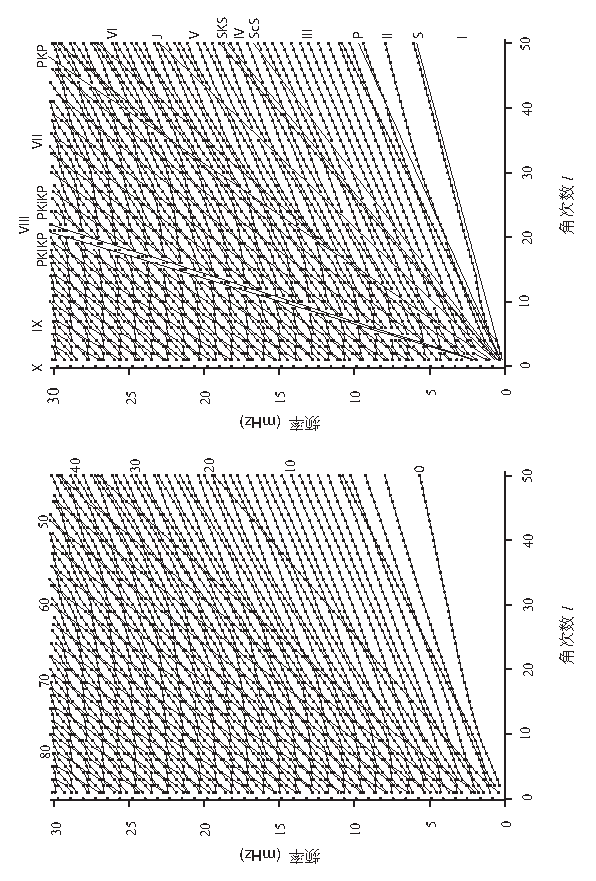
\includegraphics{../figures/chap12/fig15.eps}
}
\caption[Spheroidal Dispersion]{
去掉地壳的1066A模型的球型模式频散曲线图。({\em 左图\/})由数值积分计算的精确本征频率。({\em 右图\/}) P-SV区段II-X的渐近本征频率。左上角部分的放大图见图~\ref{12.fig.blowup}。(由L. Zhao提供)
}
\label{12.fig.zhao19}
\end{sidewaysfigure}
由此对每一个整数次数$l>0$,我们得到一组递减的根$\,{}_0p_l>{}_1p_l>
\cdots>{}_np_l>\cdots$,然后再换算成一组递增的本征频率${}_0\omega_l<{}_1\omega_l<\cdots<{}_n\omega_l<\cdots$。
\begin{figure}[!t]
\begin{center}
\scalebox{1.05}{
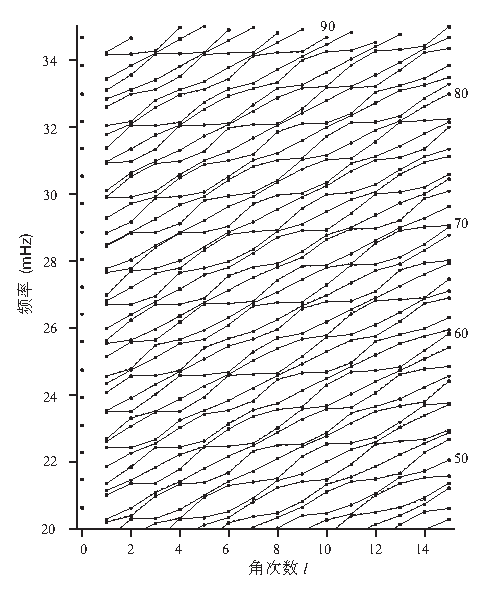
\includegraphics{../figures/chap12/fig16.eps}
}
\end{center}
\caption[BlowupRegimeIX]{\label{12.fig.blowup}
图~\ref{12.fig.zhao19}的球型模式频散曲线图中左上角部分的放大图。由数值积分计算的精确本征频率与用方程~(\ref{12.UGLY})和(\ref{12.radfreq2})计算的区段IX和X的渐近本征频率分别显示为实线连接的实心圆与点线连接的空心圆。整数$n=50$--$90$为径向阶数。(由L. Zhao提供)
是的,确实有空心圆和点线;但是,近乎完美的一致性使我们看不出差别!
}
\end{figure}
\textcolor{red}{核幔边界和内核边界}的Stoneley模式的渐近射线参数分别满足
\eqa \label{12.Stone} \lefteqn{
\rho_{b+}(\beta_{b+}^{-2}-2p^2b^{-2})^2q_{\alpha}(b-)
+\rho_{b-}\beta_{b+}^{-4}q_{\alpha}(b+)} \nonumber \\
&&\mbox{}\qquad\qquad+4\rho_{b+}p^2b^{-2}
q_{\alpha}(b+)q_{\beta}(b+)q_{\alpha}(b-)=0
\ena
和
\eqa \label{12.Stone2} \lefteqn{
\rho_{c-}(\beta_{c-}^{-2}-2p^2c^{-2})^2q_{\alpha}(c+)
+\rho_{c+}\beta_{c-}^{-4}q_{\alpha}(c-)} \nonumber \\
&&\mbox{}\qquad\qquad+4\rho_{c-}p^2c^{-2}
q_{\alpha}(c-)q_{\beta}(c-)q_{\alpha}(c+)=0,
\ena
它们必须插入到本征频率序列的适当位置以保证与传统一致的径向阶数序数。~(\ref{12.Stone})--(\ref{12.Stone2})左边的表达式是在两个边界的反射与透射系数的共同分母。由于$p=0$时~(\ref{12.radfreq2})是$\omega$的单变量方程,因此径向模式的本征频率${}_0\omega_0<{}_1\omega_0<\cdots<{}_n\omega_0<\cdots$可以直接解方程得到。

图~\ref{12.fig.zhao19}展示了在去掉地壳的1066A模型中渐近与精确的频散曲线之间非常好的一致性。标有S, P, ScS, SKS, J, PKI, PKiKP和PKIKP的粗斜线是分隔表12.2中的各个渐近区段的常数射线参数。与环型模式的情形一样,主要的误差出现在这些边界值附近,由于在边界值两边焦散及其它相移的差别使渐近本征频率表现出不连续性。在精确的频散曲线中,由于近掠射和近临界波的隧道效应以及其它相关的有限频率现象会将这些不连续性平滑掉。如图12.16所示,区段IX中阶梯状的PKIKP, ${\rm ScS}_{\rm SV}$和
${\rm J}_{\rm SV}$模式被~(\ref{12.UGLY})式一览无遗地刻画出来。结果中固定$n$的径向分支$\ldots,\;{}_n\omega_{l-1},\; {}_n\omega_l,
\;{}_n\omega_{l+1},\dots$的“交叉回避”是一系列经典与量子力学系统中弱耦合频谱的典型特征(Arnold \citeyear{arnold78})。
\index{mode-ray duality!spheroidal modes|)}%
\index{constructive-interference principle|)}%

\section{正规渐近分析}
\label{12.sec.JWKBS}

上一节所讨论的相长干涉分析为具有两个内部不连续面的地球模型中高频的环型与球型模式和传播的SH与P-SV体波之间的二象性提供了清晰的物理图像。下面我们通过更严格的数学处理来证实前面的结果,并且同时得到相应的径向本征函数的渐近表达式。这一过程的目标是在固定SH或P-SV波的射线参数$p$的情形下,寻求满足的常微分方程和边界条件在高频$\om\rightarrow\infty$时的解。这一分析的基本假设是地球的特性参数$\alpha$、$\beta$、
$\rho$都是平滑变化的,只有在内核边界$r=c$处,核幔边界$r=b$处及自由表面$r=a$处有跃变。我们遵循\textcite{woodhouse78}所阐述的普遍的处理方法,但是我们不是直接进行渐近本征函数的推导,而是寻求将方程组变换到一个更简单的在渐近意义上等价的系统。为便于相高频极限推广,我们首先系统性地把方程改写成$\omega^{-1}$的幂次项形式。对于正的角次数$l>0$,我们究竟是用Jeans关系式$\omega p=l+\half$,还是用下式
\eq \label{12.newp}
\omega p=k=\sqrt{l(l+1)},
\en
来定义射线参数都是无关紧要的,因为这两个定义在$\omega\rightarrow\infty$的极限时是等价的。我们在下面的讨论中采用~(\ref{12.newp})这一稍微方便一些的平方根定义。函数符号上面的一点任然用来表示对半径求导。

\subsection{环型模式}
\index{mode-ray duality!toroidal modes|(}%
\label{12.sec.torasy}

环型模式所满足的一阶线性方程组~(\ref{eq:8.tor1})--(\ref{eq:8.tor2})可以写为矩阵形式
\eq
\dot{\ssf}=\om(\ssA_0+\om^{-1}\ssA_1+\om^{-2}\ssA_2)\ssf.
\label{eq:12.ftor}
\en
(\ref{eq:12.ftor})中未知的位移-牵引力组成的两分量矢量$\ssf$的定义为
\eq \label{12.ftor2}
\ssf=\left(\begin{array}{c} W \\ \om^{-1}T \end{array}\right),
\en
而$2\times 2$矩阵$\ssA_0$、$\ssA_1$和$\ssA_2$为
\begin{displaymath}
\ssA_0=\left(\begin{array}{cc}
0 & \mu^{-1} \\
-\rho+p^2r^{-2}\mu & 0
\end{array}\right),
\end{displaymath}\begin{displaymath}
\ssA_1=\left(\begin{array}{cc}
r^{-1} & 0 \\
0 & -3r^{-1}
\end{array}\right),
\end{displaymath}
\eq
\ssA_2=\left(\begin{array}{cc}
0 & 0 \\
-2r^{-2}\mu & 0
\end{array}\right).
\en
定义~(\ref{12.ftor2})中所隐含的量级关系确保在$\omega\rightarrow\infty$时$\ssf$的两个分量数量级相同。

按照\textcite{richards74}中的渐近势函数表示,我们期望高频本征函数应该与{\em SH 波函数\/}$H$满足相同的径向薛定谔方程
\index{wavefunction!SH}%
\index{Schr\"{o}dinger equation}%
\eq
\ddot{H}+\om^2q_{\beta}^2H=0,
\label{eq:12.helm}
\en
其中$q_{\beta}^2=\beta^{-2}-p^2r^{-2}$。通过定义
\eq
\ssg=\left(\begin{array}{c} H \\
\om^{-1}\dot{H} \end{array}\right),\qquad
\ssQ=\left(\begin{array}{cc}
0 & 1 \\
-q_{\beta}^2 & 0
\end{array}\right),
\en
我们可以将~(\ref{eq:12.helm})写为类似于~(\ref{eq:12.ftor})的矩阵形式:
\eq
\dot{\ssg}=\om\ssQ\ssg.
\label{eq:12.foG}
\en
对于方程~(\ref{eq:12.ftor}),我们寻找如下形式的解$\ssf$
\eq
\ssf=[\,\ssY^{(0)}+\om^{-1}\ssY^{(1)}+\cdots\,]\ssg,
\label{eq:12.bef}
\en
其中矩阵$\ssY^{(0)},\,\ssY^{(1)},\ldots$为待定。将展开式~(\ref{eq:12.bef})代入,并令$\om^{-1}$同幂次项相等,我们可以得到一系列方程,其中前两个为
\eq \label{12.rec1}
\ssA_0\ssY^{(0)}-\ssY^{(0)}\ssQ=\sszero,
\en
\eq \label{12.rec2}
\ssA_0\ssY^{(1)}-\ssY^{(1)}\ssQ=
\dot{\ssY}^{(0)}-\ssA_1\ssY^{(0)}.
\en
假如像前面那样用$p=(l+\half)/\omega$而不是$p=k/\omega$来定义射线参数,只有矩阵$\ssA_2$会改变,而它在零阶和一阶关系~(\ref{12.rec1})--(\ref{12.rec2})中并不出现。

值得注意的是矩阵$\ssQ$和$\ssA_0$可以用一个相似变换联系起来:
\eq
\ssQ=\ssR^{-1}\ssA_0\ssR,
\en
其中
\eq
\ssR=\left(\begin{array}{cc}
\mu^{-1/2} & 0 \\ 0 & \mu^{1/2}
\end{array}\right),\qquad
\ssR^{-1}=\left(\begin{array}{cc}
\mu^{1/2} & 0 \\ 0 & \mu^{-1/2}
\end{array}\right).
\en
这使我们可以方便地将矩阵$\ssY^{(0)},\,\ssY^{(1)},\ldots$用如下变换来表示:
\eq \label{12.YRT}
\ssY^{(0)}=\ssR\ssGamma^{(0)},\qquad
\ssY^{(1)}=\ssR\ssGamma^{(1)},\qquad\cdots,
\en
同时将矩阵$\ssGamma^{(0)},\;\ssGamma^{(1)},\ldots$当做新的未知量。将表达式~(\ref{12.YRT})代入~(\ref{12.rec1})--(\ref{12.rec2}),我们看到$\ssGamma^{(0)},\,\ssGamma^{(1)},\ldots$必须满足
\eq \label{12.rec3}
[\ssQ,\ssGamma^{(0)}]=\sszero,
\en
\eq \label{12.rec4}
[\ssQ,\ssGamma^{(1)}]=\dot{\ssGamma}^{(0)}+(\ssR^{-1}\dot{\ssR}
-\ssR^{-1}\ssA_1\ssR)\ssGamma^{(0)},
\en
其中符号$[\,\cdot\,,\,\cdot\,]$表述括号中矩阵的对易式。(\ref{12.rec3})式表明最低阶未知矩阵乘子$\ssGamma^{(0)}$必须与薛定谔矩阵$\ssQ$是可对易的。很容易证明$\ssQ$与$2\times 2$单位矩阵$\ssI$构成一个完备的对易矩阵集。因此我们可以将$\ssGamma^{(0)}$写为如下形式
\eq
\ssGamma^{(0)}=\gamma_1\ssI+\gamma_2\ssQ,
\label{12.T0is}
\en
其中半径的标量函数$\gamma_1$和
$\gamma_2$仍为待定。

要求得这些函数我们需要考虑一阶关系式~(\ref{12.rec4})。该非齐次方程有特解$\ssGamma^{(1)}$存在的必要且充分的条件是它的右边必须与左边对易算子的零空间正交:
\eq \label{12.cond1}
\mbox{tr}\,[\dot{\ssGamma}^{(0)}+(\ssR^{-1}\dot{\ssR}
-\ssR^{-1}\ssA_1\ssR)\ssGamma^{(0)}]=0,
\en
\eq \label{12.cond2}
\mbox{tr}\,[\ssQ\dot{\ssGamma}^{(0)}+\ssQ(\ssR^{-1}\dot{\ssR}
-\ssR^{-1}\ssA_1\ssR)\ssGamma^{(0)}]=0.
\en
这些存在条件可以化简为未知标量函数的一对一阶微分方程:
\eq \label{12.gam12eqns}
\dot{\gamma}_1+r^{-1}\gamma_1=0,\qquad
\dot{\gamma}_2+(q_{\beta}^{-1}\dot{q}_{\beta}+r^{-1})\gamma_2=0.
\en
方程~(\ref{12.gam12eqns})的解具有如下形式
\eq
\gamma_1=ar^{-1},\qquad
\gamma_2=br^{-1}q_{\beta}^{-1},
\en
其中$a$和$b$b为任意常数。

综合这些结果,我们看出方程~(\ref{eq:12.ftor})的零阶渐近解可以写为
\eq \label{12.frelg}
\ssf=r^{-1}\ssR(a\ssI+bq_{\beta}^{-1}\ssQ)\ssg.
\en
如果我们将薛定谔两分量矢量$\ssg$看作是完全给定的,那么表达式~(\ref{12.frelg})中的常数$a$和$b$就为满足环型模式的边界条件提供了两个自由度。另外一种做法是,我们给定$a$和$b$,将自由度归入薛定谔方程~(\ref{eq:12.foG})的两个线性独立解中。我们采纳后一种方法,为简单起见设定$a=1$和$b=0$,方程~(\ref{12.frelg})于是简化为
\eq \label{12.frelg2}
\ssf=r^{-1}\ssR\ssg,
\en
或是等价的
\eq \label{12.WrelH}
W=\mu^{-1/2}r^{-1}H,
\qquad T=\mu^{1/2}r^{-1}\dot{H}.
\en
如图\textcite{woodhouse78}所展示的,对表达式~(\ref{12.WrelH})更高阶的修正可以用类似方式获得。如前述做法,在$\omega^{-1}$的每一幂次,要想完全确定渐近解,都必须考虑下一幂次的可解性。一阶修正会依赖于剪切波速度和密度的一阶导数$\dot{\beta}$和
$\dot{\rho}$,二阶修正依赖于二阶导数$\ddot{\beta}$和 $\ddot{\rho}$ ,以此类推。零阶表达式~(\ref{12.WrelH})适用于特性参数足够光滑的任何地球模型,其光滑程度由这些导数的大小确定。

总之,我们已经把高频环型模式的位移$W$和相应的牵引力$T$用满足薛定谔方程~(\ref{eq:12.helm})的SH波函数$H$表示。我们将把这些结果用于没有莫霍面以及上地幔不连续面的地球模型,函数$H$在地球球心$r=0$处必须是规则的,而且在内核边界$r=c$,核幔边界$r=b$和自由表面$r=a$处必须满足边界条件$\dot{H}=0$。如果要将这一分析推广到更普遍的模型,只需要牵引力$\mu^{1/2}r^{-1}\dot{H}$在跨越固-固边界$r=d_{\rm SS}$时连续即可。如果模型有一层海水,那么上表面的边界条件则必须施加在海底$r=s$而不是在$r=a$处。原则上,我们可以通过以这些边界条件与连续性条件为约束对薛定谔方程做数值积分来求得环型模式的零阶本征值与本征函数。但是,这种做法有悖常理,因为求解薛定谔方程所需要的计算工作与一点也不比求解精确方程~(\ref{eq:8.tor1})--(\ref{eq:8.btor2})来的要少。本节中所介绍的渐近理论的优势是,它使我们能够用薛定谔方程在$\omega\rightarrow\infty$的极限时的JWKB解来得到$W$
和$T$的{\em 解析表达式\/}。我们在第~\ref{12.sec.jwkb}节先对经典的一维JWKB方法做一个简单的概述,然后在第~\ref{12.sec.asytor}节将其用于环型模式。
\index{mode-ray duality!toroidal modes|)}%

\subsection{球型模式}
\index{mode-ray duality!spheroidal modes|(}%

在$\omega\rightarrow\infty$的极限,自重力对球型简正模式的影响可以放心地忽略。一个无重力的地球中固态区域所满足的$4\times 4$的耦合一阶常微分方程组~(\ref{eq:8.igU})--(\ref{eq:8.igS})可以写成与~(\ref{eq:12.ftor})类似的矩阵形式:
\eq
\dot{\ssf}=\om(\ssA_0+\om^{-1}\ssA_1+\om^{-2}\ssA_2)\ssf.
\label{12.fsph}
\en
此时量级适宜的位移和牵引力4分量矢量为
\pagebreak
\eq
\ssf=\left(\begin{array}{c}
U \\ V \\ \om^{-1}R \\ \om^{-1}S \end{array}\right),
\en
矩阵$\ssA_0$、$\ssA_1$和$\ssA_2$为
\begin{displaymath} \label{12.AS}
\ssA_0=\left(\begin{array}{cccc}
0 & pr^{-1}\lambda\sigma^{-1} & \sigma^{-1} & 0 \\
-pr^{-1} & 0 & 0& \mu^{-1} \\
-\rho & 0 & 0 & pr^{-1} \\
0 & -\rho+4p^2r^{-2}\mu\eta\sigma^{-1} & -pr^{-1}\lambda\sigma^{-1} & 0
\end{array}\right),
\end{displaymath}
\begin{displaymath}
\ssA_1=\left(\begin{array}{cccc}
-2r^{-1}\lambda\sigma^{-1} & 0 & 0 & 0 \\
0 & r^{-1} & 0 & 0 \\
0 & -6pr^{-2}\kappa\mu\sigma^{-1} & -4r^{-1}\mu\sigma^{-1} & 0 \\
-6pr^{-2}\kappa\mu\sigma^{-1} & 0 & 0 & -3r^{-1}
\end{array}\right),
\end{displaymath}
\eq
\ssA_2=\left(\begin{array}{cccc}
0 & 0 & 0 & 0 \\
0 & 0 & 0 & 0 \\
12r^{-2}\kappa\mu\sigma^{-1} & 0 & 0 & 0 \\
0 & -2r^{-2}\mu & 0 & 0
\end{array}\right),
\en
其中$\lambda=\kappa-\twothirds\mu$、
$\sigma=\kappa+\fourthirds\mu$和
$\eta=\kappa+\third\mu$.

我们希望能够把本征函数$U$、$V$、$R$和 $S$用{\em 一对\/}薛定谔方程的解来表示。
\index{Schr\"{o}dinger equation}%
将P波和SV波的波函数分别用$P$和$B$表示,我们指定
\index{wavefunction!SV}%
\index{wavefunction!P}%
\eq
\ddot{P}+\om^2q_{\alpha}^2P=0,\qquad
\ddot{B}+\om^2q_{\beta}^2B=0,
\label{12.helm2}
\en
其中$q_{\alpha}^2=\alpha^{-2}-p^2r^{-2}$和
$q_{\beta}^2=\beta^{-2}-p^2r^{-2}$。
(\ref{12.helm2})中两个方程的独立性意味着P波和SV波的传播在地球结构平滑的区域是相互独立的;在$\omega\rightarrow\infty$时P-SV耦合只发生在内部与外部边界处。要注意,不要把这里的波函数$P$和 $B$与球型模式的完整的$6\times 6$方程组~(\ref{eq:8.foU})--(\ref{eq:8.foK})中用来表示重力增量的相同的符号混淆。通过如下定义
\eq
\ssg=\left(\begin{array}{c}
P \\ \omega^{-1}\dot{P} \\ B \\ \omega^{-1}\dot{B}
\end{array}\right),\qquad
\ssQ=\left(\begin{array}{cccc}
0 & 1 & 0 & 0\\
-q_{\alpha}^2 & 0 & 0 & 0 \\
0 & 0 & 0 & 1 \\
0 & 0 & -q_{\beta}^2 & 0
\end{array}\right),
\en
我们可以把两个独立的薛定谔方程写成与~(\ref{eq:12.foG})相同的形式:
\eq
\dot{\ssg}=\om\ssQ\ssg.
\en
下面我们遵循与SH情形同样的方法,寻求方程~(\ref{12.fsph})的与~(\ref{eq:12.bef})同一形式的渐近解$\ssf$。联系$\ssQ$和$\ssA_0$的变换矩阵$\ssR$和$\ssR^{-1}$为
\begin{displaymath}
\ssR=\rho^{-1/2}\left(\begin{array}{cccc}
0 & 1 & pr^{-1} & 0 \\
pr^{-1} & 0 & 0 & 1 \\
-\rho+2p^2r^{-2}\mu & 0 & 0 & 2pr^{-1}\mu \\
0 & 2pr^{-1}\mu & -\rho+2p^2r^{-2}\mu & 0
\end{array}\right),
\end{displaymath}
\eqa \lefteqn{
\ssR^{-1}=\rho^{-1/2}\left(\begin{array}{cccc}
0 & 2pr^{-1}\mu & -1 & 0 \\
\rho-2p^2r^{-2}\mu & 0 & 0 & pr^{-1} \\
2pr^{-1}\mu & 0 & 0 & -1 \\
0 & \rho-2p^2r^{-2}\mu & pr^{-1} & 0
\end{array}\right).} \\ \nonumber
&&\mbox{}
\ena
$\ssf$和$\ssg$之间最普遍的零阶渐近关系依赖于4个任意常数$a_{\alpha}$、 $b_{\alpha}$、$a_{\beta}$、
$b_{\beta}$,每一个对应于下列一组与$\ssQ$可对易的线性独立矩阵之中的一个:
\begin{displaymath}
\ssI_{\alpha}=\left(\begin{array}{cccc}
1 & 0 & 0 & 0 \\
0 & 1 & 0 & 0 \\
0 & 0 & 0 & 0 \\
0 & 0 & 0 & 0
\end{array}\right),\qquad
\ssQ_{\alpha}=\left(\begin{array}{cccc}
0 & 1 & 0 & 0 \\
-q_{\alpha}^2 & 0 & 0 & 0 \\
0 & 0 & 0 & 0 \\
0 & 0 & 0 & 0
\end{array}\right),
\end{displaymath}
\eq \label{12.fourmat}
\ssI_{\beta}=\left(\begin{array}{cccc}
0 & 0 & 0 & 0 \\
0 & 0 & 0 & 0 \\
0 & 0 & 1 & 0 \\
0 & 0 & 0 & 1
\end{array}\right),\qquad
\ssQ_{\beta}=\left(\begin{array}{cccc}
0 & 0 & 0 & 0 \\
0 & 0 & 0 & 0 \\
0 & 0 & 0 & 1 \\
0 & 0 & -q_{\beta}^2 & 0
\end{array}\right).
\en
取定$a_{\alpha}=a_{\beta}=1$
和$b_{\alpha}=b_{\beta}=0$,我们得到与~(\ref{12.frelg2})类似的表达式:
\eq \label{12.sphasy}
\ssf=r^{-1}\ssR\ssg,
\en
或者等价的
\eq
U=\rho^{-1/2}r^{-1}(\omega^{-1}\dot{P}+pr^{-1}B),
\label{eq:12.Uas}
\en
\eq
V=\rho^{-1/2}r^{-1}(\omega^{-1}\dot{B}+pr^{-1}P),
\label{eq:12.Vas}
\en
\eq
R=-\rho^{1/2}r^{-1}\omega[P-2pr^{-1}\beta^2(\omega^{-1}\dot{B}+pr^{-1}P)],
\label{eq:12.Ras}
\en
\eq
S=-\rho^{1/2}r^{-1}\omega[B-2pr^{-1}\beta^2(\omega^{-1}\dot{P}+pr^{-1}B)].
\label{eq:12.Sas}
\en
P和SV波的薛定谔方程~(\ref{12.helm2})的4个线性独立解提供了满足相应边界条件所需要的自由度。

在液态外核内部牵引力标量$S$消失,切向位移由代数方程$V=-(kr^{-1}R)/(\omega^2\rho)$给定。$2\times2$的常微分方程系统~(\ref{eq:8.igfU})--(\ref{eq:8.igfR})可以写成矩阵形式
\eq \label{12.fsphfl}
\dot{\ssf}=\om(\ssA_0+\om^{-1}\ssA_1)\ssf,
\en
其中
\eq
\ssf=\left(\begin{array}{c} U \\ \om^{-1}R \end{array}\right)
\en
和
\eq
\ssA_0=\left(\begin{array}{cc}
0 & \kappa^{-1}-\rho^{-1}p^2r^{-2} \\
-\rho & 0
\end{array}\right),
\en
\eq
\ssA_1=\left(\begin{array}{cc}
-2r^{-1} & 0 \\
0 & 0
\end{array}\right).
\en
我们希望将$U$和$R$与满足~(\ref{12.helm2})中P波薛定谔方程的波函数$P$联系起来。通过如下定义
\eq
\ssg=\left(\begin{array}{c}
P \\ \omega^{-1}\dot{P}
\end{array}\right),
\qquad\ssQ=\left(\begin{array}{cc}
0 & 1 \\
-q_{\alpha}^2 & 0
\end{array}\right),
\en
我们可以将该方程写为
\eq
\dot{\ssg}=\om\ssQ\ssg.
\en
联系$\ssQ$和$\ssA_0$的矩阵$\ssR$和$\ssR^{-1}$此时成为
\eq
\ssR=\left(\begin{array}{cc}
0 & \rho^{-1/2} \\
-\rho^{1/2} & 0
\end{array}\right),\qquad
\ssR^{-1}=\left(\begin{array}{cc}
0 & -\rho^{1/2} \\
\rho^{-1/2} & 0
\end{array}\right).
\en
为满足薛定谔方程在固-液边界的连续性条件,需要有两个自由度,具有这一性质的$\ssf$和$\ssg$之间恰当的渐近关系为
\eq
\ssf=r^{-1}\ssR\ssg.
\en
相应的液态区域$U$、$V$、$R$、$S$和$P$之间的完整的零阶渐近关系为
\eq \label{12.Uas2}
U=\rho^{-1/2}r^{-1}\om^{-1}\dot{P},
\en
\eq
V=\rho^{-1/2}pr^{-2}P,
\en
\eq
R=-\rho^{1/2}r^{-1}\om P,
\en
\eq \label{12.Sas2}
S=0.
\en
显然,我们也可以通过把~(\ref{eq:12.Uas})--(\ref{eq:12.Sas})中的剪切波速度$\beta$和SV波函数$B$设为零直接得到~(\ref{12.Uas2})--(\ref{12.Sas2})中的结果。

径向模式是纯压缩型的;位移和牵引力标量函数与P波的波函数$P$之间的关系为:$U=\rho^{-1/2}r^{-1}\om^{-1}\dot{P}$、$V=0$、
$R=-\rho^{1/2}r^{-1}\omega P$和 $S=0$。这些结果可以从控制方程组~(\ref{eq:8.Urad})--(\ref{eq:8.Rrad})的渐近分析得到;另外也可以通过在方程组~(\ref{eq:12.Uas})--(\ref{eq:12.Sas})和(\ref{12.Uas2})--(\ref{12.Sas2})中把射线参数$p$和SV波的波函数$B$设为零得到。

总之,我们已经把地球的固态与液态区域的位移和牵引力都用满足薛定谔方程~(\ref{12.helm2})的高频波函数$P$和 $B$表示出来。运动学和动力学边界条件要求在自由表面$r=a$处有
\eq \label{12.sphbc}
P-2pr^{-1}\beta^2(\om^{-1}\dot{B}+pr^{-1}P)=0,
\en
\eq
B-2pr^{-1}\beta^2(\om^{-1}\dot{P}+pr^{-1}B)=0
\label{12.sphbc2}
\en
而在核幔边界$r=b$和内核边界$r=c$处有
\eq \label{12.sphbc3}
B-2pr^{-1}\beta^2(\om^{-1}\dot{P}+pr^{-1}B)=0,
\en
\eq \label{12.sphbc4}
[\rho^{-1/2}(\om^{-1}\dot{P}+pr^{-1}B)]_-^+=0,
\en
\eq \label{12.sphbc5}
[\rho^{1/2}\{P-2pr^{-1}\beta^2(\om^{-1}\dot{B}
+pr^{-1}P)\}]^+_-=0
\en
如果地球有一个海水层,那么~(\ref{12.sphbc3})--(\ref{12.sphbc5})必须也要在海底$r=s$处满足。此外,如果有任何固-固不连续面,则必须在$r=d_{\rm SS}$处有~(\ref{12.sphbc4})--(\ref{12.sphbc5})以及$[\rho^{-1/2}(\om^{-1}\dot{B}+pr^{-1}P)]_-^+=0$。这些条件中$P$和 $B$两个波函数的同时出现反映了P波与SV波在自由表面及各个内部界面处反射与透射时它们之间的相互转换。

更一般地,我们也可以从方程~(\ref{12.fsph})和(\ref{12.fsphfl})的修改过的$4\times 4$和$2\times 2$形式出发进行以上分析,这样虽然忽略了地球的重力势函数的扰动,但是保留了初始重力加速度$g$(见第8.8.6节)。这样做最低阶矩阵$\ssA_0$没有改变,只有$\ssA_1$和$\ssA_2$有变化。这些较高阶矩阵对零阶表达式~(\ref{eq:12.Uas})--(\ref{eq:12.Sas})、
(\ref{12.Uas2})--(\ref{12.Sas2})和(\ref{12.sphbc})--(\ref{12.sphbc5})没有影响。因此,上述结果在{\em Cowling近似\/}下仍然成立。
\index{Cowling approximation}%
在第~\ref{12.sec.sphasy}节中我们将用这些结果来计算地幔球型模式的渐近本征频率和本征函数。
\index{mode-ray duality!spheroidal modes|)}%

\subsection{JWKB近似}
\index{JWKB approximation|(}%
\index{WKBJ|see{JWKB}}%
\index{Schr\"{o}dinger equation|(}%
\label{12.sec.jwkb}

对SH和P-SV波的分析的下一个步骤是用经典JWKB理论寻求径向薛定谔方程的渐近解
\eq
\ddot{X}+\om^2q^2X=0,
\label{12.jwkb}
\en
方程~(\ref{12.jwkb})中半径的未知函数$X$代表~(\ref{eq:12.helm})或(\ref{12.helm2})中三个标量波函数$H$、$P$或 $B$中的任意一个。$q^2=v^{-2}-p^2r^{-2}$是相应的SH, P或SV波的径向慢度的平方,因此乘积$\om q$是局地径向波数。方程~(\ref{12.jwkb})是一个{\em 奇异微扰\/}问题,
\index{perturbation!singular}%
\index{singular perturbation}%
因为导数项与非导数项相比在$\omega\rightarrow\infty$时可以忽略不计。我们仅关注单一折返点$r=R$的情形,在那里$q^2(R)=0$。比较方便的做法是分成三个互相重叠的区段,如图12.17所示:
\begin{enumerate}
\item  $r\ll R$ 且 $q^2<0$;
\item  $r\approx R$ 且 $q^2\approx\gamma(r-R)$,
其中 $\gamma=2v_R^{-3}(R^{-1}v_R-\dot{v}_R)>0$;
\item  $r\gg R$ 且 $q^2>0$.
\end{enumerate}
\begin{figure}[!t]
\centering
\begin{tabular}{lr}
\begin{tabular}{l}
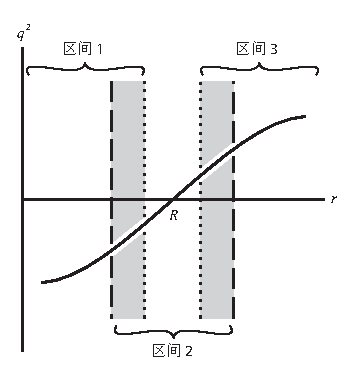
\includegraphics{../figures/chap12/fig17.eps}
\end{tabular}
&
\hspace{0.3cm}
\parbox{3.7cm}{\small
图~12.17. 方程~(\ref{12.jwkb})中平方的径向慢度$q^2(r)$示意图。在其单一零点$r=R$处相应的波折返。在三个区段的每一个区段内分别做JWKB分析,再将得到的解$X_1$、$X_2$和$X_3$在重叠区段(阴影部分)互相做连接。
}
\end{tabular}
\end{figure}
\addtocounter{figure}{1}
遵循~\textcite{bender&orszag78},我们在每一个区段进行独立的渐近分析,然后用{\em 匹配渐近展开方法\/}把得到的结果连起来。
\index{matched asymptotic expansions}%
重要的是三个区段必须按上述列出的顺序考虑,从折返点下方开始,终止于其上方。

在区段1我们寻找JWKB展开形式的解:
\eq \label{12.psiI}
X=[\sA^{(0)}+\omega^{-1}\sA^{(1)}+\cdots]\exp (\omega\Psi),
\en
这里我们希望确定的是振幅$\sA^{(0)},\;\sA^{(1)},\ldots$以及指数上的变量$\Psi$。把我们的猜想解~(\ref{12.psiI})代入薛定谔方程~(\ref{12.jwkb}),并且令$\omega^{-1}$的同幂次项相等,我们得到经典的{\em 程函\/}与{\em 输运方程\/}
\index{eikonal equation}%
\index{transport equation}%
\eq
\dot{\Psi}^2+q^2=0,\qquad\ddot{\Psi}\sA+2\dot{\Psi}\dot{\sA}=0.
\label{12.eikonal}
\en
我们省略了振幅的上角标$\sA^{(0)}=\sA$,因为我们仅关心最低阶的近似。方程~(\ref{12.eikonal})的解为
\eq \label{12.eikonal2}
\Psi=\pm\int_r^R|q|\,dr,\qquad \sA=A|q|^{-1/2},
\en
其中$|q|$是$-q^2$的正平方根,$A$是待定常数。(\ref{12.eikonal2})的前一个等式中的正号对应于远离折返点指数增加,是物理上不允许的。舍弃这一可能性,我们得到区段1的最低阶JWKB解为
\eq \label{12.psiI2}
X_1=A|q|^{-1/2}\exp
\left(-\omega\int_r^R|q|\,dr\right).
\en
公式~(\ref{12.psiI2})代表的是在折返点$r=R$以下指数衰减的{\em 瞬逝波\/}。
\index{evanescent wave}%

在折返点附近,薛定谔方程~(\ref{12.jwkb})简化为{\em 艾里方程\/}
\index{Airy equation}%
\eq \label{12.airy}
\ddot{X}+\omega^2\gamma (r-R)X=0.
\en
方程~(\ref{12.airy})的通解可以用两个线性独立的艾里函数Ai 和 Bi表示成如下形式
\eq
X_2=D\,{\rm Ai}\,[-\omega^{2/3}\gamma^{1/3}(r-R)]
+E\,{\rm Bi}\,[-\omega^{2/3}\gamma^{1/3}(r-R)].
\label{12.yII}
\en
通过匹配~(\ref{12.psiI2})和~(\ref{12.yII})这两个解,常数$D$和 $E$可以可以与瞬逝波振幅$A$联系起来。振幅中因子$|q|^{-1/2}$的发散性使公式~(\ref{12.psiI2})在邻近$r=R$时不适用,同样,公式~(\ref{12.yII})在折返点$r=R$下面过远处也不成立。但是,存在一个重叠区段,在该区段内两个表达式均成立。在此区段,$|q|\approx[\gamma(R-r)]^{1/2}$,我们可以将瞬逝解近似为
\eq
X_1\approx A[\gamma(R-r)]^{-1/4}
\exp[-\twothirds\omega\gamma^{1/2}(R-r)^{3/2}],
\label{12.yIasym}
\en
同时可以利用$x\rightarrow\infty$时的渐进式
\eq
{\rm Ai}(x)\approx\half\pi^{-1/2}x^{-1/4}\exp(-\twothirds x^{3/2}),
\en
\eq
{\rm Bi}(x)\approx\pi^{-1/2}x^{-1/4}\exp(\twothirds x^{3/2})
\en
将折返点的解~(\ref{12.yII})表示成
\eqa
\lefteqn{X_2\approx\pi^{-1/2}
\gamma^{-1/12}\omega^{-1/6}(R-r)^{-1/4}} \nonumber \\
&&\mbox{}\quad\times\left\{\half D\exp[-\twothirds
\omega\gamma^{1/2}(R-r)^{3/2}]\right. \nonumber \\
&&\mbox{}\qquad\qquad\left.+E\exp[\twothirds\omega
\gamma^{1/2}(R-r)^{3/2}]\right\}.
\label{12.yIIasym1}
\ena
通过比较两个重叠区段的解~(\ref{12.yIasym})和~(\ref{12.yIIasym1}),我们看到$D=2\pi^{1/2}\gamma^{-1/6}\omega^{1/6}A$和 $E=0$。于是,在折返点附近$r\approx R$的解成为
\eq
X_2=2\pi^{1/2}A\gamma^{-1/6}\omega^{1/6}
{\rm Ai}\,[-\omega^{2/3}\gamma^{1/3}(r-R)].
\label{12.yII2}
\en
这里的匹配过程确保~(\ref{12.yII2})是区段1中的瞬逝解~(\ref{12.psiI2})在区段2中的光滑延伸。

在$r\gg R$区段,我们同样将猜想解~(\ref{12.psiI})代入薛定谔方程~(\ref{12.jwkb})。因为平方的径向慢度在此区段为正,解不再是瞬逝的,而是振荡型的:
\eqa
\lefteqn{X_3=Fq^{-1/2}\exp\left(i\omega
\int_R^rq\,dr\right)} \nonumber \\
&&\qquad\mbox{}+Gq^{-1/
2}\exp\left(-i\omega\int_R^rq\,dr\right),
\label{12.yIII}
\ena
其中$q$表示$q^2$的正平方根。通过在~(\ref{12.yII2})和~(\ref{12.yIII})这两个解的重叠区段做匹配,可以确定常数$F$和 $G$。在$x\rightarrow-\infty$的极限下,艾里函数~(\ref{12.yII2})的渐近表达式为
\eq
{\rm Ai}(x)\approx\pi^{-1/2}(-x)^{-1/4}\sin[\twothirds(-x)^{3/2}
+\pi/4],
\en
因而
\eq
X_2\approx 2A[\gamma(r-R)]^{-1/4}\sin[\twothirds\omega
\gamma^{1/2}(r-R)^{3/2}+\pi/4].
\label{12.yIIasym2}
\en
另一方面,在重叠区段公式~(\ref{12.yIII})可以写成
\eqa
\lefteqn{X_3\approx F[\gamma(r-R)]^{-1/4}\exp
[\twothirds i\omega\gamma^{1/2}(r-R)^{3/2}]} \nonumber \\
&&\qquad\mbox{}+G[\gamma(r-R)]^{-1/4}\exp
[-\twothirds i\omega\gamma^{1/2}(r-R)^{3/2}].
\label{12.yIIIasym}
\ena
比较~(\ref{12.yIIasym2})和~(\ref{12.yIIIasym}),我们得到$F=-iA\exp(i\pi/4)$和$G=iA\exp(-i\pi/4)$。因此,折返点上面的渐近解为
\eq
X_3=2Aq^{-1/2}\cos\left(\omega\int_R^rq\,dr-\frac{\pi}{4}
\right).
\label{12.yIII2}
\en
(\ref{12.psiI2})和~(\ref{12.yIII2})这两个表达式之间的关系式$A|q|^{-1/2}\exp
(-\omega\int_r^R|q|\,dr)
\Longrightarrow 2Aq^{-1/2}\cos
(\omega\int_R^rq\,dr-\pi/4)$                                             
常常被称为{\em JWKB 连接公式\/},
\index{connection formula}%
\index{JWKB connection formula}%
因为它用折返点下面的瞬逝解来确定折返点上面的振荡解的振幅和相位。表~\ref{table:12.jwkb}总结了所有三个区段的渐近分析的最终结果。

\begin{table}[!b]
\centering
\begin{tabular}{|c|c|l|} \hline
       &          &        \\
区段 & 位置 & \hspace{1.5 cm}渐近解 \\
       &          &        \\ \hline
       &          &        \\
1 & $r\ll R$ & $\displaystyle X_1=A|q|^{-1/2}\exp\left(-\omega
\int_r^R|q|\,dr\right)$ \\
       &          &         \\
2 & $r\approx R$ & $\displaystyle X_2=2\pi^{1/2}A
\gamma^{-1/6}\omega^{1/6}{\rm Ai}\,[-\omega^{2/3}\gamma^{1/3}(r-R)]$ \\
       &          &         \\
3 & $r\gg R$ & $\displaystyle X_3=
2Aq^{-1/2}\cos\left(\omega\int_R^rq\,dr
-\frac{\pi}{4}\right)$ \\
       &          &         \\ \hline
\end{tabular}
\caption[jwkbmatch]{
图12.17中所示的薛定谔方程~(\protect\ref{12.jwkb})的三个区段的渐近解。JWKB波函数$X$在折返点$r=R$下面为瞬逝型,在折返点上面为振荡型。$A$为任意的归一化常数。
}
\label{table:12.jwkb}
\end{table}

值得注意的是,三个解$X_1$,
$X_2$ 和 $X_3$可以合并成为一个单一的{\em 一致有效\/}的近似表达式,称为{\em Langer近似\/}:
\index{Langer approximation}%
\eq
X=2\pi^{1/2}A\,\chi^{1/6}(-q^2)^{-1/4}{\rm Ai}(\chi^{2/3}),
\label{12.langer}
\en
其中$\chi=-\frac{3}{2}\omega\int_R^r\,(-q^2)^{1/2}\,dr$。这一近似的正确性虽然不是一目了然的,但是,通过在所有三个区段上展示该近似与表~\ref{table:12.jwkb}中给出的结果在渐近的意义上是等价的,可以很容易地验证。公式~(\ref{12.langer})仅仅适用于折返半$r=R$远离核幔边界$r=b$这种不连续面去情况。对于更普遍的情况,有必要同时保留${\rm Bi}(\chi^{2/3})$ 和 ${\rm Ai}(\chi^{2/3})$以便考虑近掠射波的隧道效应(Woodhouse \citeyear{woodhouse78})。
\index{JWKB approximation|)}%
\index{Schr\"{o}dinger equation|)}%

\subsection{环型模式回顾}
\index{mode-ray duality!toroidal modes|(}%
\label{12.sec.asytor}

在本节我们用第~\ref{12.sec.torasy}节和第~\ref{12.sec.jwkb}节中的JWKB分析来确定仅有内核边界和核幔边界两个内部不连续面的地球模型中的环型模式的本征频率和本征函数。我们首先考虑与地幔中的SH波等价的区段II中的模式。
\index{SH wave}%
在此区段内平方的径向慢度$q_{\beta}^2=\beta^{-2}-p^2r^{-2}$在折返半径$r=R_{\rm S}$处有单个零点。在折返点之上的振荡型区域$R_{\rm S}\ll r\leq a$,SH波的波函数及其导数可以表示成
\eq
H=2Aq_{\beta}^{-1/2}\cos\left(\omega
\int_{R_{\rm S}}^rq_{\beta}\,dr
-\frac{\pi}{4}\right),
\label{12.Sasym}
\en
\eq
\dot{H}=-2\omega Aq_{\beta}^{1/2}
\sin\left(\omega\int_{R_{\rm S}}^rq_{\beta}\,dr
-\frac{\pi}{4}\right),
\label{12.Sasym2}
\en
这里在求导时我们忽略了$\omega^{-1}$的高阶项。渐近本征频率可以由自由表面边界条件$\dot{H}=0$      确定。取~(\ref{12.Sasym2})在$r=a$处的值,我们得到渐近量子化条件
\eq \label{12.newfreq1}
\omega\tau_{\rm S}=2\pi(n+5/4),
\en
其中$\tau_{\rm S}$为截距时间,$n$为径向阶数。这一结果与我们在第~\ref{12.sec.TOR}节中用更基本而物理上更直观的相长干涉观念得到的结果完全一样。

与~(\ref{12.newfreq1})中的本征频率相应的在$R_{\rm S}\ll r\leq a$区域内的振荡型JWKB本征函数为
\eq \label{12.Wosc}
W=2A\mu^{-1/2}r^{-1}q_{\beta}^{-1/2}\cos
\left(\omega\int_{R_{\rm S}}^rq_{\beta}\,dr
-\frac{\pi}{4}\right).
\en
在折返半径之下,$r\ll R_{\rm S}$,有瞬逝解:
\eq
W=A\mu^{-1/2}r^{-1}|q_{\beta}|^{-1/2}\exp\left(-\omega
\int_r^{R_{\rm S}}|q_{\beta}|\,dr\right).
\en
常数$A$可以从环型模式的归一化关系中得到:
\eq \label{12.Tnorm}
\int_b^a\rho W^2\,r^2dr=1.
\en
\textcite{bender&orszag78}讨论了在有折返点时应如何计算JWKB解的归一化积分。它们证明了,依照Riemann-Lebesque公理,
\index{Riemann-Lebesgue lemma}%
三个区段的总体贡献在渐近的意义上等价于将振荡项$\cos^2(\omega\int_{R_{\rm S}}^a
q_{\beta}\,dr -\pi/4)$用其平均值$1/2$替换之后从$r=R_{\rm S}$积分:
\eq
\int_b^a\rho W^2\,r^2dr=2A^2\int_{R_{\rm S}}^a
\beta^{-2}q_{\beta}^{-1}\,dr.
\en
因此$A=T_{\rm S}^{-1/2}$,其中$T_{\rm S}$是S波走时。

在区段III,SH波的波函数在整个地幔$b\leq r\leq a$都是振荡型的:
\eqa \label{12.ScSasy}
\lefteqn{H=Aq_{\beta}^{-1/2}\exp\left(i\omega
\int_b^rq_{\beta}\,dr\right)} \nonumber \\
&&\qquad\qquad\mbox{}+Bq_{\beta}^{-1/2}\exp
\left(-i\omega\int_b^rq_{\beta}\,dr\right),
\ena
\eqa \label{12.ScSasy2}
\lefteqn{\dot{H}=
i\omega Aq_{\beta}^{1/2}\exp\left(i\omega
\int_b^rq_{\beta}\,dr\right)} \nonumber \\
&&\qquad\qquad\mbox{}-i\omega Bq_{\beta}^{1/2}
\exp\left(-i\omega\int_b^rq_{\beta}\,dr\right),
\ena
其中$A$ 和 $B$为任意常数。
\begin{table}[!b]
\centering
\begin{tabular}{|c|c|l|} \hline
       &           &      \\
区段 & 类型 & \hspace{0.7 cm}归一化位移本征函数 \\
       &           &      \\ \hline
       &           &       \\
I & --- & \hspace{1.6 cm}仅有瞬逝 SH 波 \\
       &           &        \\
II & SH &
$\displaystyle W=2T_{\rm S}^{-1/2}\mu^{-1/2}r^{-1}q_{\beta}^{-1/2}
\cos\left(\omega\int_{R_{\rm S}}^rq_{\beta}\,dr-\frac{\pi}{4}\right)$ \\
       &           &        \\
III & ${\rm ScS}_{\rm SH}$ &
$\displaystyle W=2T_{\rm ScS}^{-1/2}\mu^{-1/2}r^{-1}q_{\beta}^{-1/2}
\cos\left(\omega\int_b^rq_{\beta}\,dr\right)$ \\
       &           &       \\
IV & ${\rm J}_{\rm SH}$ &
$\displaystyle W=2T_{\rm J}^{-1/2}\mu^{-1/2}r^{-1}q_{\beta}^{-1/2}
\cos\left(\omega\int_{R_{\rm J}}^rq_{\beta}\,dr-\frac{\pi}{4}\right)$ \\
       &           &       \\ \hline
\end{tabular}
\caption[toreifs]{
仅有两个内部不连续面的地球模型中SH波的全部四个射线参数区段的渐近归一化本征函数$W$。区段III中的表达式适用于整个地幔$b\leq r\leq a$,而区段II和IV中的表达式仅适用于地幔和内核中折返点之上的振荡型区域$R_{\rm S}\ll r\leq a$ 或 $R_{\rm J}\ll r\leq c$。在折返点之下的区域$r\ll R_{\rm S}$ 和 $r\ll R_{\rm J}$,相应的SH和${\rm J}_{\rm SH}$本征函数为瞬逝型。
}
\label{12.table.toreifs}
\end{table}
在核幔边界$r=b$处的边界条件$\dot{H}=0$意味着$B=A$。相应的自由表面$r=a$处的条件则提供量子化条件
\eq
\omega\tau_{\rm ScS}=2\pi(n+1),
\label{12.newfreq3}
\en
诚如预期的,上式与~(\ref{12.freq3})一样。${\rm ScS}_{\rm SH}$模式的本征函数的JWKB表达式为
\eq
W=2A\mu^{-1/2}r^{-1}q_{\beta}^{-1/2}
\cos\left(\omega\int_b^rq_{\beta}\,dr\right).
\en
Riemann-Lebesque公理仍然可以用来计算归一化积分~(\ref{12.Tnorm}),结果为
$A=T_{\rm ScS}^{-1/2}$.\vspace{-0.5mm}
\begin{figure}[!t]
\begin{center}
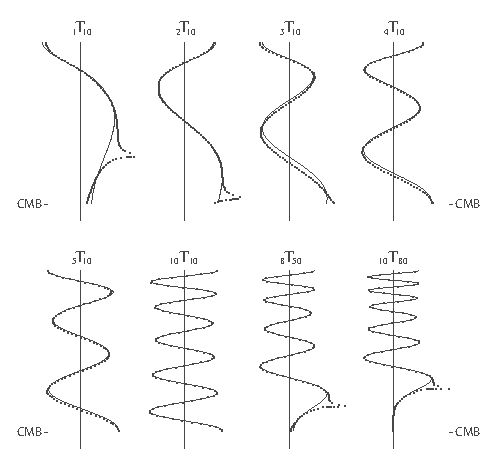
\includegraphics{../figures/chap12/fig18.eps}
\end{center}
\caption[W Comparison]{\label{12.fig.Wplot}
几个环型模式的精确({\em 实线\/})与渐近({\em 点线\/})本征函数$W$。垂直轴为去掉地壳的1066A模型中地表以下的深度,图中标出了核幔边界 (CMB) 的位置。模式${}_1{\rm T}_{10}$、 ${}_2{\rm T}_{10}$、
${}_8{\rm T}_{50}$ 和 ${}_{10}{\rm T}_{80}$为有折返点的SH等价模式,在下地幔的折返点$r=R_{\rm S}$处$W_{\rm JWKB}$发散。模式${}_3{\rm T}_{10}$、${}_4{\rm T}_{10}$、
${}_5{\rm T}_{10}$ 和 ${}_{10}{\rm T}_{10}$为${\rm ScS}_{\rm SH}$等价模式,没有折返点。(由L. Zhao提供)
}
\end{figure}

表12.4中总结了环型模式的所有四个区段里的振荡型JWKB本征函数。区段IV中内核模式的结果与区段II中的完全一样,只需把$\tau_{\rm S}$
和 $T_{\rm S}$分别换成$\tau_{\rm J}$
和 $T_{\rm J}$。这两个区段上本征函数的驻波表达式中的$\pi/4$与折返SH波产生的$\pi/2$焦散相移相一致。图~\ref{12.fig.Wplot}中比较了几个地幔环型模式的精确与渐近的本征函数$W$。两者普遍有很好的一致性甚至包括${}_n{\rm T}_l$中$n\ll l/4$的勒夫波等价模式。主要的差别出现在折返半径$r=R_{\rm S}$附近,那里渐近表达式振幅中的因子$q_{\beta}^{\raise-.8ex\hbox{$\scriptstyle -1/2$}}$ 发散。这一发散是JWKB近似的内在的非一致有效特性。

\textcite{kennett&nolet79}使用第~\ref{12.sec.jwkb}中介绍的Langer近似改进了区段II和III的交界处$p\!=\!b/\beta_{b+}$附近的过渡模式的结果。不连续的本征频率公式$\omega\tau_{\rm S}=2\pi(n+5/4)$
和 $\omega\tau_{\rm ScS}=2\pi(n+1)$被单一的渐近公式$\omega\tau_{\rm S\hspace{0.2 mm}+\hspace{0.2 mm}ScS}=2\pi(n+\delta)$取代,其中的$\delta$在$5/4$与1之间光滑地变化。$2\pi(\delta-1)$就是一个频率为$\omega$的SH\hspace{0.3 mm}+\hspace{0.3 mm}${\rm ScS}_{\rm SH}$波与核幔边界相互作用所产生的相移。在他们的分析中也考虑了过渡带中模型参数的导数$\dot{\beta}$ 和 $\dot{\rho}$和  的一阶效应。
\index{mode-ray duality!toroidal modes|)}%

\subsection{球型模式回顾}
\index{mode-ray duality!spheroidal modes|(}%
\label{12.sec.sphasy}

球型模式的渐近分析也必须以同样方式进行:按射线参数区间一个一个来做。因为本征函数的表达式非常冗长,我们这里仅仅呈现区间III中与折返P和SV波等价的模式的结果。跟前面一样,我们局限于一个没有海水层与内部固-固不连续面的地壳模型。薛定谔方程~(\ref{12.helm2})的振荡型JWKB解可以写成
\eq
P=2Dq_{\alpha}^{-1/2}\sin\left(\omega
\int_{R_{\rm P}}^rq_{\alpha}\,dr
+\frac{\pi}{4}\right),
\label{eq:12.PI}
\en
\eq
\dot{P}=2\omega Dq_{\alpha}^{1/2}\cos\left(\omega
\int_{R_{\rm P}}^rq_{\alpha}\,dr
+\frac{\pi}{4}\right)
\label{eq:12.dotPI}
\en
以及
\eq
B=2Eq_{\beta}^{-1/2}
\cos\left(\omega\int_{R_{\rm S}}^rq_{\beta}\,dr-\frac{\pi}{4}\right),
\label{eq:12.BI}
\en
\eq
\dot{B}=-2\omega Eq_{\beta}^{1/2}
\sin\left(\omega\int_{R_{\rm S}}^rq_{\beta}\,dr-\frac{\pi}{4}\right),
\label{eq:12.dotBI}
\en
其中$D$ 和 $E$为常数,$q_{\alpha}^2=\alpha^{-2}-p^2r^{-2}$,$q_{\beta}^2=\beta^{-2}-p^2r^{-2}$。将表达式~(\ref{eq:12.PI})--(\ref{eq:12.dotBI})代入自由表面动力学边界条件~(\ref{12.sphbc})--(\ref{12.sphbc2}),我们得到联系$D$ 和 $E$这两个常数的方程组:
\eq
\left(\begin{array}{cc}
\zeta_{\alpha}\sin\half\Psi_{\rm P}
& \xi_{\beta}\sin\half\Psi_{\rm S} \\
\vspace{-0.5 mm} & \vspace{-0.5 mm} \\
-\xi_{\alpha}\cos\half\Psi_{\rm P}
& \zeta_{\beta}\cos\half\Psi_{\rm S}
\end{array}\right)
\left(\begin{array}{c} D \\
\vspace{-0.5 mm} \\ E \end{array}\right)
=\left(\begin{array}{c} 0
\vspace{-0.5 mm} \\ \\ 0 \end{array}\right),
\label{eq:12.det}
\en
其中$\Psi_{\rm P}=\omega\tau_{\rm P}+\pi/2$ 和
$\Psi_{\rm S}=\omega\tau_{\rm S}-\pi/2$。
对于P和SV波,$\zeta$ 和 $\xi$的定义均为
\eq
\zeta=(\beta_a^{-2}-2p^2a^{-2})q^{-1/2}(a),\qquad
\xi=2pa^{-1}q^{1/2}(a).
\en
方程~(\ref{eq:12.det})有解的条件是与$D$ 和 $E$相乘的矩阵的行列式为零,该有解条件可以化为
\eq \label{12.spheif}
\sin\half(\Psi_{\rm S}+\Psi_{\rm P})
+\left[\frac{\xi_{\alpha}\xi_{\beta}-\zeta_{\alpha}\zeta_{\beta}}
{\xi_{\alpha}\xi_{\beta}+\zeta_{\alpha}\zeta_{\beta}}\right]
\sin\half(\Psi_{\rm S}-\Psi_{\rm P})=0.
\en
方程~(\ref{12.spheif})与区间III中的渐近本征频率关系~(\ref{12.freqIII})是等价的。很容易可以证明方括号中的表达式就是自由表面的SV波反射系数$\acute{S}\hspace{-0.4 mm}\grave{S}$。值得注意的是~(\ref{12.coef4})中的系数是一个{\em 平面\/}波在{\em 平面\/}表面的反射系数,却自然地出现在当前的分析中。从本质上说,这当然是高频波与边界作用的局地平面特性的结果。

一旦从方程~(\ref{12.spheif})中计算出本征频率,对常数$D$和 $E$的约束可以通过求解~(\ref{eq:12.det})中的任何一个方程得到。我们得到$D=A\hspace{0.2 mm}\zeta_{\beta}\cos\half\Psi_{\rm S}$和
$E=A\hspace{0.2 mm}\xi_{\alpha}\cos\half\Psi_{\rm P}$,其中$A$为待定的归一化常数。利用表达式~(\ref{eq:12.Uas})和~(\ref{eq:12.Vas}),我们得到球型模式的本征函数:
\eqa \label{12.UIII}
\lefteqn{U=2A\rho^{-1/2}r^{-1}\biggl[(\zeta_{\beta}\cos\half\Psi_{\rm S})
q_{\alpha}^{1/2}\cos\left(\omega\int_{R_{\rm P}}^rq_{\alpha}\,dr
+\frac{\pi}{4}\right)} \nonumber \\
&&\mbox{}+(\xi_{\alpha}\cos\half\Psi_{\rm P})
p\hspace{0.2 mm}r^{-1}q_{\beta}^{-1/2}
\cos\left(\omega\int_{R_{\rm S}}^rq_{\beta}\,dr
-\frac{\pi}{4}\right)\biggr],
\ena
\eqa \label{12.VIII}
\lefteqn{V=2A\rho^{-1/2}r^{-1}\biggl[(\zeta_{\beta}\cos\half\Psi_{\rm S})
p\hspace{0.2 mm}r^{-1}q_{\alpha}^{-1/2}
\sin\left(\omega\int_{R_{\rm P}}^rq_{\alpha}\,dr
+\frac{\pi}{4}\right)} \nonumber \\
&&\quad\mbox{}-(\xi_{\alpha}\cos\half\Psi_{\rm P})q_{\beta}^{1/2}
\sin\left(\omega\int_{R_{\rm S}}^rq_{\beta}\,dr
-\frac{\pi}{4}\right)\biggr].
\ena
常数$A$可以用球型模式的归一化关系确定:
\eq \label{12.normal}
\int_0^a\rho(U^2+V^2)\,r^2dr=1.
\en
从两个折返半径$r=R_{\rm P}$和$r=R_{\rm S}$开始积分,使用Riemann-Lebesgue公理,我们得到
\eq
A=[(\zeta_{\beta}\cos\half\Psi_{\rm S})^2T_{\rm P}
+(\xi_{\alpha}\cos\half\Psi_{\rm P})^2T_{\rm S}]^{-1/2},
\en
其中$T_{\rm P}$和$T_{\rm S}$分别为P波和SV波的走时。
\index{travel time!P-wave}%
\index{travel time!SV-wave}%

我们可以把归一化关系~(\ref{12.normal})改写成
\eq \label{12.normal2}
f_{\rm P}+f_{\rm S}=1,
\en
其中
\eq \label{12.fdef1}
f_{\rm P}=\frac{(\zeta_{\beta}\cos\half\Psi_{\rm S})^2T_{\rm P}}
{(\zeta_{\beta}\cos\half\Psi_{\rm S})^2T_{\rm P}+
(\xi_{\alpha}\cos\half\Psi_{\rm P})^2T_{\rm S}},
\en
\eq \label{12.fdef2}
f_{\rm S}=\frac{(\xi_{\alpha}\cos\half\Psi_{\rm P})^2T_{\rm S}}
{(\zeta_{\beta}\cos\half\Psi_{\rm S})^2T_{\rm P}+
(\xi_{\alpha}\cos\half\Psi_{\rm P})^2T_{\rm S}}.
\en
$f_{\rm P}$ 和 $f_{\rm S}$ 这两个量是模式中分别以{\em P 波\/}波和{\em SV 波\/}波形式的{\em 动能占比\/}。
\index{P wave}%
\index{SV wave}%
在模式-射线二象性的讨论中,这些能量都只能在渐近的意义上定义。归一化的振荡型本征函数可以用$f_{\rm P}$ 和 $f_{\rm S}$表示成如下形式
\index{fractional energy}%
\index{energy!fractional}%
\eqa \label{12.UIIIn}
\lefteqn{U=2\rho^{-1/2}r^{-1}\biggl[f_{\rm P}^{1/2}T_{\rm P}^{-1/2}
q_{\alpha}^{1/2}\cos\left(\omega\int_{R_{\rm P}}^rq_{\alpha}\,dr
+\frac{\pi}{4}\right)} \nonumber \\
&&\mbox{}+f_{\rm S}^{1/2}T_{\rm S}^{-1/2}
p\hspace{0.2 mm}r^{-1}q_{\beta}^{-1/2}
\cos\left(\omega\int_{R_{\rm S}}^rq_{\beta}\,dr
-\frac{\pi}{4}\right)\biggr],
\ena
\eqa \label{12.VIIIn}
\lefteqn{V=2\rho^{-1/2}r^{-1}\biggl[f_{\rm P}^{1/2}T_{\rm P}^{-1/2}
p\hspace{0.2 mm}r^{-1}q_{\alpha}^{-1/2}
\sin\left(\omega\int_{R_{\rm P}}^rq_{\alpha}\,dr
+\frac{\pi}{4}\right)} \nonumber \\
&&\quad\mbox{}-f_{\rm S}^{1/2}T_{\rm S}^{-1/2}q_{\beta}^{1/2}
\sin\left(\omega\int_{R_{\rm S}}^rq_{\beta}\,dr
-\frac{\pi}{4}\right)\biggr].
\ena
值得注意的是位移的径向分量$U$在$r=R_{\rm S}$处发散,但却在$r=R_{\rm P}$处为零。相反,切向或水平向位移$V$则在$r=R_{\rm P}$处发散,而在$r=R_{\rm S}$处为零。
\index{particle motion!body-wave}%
\index{polarization!body-wave}%
\index{body-wave polarization}%
这一行为很容易通过考虑相应的射线来理解:伴随P波的质点运动在$r=R_{\rm P}$完全在纵向上,而伴随SV波的却是纯径向的。JWKB渐近表达式~(\ref{12.UIIIn})--(\ref{12.VIIIn})中的P波和SV波两项分别在各自的振荡型区域$R_{\rm P}\ll r\leq a$和 $R_{\rm S}\ll r\leq a$中成立。

其它几个球型模式射线参数区间的渐近本征函数$U$,$V$可以用类似的做法得到。普遍来说,除了自由表面的边界条件~(\ref{12.sphbc})--(\ref{12.sphbc2})之外,还必须使用核幔边界$r=b$和内核边界$r=c$处的边界条件~(\ref{12.sphbc3})--(\ref{12.sphbc5})。\textcite{zhao&dahlen95a}给出了有两个内部固-液不连续面的地壳模型的一套完整的结果,包括在定量上有意义的瞬逝波部分。
\begin{table}[!t]
\centering
\begin{tabular}{|c|l|} \hline
                  &      \\
模式类型 & \hspace{0.9 cm}归一化位移本征函数  \\
                  &      \\ \hline
                  &      \\
& $\displaystyle U\approx 2T_{\rm ScS}^{-1/2}\rho^{-1/2}p\hspace{0.2 mm}r^{-2}
q_{\beta}^{-1/2}\sin\left(\omega\int_b^rq_{\beta}\,dr\right)$ \\
${\rm ScS}_{\rm SV}$  &        \\
& $\displaystyle V\approx 2T_{\rm ScS}^{-1/2}\rho^{-1/2}r^{-1}
q_{\beta}^{1/2}\cos\left(\omega\int_b^rq_{\beta}\,dr\right)$ \\
       &         \\ \hline
                  &      \\
& $\displaystyle U\approx -2T_{\rm J}^{-1/2}\rho^{-1/2}p\hspace{0.2 mm}r^{-2}
q_{\beta}^{-1/2}\cos\left(\omega\int_{R_{\rm J}}^rq_{\beta}\,dr
-\frac{\pi}{4}\right)$ \\
${\rm J}_{\rm SV}$  &        \\
& $\displaystyle V\approx 2T_{\rm J}^{-1/2}\rho^{-1/2}r^{-1}
q_{\beta}^{1/2}\sin\left(\omega\int_{R_{\rm J}}^rq_{\beta}\,dr
-\frac{\pi}{4}\right)$ \\
       &         \\ \hline
                  &      \\
& $\displaystyle U\approx 2T_{\rm PKIKP}^{-1/2}\rho^{-1/2}r^{-1}
q_{\alpha}^{1/2}\cos\left(\omega\int_{R_{\rm I}}^rq_{\alpha}\,dr
+\frac{\pi}{4}\right)$ \\
PKIKP  &        \\
& $\displaystyle V\approx 2T_{\rm PKIKP}^{-1/2}\rho^{-1/2}p\hspace{0.2 mm}r^{-2}
q_{\alpha}^{-1/2}\sin\left(\omega\int_{R_{\rm I}}^rq_{\alpha}\,dr
+\frac{\pi}{4}\right)$ \\
       &         \\ \hline
                  &      \\
& $\displaystyle U\approx 2T_{\rm PKIKP}^{-1}\rho^{-1/2}r^{-1}\alpha^{-1/2}
\cos\left(\omega\int_0^r\alpha^{-1}\,dr\right)$ \\
径向模式 &         \\
& $V=0$ \\
       &         \\ \hline
\end{tabular}
\caption[sphereifs]
{
区间IX和X中模式的渐近归一化本征函数。${\rm ScS}_{\rm SV}$表达式适用于整个地幔$b\leq r\leq a$,而在其下的液态外核$c\leq r\leq b$则有相应的瞬逝波形式。${\rm J}_{\rm SV}$表达式在内核的振荡型区域$R_{\rm J}\ll r\leq c$成立,而在内核折返点之下$0\leq r\ll R_{\rm J}$的区域以及液态外核$c\leq r\leq b$则有瞬逝波形式。PKIKP表达式在其振荡型区域$R_{\rm I}\ll r\leq a$成立。径向模式的表达式适用于所有$0\ll r\leq a$的区域。
}
\label{12.table.UV}
\end{table}
在区间IX和X,我们必须考虑地幔中的上行与下行的P波和SV波,在液态外核中的上行与下行的K波,和固态内核中的折返以及瞬逝的I和${\rm J}_{\rm SV}$波。得到的$U$和$V$的JWKB表达式非常复杂,但是在近垂直入射角近似下
$\grave{P}\hspace{-0.4 mm}\acute{P}\approx
\grave{K}\hspace{-0.4 mm}\acute{K}\approx 0$,它们可以化简为一组分解的${\rm ScS}_{\rm SV}$、${\rm J}_{\rm SV}$和PKIKP模式的简洁的结果。我们在表12.5中列出了区间IX和X中简化的本征函数表达式。如同预期的,径向模式就是PKIKP模式在$p\rightarrow 0$时的极限结果。值得注意的是,${\rm J}_{\rm SV}$ 和
${\rm J}_{\rm SH}$内核模式的切向位移分别形如$V\hspace{-0.6 mm}\sim\hspace{-0.3 mm}
\sin(\om\int_{R_{\rm J}}^rq_{\beta}\,dr-\pi/4)$ 和
$W\hspace{-0.6 mm}\sim\hspace{-0.3 mm}
\cos(\om\int_{R_{\rm J}}^rq_{\beta}\,dr-\pi/4)$。这种球型和环型内核本征函数之间的90度相位差关系反映了相应的波之间在折返时的不同表现:${\rm J}_{\rm SV}$波的切向分量表现出符号反转(见图12.13),而${\rm J}_{\rm SH}$波则没有。

图~\ref{12.fig.UVcomp}比较了区间III-IX中几个球型模式的渐近与精确本征函数。区间III中的模式${}_5{\rm S}_{25}$明确显示径向位移$U$在$r=R_{\rm S}$处以及切向位移$V$在$r=R_{\rm P}$处均发散,同时可以看到该模式的瞬逝部分的尾端一直延伸到核幔边界以下。径向阶数较高的模式本征函数穿透的更深,而且由更多种类的波构成。
\begin{figure}[!t]
\begin{center}
\scalebox{0.95}{
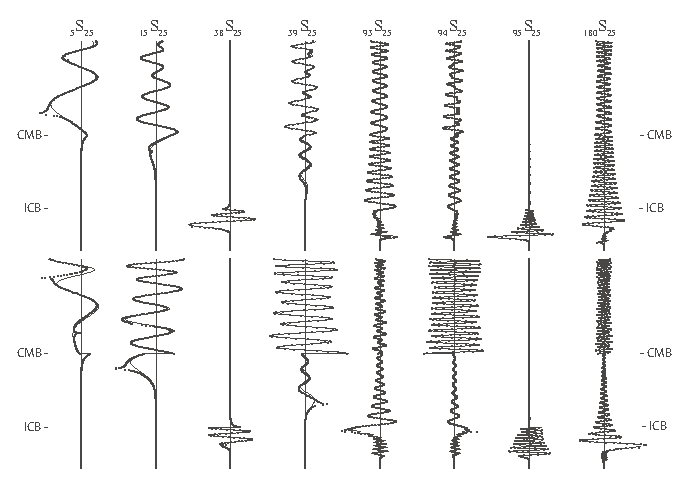
\includegraphics{../figures/chap12/fig19.eps}
}
\end{center}
\caption[U,V Comparison]{\label{12.fig.UVcomp}
几个${}_n{\rm S}_{25}$球型模式的精确({\em 实线\/})与渐近({\em 点线\/})本征函数。({\em 上行\/})径向位移$U$。({\em 下行\/})切向位移$V$。垂直轴从$r=0$延伸至$r=a$,图中标出了核幔边界(CMB)和内核边界(ICB)的位置。渐近近似结果在远离各个折返点$R_{\rm P}$、
$R_{\rm S}$、$R_{\rm K}$、$R_{\rm I}$ 和 $R_{\rm J}$的地方都很精确。(由L. Zhao提供)
}
\end{figure}
\begin{figure}[!b]
\begin{center}
\scalebox{0.95}{
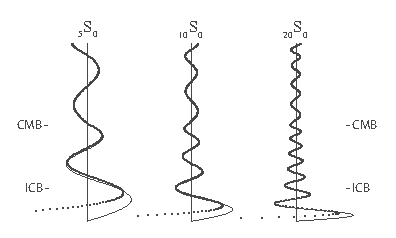
\includegraphics{../figures/chap12/fig20.eps}
}
\end{center}
\caption[U Rad Comparison]{\label{12.fig.Uradcom}
径向模式${}_5{\rm S}_0$,
${}_{10}{\rm S}_0$ 和 ${}_{20}{\rm S}_0$的精确({\em 实线\/})与渐近({\em 点线\/})本征函数$U$。垂直轴从$r=0$延伸至$r=a$,图中标出了核幔边界 (CMB)和内核边界(ICB)的位置。(由L. Zhao提供)
}
\end{figure}
例如区间V中的模式${}_{15}{\rm S}_{25}$,它由折返的P波、${\rm ScS}_{\rm SV}$波和折返的SKS波构成,它的切向位移$V$在地幔中$r=R_{\rm P}$和液态外核中$r=R_{\rm K}$两个半径处发散。${}_{39}{\rm S}_{25}$ 和 ${}_{94}{\rm S}_{25}$这两个${\rm ScS}_{\rm SV}$等价模式的切向位移分别在外核的$r=R_{\rm K}$和内核的$r=R_{\rm I}$两个半径处发散。模式${}_{38}{\rm S}_{25}$ 和 ${}_{95}{\rm S}_{25}$都是${\rm J}_{\rm SV}$等价的,而模式${}_{93}{\rm S}_{25}$ 和 ${}_{180}{\rm S}_{25}$则都是PKIKP等价的。对于这些各式各样的高频模式,渐近表达式对它们的振荡以及瞬逝区域的细节的捕捉程度是惊人的。图~\ref{12.fig.Uradcom}比较了区间X中几个径向模式的渐近与精确本征函数。除了在地心处一致性都很好,在地心处$U$以$r^{-1}$发散,因为相应的$p=0$的射线在那里“折返”。
\index{mode-ray duality!spheroidal modes|)}%

\renewcommand{\thesection}{$\!\!\!\raise1.3ex\hbox{$\star$}\!\!$
\arabic{chapter}.\arabic{section}}
\section{渐近结果点滴}
\renewcommand{\thesection}{\arabic{chapter}.\arabic{section}}

我们可以用前面得到的结果来增进我们对模式的能量平衡以及群速度的认识,还可以推导代表本征频率对球对称地球的模型参数的一阶依赖性的Fr\'{e}chet积分核的渐近表达式。为方便起见,我们在以下讨论中把公式~(\ref{12.geneif})中零点为本征频率的函数表示为
\eq
f=\sum_{\nu}A_{\nu}\sin\half\Psi_{\nu}\qquad
\mbox{or}\qquad f=\sum_{\nu}A_{\nu}\cos\half\Psi_{\nu}.
\en
本节中大部分结果来自 \textcite{zhao&dahlen95b}.

\renewcommand{\thesubsection}{$\!\!\!\raise1.3ex\hbox{$\star$}\!\!$
\arabic{chapter}.\arabic{section}.\arabic{subsection}}
\subsection{P波与S波能量}
\index{energy!P-wave|(}%
\index{energy!S-wave|(}%
\index{P-wave energy|(}%
\index{S-wave energy|(}%
\index{compressional-wave energy|(}%
\index{shear-wave energy|(}%
\renewcommand{\thesubsection}{\arabic{chapter}.\arabic{section}.\arabic{subsection}}

公式~(\ref{12.normal2})中将区间III中球型模式的动能表示成P波和S波的部分能量之和这一结果可以很容易地推广到其它区间。在每一个区间,我们将本征函数$U$和$V$的JWKB渐近表达式代入归一化关系~(\ref{12.normal}),然后将对应于不同振荡波类型的项分离。经过这一过程,结果总能写成如下形式
\eq \label{12.enbal}
\sum_{\nu}f_{\nu}=1,
\en
其中
\eq \label{12.enbal2}
f_{\nu}=\frac{(\p\hspace{-0.3 mm}f/\p\Psi_{\nu})T_{\nu}}
{\sum_{\nu'}(\p\hspace{-0.3 mm}f/\p\Psi_{\nu'})T_{\nu'}}.
\en
这里$f_{\nu}$是类型为$\nu$的波的{\em 动能占比\/}。
\index{energy!fractional}%
\index{fractional energy}%
很容易验证公式~(\ref{12.enbal2})与前面由折返P和SV波相长干涉形成的区间III中模式的结果~(\ref{12.fdef1})--(\ref{12.fdef2})是一致的。对于由最多类型的反射与折返波形成的区间IX中的模式则有
\eq \label{12.enbal3}
f_{\rm PcP}+f_{\rm ScS}+f_{\rm KiK}+f_{\rm I}+f_{\rm J}=1.
\en
~(\ref{12.UGLY})中给出了函数$f$的表达式,通过对$f$求导可以得到五种波的能量占比$f_{\rm PcP}$、$f_{\rm ScS}$、$f_{\rm KiK}$、
$f_{\rm I}$ 和 $f_{\rm J}$。
~(\ref{12.enbal3})中的结果在介质微弱差别近似$\grave{P}\hspace{-0.4 mm}\acute{P}\approx\grave{K}\hspace{-0.4 mm}\acute{K}\approx 0$ 下可以简化很多,此时${\rm ScS}_{\rm SV}$模式有$f_{\rm ScS}\approx 1$而${\rm J}_{\rm SV}$模式有$f_{\rm J}\approx 1$。PKIKP模式则有
\eq \label{12.enbal4}
f_{\rm PcP}\approx\frac{T_{\rm PcP}}{T_{\rm PKIKP}},\qquad
f_{\rm KiK}\approx\frac{T_{\rm KiK}}{T_{\rm PKIKP}},\qquad
f_{\rm I}\approx\frac{T_{\rm I}}{T_{\rm PKIKP}};
\en
即三种压缩波的能量占比就是它们在各自区域的分数走时。这一直觉上很诱人的近似也适用于区间X中的径向模式。~(\ref{12.enbal})中的渐近能量平衡对于环型模式变得没有必要,因为SH模式有$f_{\rm S}=1$,ScS模式有$f_{\rm ScS}=1$,J模式有$f_{\rm J}=1$。
\index{energy!P-wave|)}%
\index{energy!S-wave|)}%
\index{P-wave energy|)}%
\index{compressional-wave energy|)}%
\index{shear-wave energy|)}%
\index{S-wave energy|)}%

\renewcommand{\thesubsection}{$\!\!\!\raise1.3ex\hbox{$\star$}\!\!$
\arabic{chapter}.\arabic{section}.\arabic{subsection}}
\subsection{群速度}
\index{group speed|(}%
\index{speed!group|(}%
\renewcommand{\thesubsection}{\arabic{chapter}.\arabic{section}.\arabic{subsection}}

要计算一个模式的渐近群速度,我们将相长干涉关系~(\ref{12.geneif})看作是如下形式的方程
\eq \label{12.feq0}
f(\omega,p)=f(\omega,k/\omega)=0,
\en
其中$k=l+\half$是渐近波数。用链式法则将以上方程对$\omega$和 $k$求导,我们得到
\eq \label{12.group}
C=\frac{d\omega}{dk}=
-\frac{1}{\om}\left(\frac{\p\hspace{-0.3 mm}f}{\p p}\right)
\left(\frac{\p\hspace{-0.3 mm}f}{\p\omega}
-\frac{p}{\omega}\frac{\p\hspace{-0.3 mm}f}{\p p}
\right)^{-1}.
\en
对于环型模式,$f=\sin\half\Psi$,其中$\Psi$代表$\Psi_{\rm S}$、 $\Psi_{\rm ScS}$或 $\Psi_{\rm J}$其中之一,因而
\eq \label{12.torgrp}
\frac{\p\hspace{-0.3 mm}f}{\p\omega}
=\half\tau\cos\half\Psi,\qquad
\frac{1}{\om}\frac{\p\hspace{-0.3 mm}f}{\p p}
=-\half\Theta\cos\half\Psi,
\en
这里我们使用了射线理论关系式$d\tau/dp=-\Theta$。将~(\ref{12.torgrp})代入~(\ref{12.group}),利用$T=\tau+p\Theta$,我们看到一个环型模式的群速度就是震中距与走时的比值:
\eq \label{12.group2}
C=\Theta\hspace{-0.2 mm}/T.
\en
将这一物理上很诱人的结果与同一模式所对应的相速度$c=p^{-1}$的公式做比较是很有意义的:
\eq \label{group3}
c=d\Theta\hspace{-0.2 mm}/\hspace{-0.2 mm}dT.
\en
相速度$c$所代表的是形成一个模式的相长干涉的SH, ${\rm ScS}_{\rm SH}$ 或 ${\rm J}_{\rm SH}$波前进中的{\em 视\/}角速率,
\index{phase speed}%
\index{speed!phase}%
而群速度$C$则是它们的{\em 绝对\/}角速率。
\index{group speed}%
\index{speed!group}%
值得注意的是$C$仅仅依赖于射线参数$p$,这意味着环型模式频散曲线图中在$\om=ck$斜线上的所有模式的群速度$C$是相同的。对图~\ref{fig:tormodefreqs}做一个简单的视觉检视可以看出的确如此。方程~(\ref{12.group2})的推导也可以通过把表12.3中的JWKB本征函数代入精确表达式~(\ref{11.Lgrvel}),再利用Riemann-Lebesgue公理来计算其中的积分。或者更简单地,直接对环型模式本征频率的显式方程$\omega\tau(k/\omega)={\rm constant}$求导。

对于球型模式的表达式$f=\sum_{\nu}A_{\nu}\sin\half\Psi_{\nu}$
或 $f=\sum_{\nu}A_{\nu}\cos\half\Psi_{\nu}$,我们发现
\eq
\frac{\p\hspace{-0.3 mm}f}{\p\omega}=
\sum_{\nu}\left(\frac{\p\hspace{-0.3 mm}f}{\p
\Psi_{\nu}}\right)\tau_{\nu},\qquad
\frac{1}{\om}\frac{\p\hspace{-0.3 mm}f}{\p p}
=-\sum_{\nu}\left(\frac{\p\hspace{-0.3 mm}f}
{\p \Psi_{\nu}}\right)\Theta_{\nu},
\en
上式精确到$\omega^{-1}$。将这些关系代入方程~(\ref{12.group}),再利用定义~(\ref{12.enbal2}),我们发现
\eq \label{12.group4}
C=\sum_{\nu}f_{\nu}(\Theta_{\nu}/\hspace{0.1 mm}T_{\nu}),
\en
这是~(\ref{12.group2})中的基本结果的推广。方程~(\ref{12.group4})显示,普遍来讲一个模式的渐近群速度是构成该模式的波的各自群速度$\Theta_{\nu}/T_{\nu}$的{\em 加权平均\/}。{\em 动能占比\/}$f_{\nu}$作为权重因子是很合理的,
\index{energy!fractional}%
\index{fractional energy}%
因为一个波的能量是以群速度传播的。(\ref{12.group4})的结果也可以通过将每一个球型模式区间的JWKB渐近本征函数$U$和 $V$代入群速度的精确积分表达式~(\ref{11.Rgrvel})中得到。区间III中的地幔球型模式的群速度为$C=f_{\rm P}(\Theta_{\rm P}/T_{\rm P})
+f_{\rm S}(\Theta_{\rm S}/T_{\rm S})$,而区间IX的全球模式群速度则为
\eqa \label{12.group5} \lefteqn{
C=f_{\rm PcP}(\Theta_{\rm PcP}/T_{\rm PcP})
+f_{\rm ScS}(\Theta_{\rm ScS}/T_{\rm ScS})} \nonumber \\
&&\mbox{}\qquad+f_{\rm KiK}(\Theta_{\rm KIK}/T_{\rm KIK})
+f_{\rm I}(\Theta_{\rm I}/T_{\rm I})
+f_{\rm J}(\Theta_{\rm J}/T_{\rm J}).
\ena
(\ref{12.group5})这一结果还可以在$\grave{P}\hspace{-0.3 mm}\acute{P}
\approx\grave{K}\hspace{-0.3 mm}\acute{K}\approx 0$ 这一地震学感兴趣的情形做简化,此时${\rm ScS}_{\rm SV}$模式有$C\approx\Theta_{\rm ScS}/T_{\rm ScS}$,${\rm J}_{\rm SV}$模式有$C\approx\Theta_{\rm J}/T_{\rm J}$,PKIKP模式有$C\approx\Theta_{\rm PKIKP}/T_{\rm PKIKP}$。对于径向模式,由于对应的波正好穿过地心,$\Theta_{\rm PKIKP}=\pi$。射线参数$p$相同的球型模式并不都具有相同的群速度,因为分数动能$f_{\nu}$强烈依赖于模式的种类
\index{group speed|)}%
\index{speed!group|)}%

\renewcommand{\thesubsection}{$\!\!\!\raise1.3ex\hbox{$\star$}\!\!$
\arabic{chapter}.\arabic{section}.\arabic{subsection}}
\subsection{Fr\'{e}chet 积分核}
\index{Fr\'{e}chet kernel!asymptotic|(}%
\renewcommand{\thesubsection}{\arabic{chapter}.\arabic{section}.\arabic{subsection}}

环型与球型模式的渐近Fr\'{e}chet积分核的推导可以用类似的方式,将相长干涉关系~(\ref{12.feq0})改写为如下形式
\eq \label{12.feq02}
f(\om,k\hspace{-0.1 mm}/\hspace{0.1 mm}\om;\alpha,\beta,d)=0,
\en
其中的自变$\alpha$、$\beta$ 和 $d$显示了对压缩与剪切波速度以及不连续面的半径$c$、$b$和 $a$的依赖性。对上式求一阶变分,保持波数$k$不变,我们得到
\eqa \label{12.Frech}
\lefteqn{\delta\om=-\left[\left(
\frac{\p\hspace{-0.3 mm}f}{\p\alpha}\right)\delta\hspace{-0.1 mm}\alpha
+\left(\frac{\p\hspace{-0.3 mm}f}{\p\beta}\right)\delta\hspace{-0.2 mm}\beta
+\left(\frac{\p\hspace{-0.3 mm}f}{\p d}\right)\delta\hspace{-0.1 mm}d\right]
} \nonumber \\
&&\mbox{}\times\left(\frac{\p\hspace{-0.3 mm}f}{\p\omega}
-\frac{p}{\omega}\frac{\p\hspace{-0.3 mm}f}{\p p}\right)^{-1}.
\ena
方程~(\ref{12.Frech})给出了由于地球模型参数的微小扰动$\delta\hspace{-0.1 mm}\alpha$、
$\delta\hspace{-0.2 mm}\beta$和$\delta\hspace{-0.1 mm}d$而导致的模式${}_n{\rm T}_l$ 或 ${}_n{\rm S}_l$的本征频率的一阶扰动$\delta\om$。由于压缩与剪切波速度是出现在公式~(\ref{12.feq02})中相位积分$\Psi_{\nu}$的被积函数里,变分表达式$(\p\hspace{-0.3 mm}f\hspace{-0.3 mm}/\hspace{-0.3 mm}
\p\alpha)\,\delta\hspace{-0.1 mm}\alpha$
和 $(\p\hspace{-0.3 mm}f\hspace{-0.3 mm}/\hspace{-0.3 mm}
\p\beta)\,\delta\hspace{-0.2 mm}\beta$仅仅是象征性的。

为展示如何使用(\ref{12.Frech}),我们首先考虑一个SH等价的环型模式,该模式有$f=\sin(\om\int_{R_{\rm S}}^aq_{\beta}\,dr-\pi/4)$。
对其求相对于剪切波速$\beta$和半径$a$的偏微分,我们得到
\eq \label{12.Frech2}
\delta\om=2\om T_{\rm S}^{-1}\int_{R_{\rm S}}^a
\beta^{-3}q_{\beta}^{-1}\delta\hspace{-0.2 mm}\beta\,dr
-2\om T_{\rm S}^{-1}q_{\beta}(a)\,\delta\hspace{-0.1 mm}a.
\en
我们可以用第9章引入的符号将上式改写为
\eq \label{12.chap9}
\delta\om=\int_0^a(\delta\hspace{-0.2 mm}\alpha\,K_{\alpha}
+\delta\hspace{-0.3 mm}\beta\,K_{\beta})\,dr+\sum_d\delta\hspace
{-0.1 mm}d\,[K_d]^+_-,
\en
其中$K_{\alpha}=0$,且
\eq
K_{\beta}=\left\{\begin{array}{ll}
2\om T_{\rm S}^{-1}\beta^{-3}q_{\beta}^{-1}, & \quad R_{\rm S}\ll r\leq a \\
\vspace{-1.5 mm} & \vspace{-1.5 mm} \\
0, & \quad 0\leq r\ll R_{\rm S}, \end{array}\right.
\en
\eq
[K_a]^+_-=-2\om T_{\rm S}^{-1}q_{\beta}(a),\qquad
[K_b]^+_-=[K_c]^+_-=0.
\en
对于一个${\rm ScS}_{\rm SH}$等价模式,其非零的Fr\'{e}chet积分核为
\eq
K_{\beta}=\left\{\begin{array}{ll}
2\om T_{\rm ScS}^{-1}\beta^{-3}q_{\beta}^{-1}, & \quad b+\leq r\leq a \\
\vspace{-1.5 mm} & \vspace{-1.5 mm} \\
0, & \quad 0\leq r\leq b-, \end{array}\right.
\en
\eq
[K_a]^+_-=-2\om T_{\rm ScS}^{-1}q_{\beta}(a),\qquad
[K_b]^+_-=2\om T_{\rm ScS}^{-1}q_{\beta}(b+).
\en
对于一个SH等价振荡模式,其渐近剪切波速积分核$K_{\beta}$在折返点$r=R_{\rm S}$上方以$q_{\beta}^{-1}$的形式发散,而在折返半径以下恒为零。一个${\rm ScS}_{\rm SH}$等价模式对核幔边界的半径$r=b$以及自由表面的半径$r=a$均有敏感性。

区段III中地幔球型模式所有的非零的Fr\'{e}chet积分核为
\eq
K_{\alpha}=\left\{\begin{array}{ll}
2\om f_{\rm P}T_{\rm P}^{-1}\alpha^{-3}
q_{\alpha}^{-1}, & \quad R_{\rm P}\ll r\leq a \\
\vspace{-1.5 mm} & \vspace{-1.5 mm} \\
0, & \quad 0\leq r\ll R_{\rm P}, \end{array}\right.
\en
\eq
K_{\beta}=\left\{\begin{array}{ll}
2\om f_{\rm S}T_{\rm S}^{-1}\beta^{-3}
q_{\beta}^{-1}, & \quad R_{\rm S}\ll r\leq a \\
\vspace{-1.5 mm} & \vspace{-1.5 mm} \\
0, & \quad 0\leq r\ll R_{\rm S}, \end{array}\right.
\en
\eq
[K_a]^+_-=-2\om [f_{\rm P}T_{\rm P}^{-1}q_{\alpha}(a)
+f_{\rm S}T_{\rm S}^{-1}q_{\beta}(a)],
\en
而区段IX中的全球模式的积分核为
\eq \label{12.Frech3}
K_{\alpha}=\left\{\begin{array}{ll}
2\om f_{\rm PcP}T_{\rm PcP}^{-1}\alpha^{-3}
q_{\alpha}^{-1}, & \vspace{0.5 mm}\quad b+\leq r\leq a \\
\vspace{-1.5 mm} & \vspace{-1.5 mm} \\
2\om f_{\rm KiK}T_{\rm KiK}^{-1}\alpha^{-3}
q_{\alpha}^{-1}, & \vspace{0.5 mm}\quad c+\leq r\leq b- \\
\vspace{-1.5 mm} & \vspace{-1.5 mm} \\
2\om f_{\rm I}T_{\rm I}^{-1}\alpha^{-3}
q_{\alpha}^{-1}, & \vspace{0.5 mm}\quad R_{\rm I}\ll r\leq c- \\
\vspace{-1.5 mm} & \vspace{-1.5 mm} \\
0, & \vspace{0.5 mm}\quad 0\leq r\ll R_{\rm I},
\end{array}\right.
\en
\eq
K_{\beta}=\left\{\begin{array}{ll}
2\om f_{\rm ScS}T_{\rm ScS}^{-1}\beta^{-3}
q_{\beta}^{-1}, & \quad b+\leq r\leq a \\
\vspace{-1.5 mm} & \vspace{-1.5 mm} \\
0, & \quad c+\leq r\leq b- \\
\vspace{-1.5 mm} & \vspace{-1.5 mm} \\
2\om f_{\rm J}T_{\rm J}^{-1}\beta^{-3}
q_{\beta}^{-1}, & \quad R_{\rm J}\ll r\leq c- \\
\vspace{-1.5 mm} & \vspace{-1.5 mm} \\
0, & \quad 0\leq r\ll R_{\rm J}, \end{array}\right.
\en
\eq
[K_a]^+_-=-2\om [f_{\rm PcP}T_{\rm PcP}^{-1}q_{\alpha}(a)
+f_{\rm ScS}T_{\rm ScS}^{-1}q_{\beta}(a)],
\en
\eqa \lefteqn{
[K_b]^+_-=2\om [f_{\rm PcP}T_{\rm PcP}^{-1}q_{\alpha}(b+)} \nonumber \\
&&\mbox{}\qquad\qquad+f_{\rm ScS}T_{\rm ScS}^{-1}q_{\beta}(b+)
-f_{\rm KiK}T_{\rm KiK}^{-1}q_{\alpha}(b-)],
\ena
\eqa \label{12.Frech4} \lefteqn{
[K_c]^+_-=2\om [f_{\rm KiK}T_{\rm KiK}^{-1}q_{\alpha}(c+)} \nonumber \\
&&\mbox{}\qquad\qquad\qquad-f_{\rm I}T_{\rm I}^{-1}
q_{\beta}(c-)-f_{\rm J}T_{\rm J}^{-1}q_{\alpha}(c-)].
\ena
\begin{figure}[!b]
\begin{center}
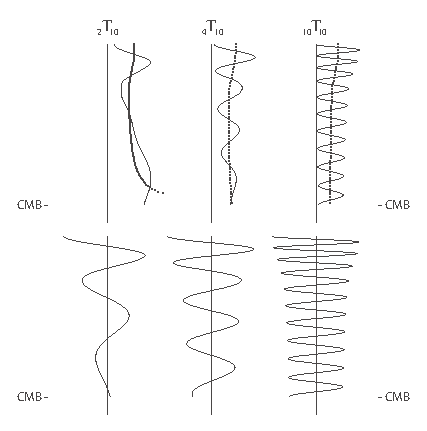
\includegraphics{../figures/chap12/fig21.eps}
\end{center}
\caption[Tor Frech Comp]{\label{12.fig.Frechet}
几个$l=10$的环型振荡的精确({\em 实线\/})与渐近({\em 点线\/})Fr\'{e}chet积分核。({\em 上行\/})剪切波速积分核$K_{\beta}$。({\em 下行\/})密度积分核$K_{\rho}^{\prime}$。垂直轴是去掉地壳的1066A模型中从地表向下的深度。图中标出了核幔边界(CMB)的位置。模式${}_2{\rm T}_{10}$是一个SH等价模式,在下地幔$r=R_{\rm S}$处有一个折返点。而模式${}_4{\rm T}_{10}$ 和 ${}_{10}{\rm T}_{10}$是${\rm ScS}_{\rm SH}$等价模式,它们没有折返点。渐近的剪切波速积分核在$r=R_{\rm S}$之上均为正,而渐近密度积分核则处处为零。(由L. Zhao提供)
}
\end{figure}
同样地,(\ref{12.Frech3})--(\ref{12.Frech4})中的结果在$\grave{P}\hspace{-0.4 mm}\acute{P}
\approx\grave{K}\hspace{-0.4 mm}\acute{K}\approx 0$ 时可以进一步简化。例如,PKIKP模式的渐近Fr\'{e}chet积分核简化为$K_{\beta}\approx 0$以及
\eq
K_{\alpha}\approx\left\{\begin{array}{ll}
2\om T_{\rm PKIKP}^{-1}\alpha^{-3}q_{\alpha}^{-1},
& \quad R_{\rm I}\ll r\leq a \\
\vspace{-1.5 mm} & \vspace{-1.5 mm} \\
0, & \quad 0\leq r\ll R_{\rm I}, \end{array}\right.
\en
\eq
K_d\approx 2\om T_{\rm PKIKP}^{-1}q_{\alpha}(d).
\en
\begin{figure}[!t]
\begin{center}
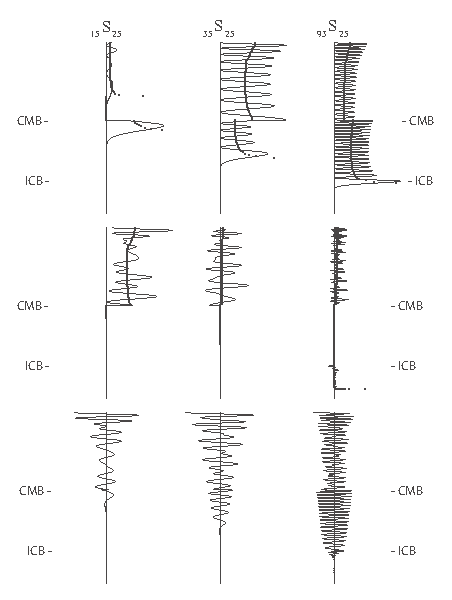
\includegraphics{../figures/chap12/fig22.eps}
\end{center}
\caption[Spher Frech Comp]{\label{12.fig.Frechet2}
几个$l=25$的球型振荡的精确({\em 实线\/})与渐近({\em 点线\/})Fr\'{e}chet积分核。({\em 顶行\/})压缩波速积分核$K_{\alpha}$。({\em 中行\/})剪切波速积分核$K_{\beta}$。({\em 下行\/})密度积分核$K_{\rho}^{\prime}$。垂直轴在去掉地壳的1066A模型中从地表向下延伸到地心。图中标出了核幔边界(CMB)和内核边界(ICB)的位置。模式${}_{15}{\rm S}_{25}$是一个${\rm ScS}_{\rm SV}$-SKS等价模式,模式${}_{35}{\rm S}_{25}$是一个PKP等价模式,模式${}_{93}{\rm S}_{25}$是一个PKIKP等价模式。渐近的波速积分核在相应折返点$r=R$之上均为正,而渐近密度积分核则处处为零。(由L. Zhao提供)
}
\end{figure}
在这一低阻抗近似下,径向模式有$K_{\alpha}\approx
2\om T_{\rm PKIKP}^{-1}\alpha^{-2}$ 和
$K_d\approx 2\om T_{\rm PKIKP}^{-1}\alpha_{\rm d}^{-1}$。

值得注意的是渐近本征频率并不依赖于地球模型中的密度$\rho$分布,所有模式的密度积分核$K_{\raisebox{0.3 ex}{\scriptsize$\rho$}}^{\prime}$均恒为零。对密度的渐近依赖性只有在按频率倒数$\om^{-1}$的展开式的下一项才会出现。有意思的是,那时出现的是密度的{\em 梯度\/}$\dot{\rho}$而不是密度本身,这与我们在第9.3节中对密度依赖性的讨论一致。总的来讲,渐近Fr\'{e}chet积分核$K_{\alpha}$、$K_{\beta}$和
$K_{\raisebox{0.3 ex}{\scriptsize$\rho$}}^{\prime}$与对应的精确积分核的“移动平均”之间有很好的一致性,如图~\ref{12.fig.Frechet}中的几个环型模式和图~\ref{12.fig.Frechet2}中的几个球型模式所示。作为另外一种推导方法,我们可以把JWKB渐近本征函数代入Fr\'{e}chet积分核的精确表达式中,这样会使这一结果更明确,因为在用Riemann-Lebesgue公理计算积分时所有振荡函数的平方项都被$\half$取代。渐近结果所建立的前提是地球的结构在不连续面之间的径向变化足够光滑而允许做这种平均,这也解决了两组积分核在分辨度上的明显的不一致。在$\omega^{-1}$的最低阶,高频简正模式与体波走时对地球内部结构所做的约束本质上是完全一样的。
\index{Fr\'{e}chet kernel!asymptotic|)}%

\renewcommand{\thesubsection}{$\!\!\!\raise1.3ex\hbox{$\star$}\!\!$
\arabic{chapter}.\arabic{section}.\arabic{subsection}}
\subsection{压缩与剪切能量}
\index{energy!compressional|(}%
\index{energy!shear|(}%
\index{compressional energy|(}%
\index{shear energy|(}%
\renewcommand{\thesubsection}{\arabic{chapter}.\arabic{section}.\arabic{subsection}}

球型模式的压缩与剪切的能量占比定义为
\index{fractional energy}%
\index{energy!fractional}%
\eq
f_{\kappa}=2\om^{-1}\int_0^a\kappa K_{\kappa}\,dr,\qquad
f_{\mu}=2\om^{-1}\int_0^a\mu K_{\mu}\,dr,
\en
其中
\eq
K_{\kappa}=(2\rho\alpha)^{-1}K_{\alpha},\qquad
K_{\mu}=(2\rho\beta)^{-1}K_{\beta}+\fourthirds
(2\rho\alpha)^{-1}K_{\alpha}.
\en
代入$K_{\alpha}$ 和 $K_{\beta}$的渐近表达式,我们发现区间III的地幔模式有
\eq \label{12.csener}
f_{\kappa}\approx \fiveninths f_{\rm P},\qquad
f_{\mu}\approx \fourninths f_{\rm P}+f_{\rm S},
\en
而区间IX的全球模式有
\eq
f_{\kappa}\approx \fiveninths f_{\rm PcP}+f_{\rm KiK}
+\fiveninths f_{\rm I},
\en
\eq \label{12.csener2}
f_{\mu}\approx \fourninths f_{\rm PcP}+f_{\rm ScS}
+\fourninths f_{\rm I}+f_{\rm J}.
\en
为简化~(\ref{12.csener})--(\ref{12.csener2})中的结果,我们在地球模型的固态区域使用了泊松近似$\alpha^2\approx 3\beta^2$。值得注意的是压缩与剪切波分数能量的和为1:
\eq
f_{\kappa}+f_{\mu}\approx 1,
\en
这是无重力地球模型中可以预期的。在$\grave{P}\hspace{-0.4 mm}\acute{P}
\approx\grave{K}\hspace{-0.4 mm}\acute{K}\approx 0$时, 的情形下,${\rm ScS}_{\rm SV}$ 和 ${\rm J}_{\rm SV}$模式均有$f_{\kappa}\approx 0$ and $f_{\mu}\approx 1$,而PKIKP或径向模式则有
\eq
f_{\kappa}\approx T_{\rm PKIKP}^{-1}
(\fiveninths T_{\rm PcP}+T_{\rm KiK}
+\fiveninths T_{\rm I}),
\en
\eq
f_{\mu}\approx T_{\rm PKIKP}^{-1}
(\fourninths T_{\rm PcP}
+\fourninths T_{\rm I})
\en
比例$f_{\kappa}\!:\!f_{\mu}=5/9\!:\!4/9$是均匀泊松介质中平面P波的经典能量分配。
\index{energy!compressional|)}%
\index{energy!shear|)}%
\index{compressional energy|)}%
\index{shear energy|)}%

\renewcommand{\thesubsection}{$\!\!\!\raise1.3ex\hbox{$\star$}\!\!$
\arabic{chapter}.\arabic{section}.\arabic{subsection}}
\subsection{横向各向同性地球模型}
\index{Earth model!transversely isotropic|(}%
\renewcommand{\thesubsection}{\arabic{chapter}.\arabic{section}.\arabic{subsection}}

我们所用来推导SNREI地球中的渐近本质频率与本质函数的所有做法都可以直接推广到横向各向同性地球模型中。第一步是计算传播的P, SV或SH体波的走时$T$、角震中距$\Theta$和截距时间$\tau$。\textcite{woodhouse81b}展示了运动学公式~(\ref{12.DistT})和~(\ref{12.taudef2})必须换成更普遍的公式
\eq \label{12.ti}
T=2\int_R^aq_T\,dr,\qquad \Theta=2\int_R^aq_{\Theta}\,dr,
\qquad\tau=2\int_R^aq_{\tau}\,dr,
\en
其中积分限需要改变来考虑反射波而不是折返波、多个射线段以及射线端点不在表面的情况。对于一个SH波,被积函数$q_T$、$q_{\Theta}$ 和 $q_{\tau}$分别为
\begin{displaymath}
q_T=\frac{(\beta_{\rm h}\beta_{\rm v})^{-1}}
{\sqrt{\beta_{\rm h}^{-2}-p^2r^{-2}}},\qquad
q_{\Theta}=\frac{(\beta_{\rm h}/\hspace{-0.3 mm}\beta_{\rm v})pr^{-2}}
{\sqrt{\beta_{\rm h}^{-2}-p^2r^{-2}}},
\end{displaymath}
\eq \label{12.ti2}
q_{\tau}=q_T-pq_{\Theta}=(\beta_{\rm h}/\hspace{-0.3 mm}\beta_{\rm v})
\sqrt{\beta_{\rm h}^{-2}-p^2r^{-2}},
\en
其中$\beta_{\rm h}$ 和 $\beta_{\rm v}$分别为\textcolor{red}{水平和垂直}方向的波速。射线参数为$p$的SH波的折返半径为$R_{\rm S}=p\beta_{\rm h}$。在~(\ref{12.ti2})中出现在平方根中的是$\beta_{\rm h}$而不是$\beta_{\rm v}$是很自然的,因为波在折返时的传播方向是水平的。很明显,(\ref{12.ti})--(\ref{12.ti2})中的结果在各向同性地球中退化为~(\ref{12.DistT})和~(\ref{12.taudef2}),其中的$\beta_{\rm h}=\beta_{\rm v}=\beta$。对于P和SV波,$q_T$、 $q_{\Theta}$ 和$q_{\tau}$的公式更复杂,但是在横向各向同性地球中,$p=dT\hspace{-0.2 mm}/\hspace{-0.2 mm}d\Theta$ 
和$d\tau\hspace{-0.2 mm}/\hspace{-0.2 mm}dp=-\Theta$这两个重要关系仍保持成立。

\textcite{mochizuki92}对横向各向同性地球中环型模式的方程和边界条件进行了渐近分析。他展示了表~\ref{table:SH}中的渐近本质频率仍然成立,但是$\tau_{\rm S}$、$\tau_{\rm ScS}$ 和 $\tau_{\rm J}$必须用~(\ref{12.ti})--(\ref{12.ti2})而不是~(\ref{12.taudef2})来计算,而且区分SH波的四个区间的射线参数是由水平传播速度$\beta_{\rm h}$确定的。要建立表~\ref{12.table.toreifs}中的渐近本征函数,除了要重新计算走时$T_{\rm S}$、$T_{\rm ScS}$和 $T_{\rm J}$以外,还必须把$q_{\beta}$换成$q_{\tau}$,把刚度$\mu$换成横向各向同性参数$L$。\textcite{mochizuki94}也考虑了更复杂的P-SV情形,他忽略了内核与外核,仅仅得到了区间III中的地幔球型模式的结果。这些模型的渐近本质频率关系具有~(\ref{12.freqIII})的形式,只是$\Psi_{\rm P}$ 
和$\Psi_{\rm S}$要用~(\ref{12.ti})--(\ref{12.ti2})来计算,而且$\acute{S}\hspace{-0.4 mm}\grave{S}$ 要被一个依赖于横向各向同性弹性参数$C$、$A$、$L$、$N$ 和 $F$的广义反射系数取代。有意愿的话,其它区间的模式的类似结果也可以用上述方法得到。
\index{Earth model!transversely isotropic|)}%

\section{体波响应}
\index{body-wave response|(}%
\index{response!body-wave|(}%
\label{12.sec.Green}

到此为止,我们仅仅考虑了模式与射线之间二象性的第一个方面,也就是将地球的自由振荡表示成相长干涉的体波的叠加。在最后这一节,我们来讨论第二个方面,即“从模式到射线”的反问题。我们将证明,SNREI地球响应的环型与球型简正模式叠加的表达式在$\om\rightarrow\infty$的极限下等价于多次反射与折射的SH和P-SV波的叠加。我们用简单的步骤来达到这一从模式叠加到射线叠加的变换,完整详细地讨论简单的SH波,对P-SV波则仅给出最终结果。在第15章中,通过将JWKB近似系统性地用于无重力的运动方程$-\om^2\!\rho\hspace{0.3 mm}\bs-\bdel\cdot\bT=\bzero$,其中$\bT=\kappa(\bdel\cdot\bs)\bI+2\mu\bd$,我们将本节得到的射线理论响应推广到横向不均匀地球。

\subsection{SH 格林张量}
\index{Green tensor!SH|(}%
\index{tensor!SH Green|(}%

我们分析的出发点是频率域格林张量的行波表达式,公式~(\ref{eq:11.repre3})。我们忽略衰减,令沿所有频散曲线分支的衰减率$\gamma_n(k)$为零。同时,为简洁起见,我们仅关注$s=1$的传播小于半个地球周长的波。基于这些前提,我们可以将{\em 精确的\/}SH波格林张量$\bG_{\rm SH}(\bx,\bx';\om)$写成如下形式
\eqa \label{12.Green} \lefteqn{
\bG=\frac{1}{2\pi}(\brh\times\bdel_{\!1})
(\brh'\times\bdel_{\!1}^{\prime})
\sum_{n=0}^{\infty}\int_{-\infty}^{\infty}
\left(\frac{W_nW_n^{\prime}}{\om_n^2-\om^2}\right)} \nonumber \\
&&\mbox{}\qquad\qquad\qquad\times
Q_{k-\subhalf}^{(1)}(\cos\Theta)\,k^{-1}dk,
\ena
其中$\Theta={\rm arccos}\,(\brh\cdot\brh')$是角震中距,撇号表示在震源点$\bx'$处取值。为便于向体波表达式的变换,我们将积分变量从波数$k$变为射线参数$p$。在{\em 固定径向阶数 n\/}时,这两者之间的关系为$k^{-1}dk=(1-C/c)^{-1}p^{-1}dp$,其中$C=d\om\hspace{-0.3 mm}/\hspace{-0.3 mm}dk$与$c=\om\hspace{-0.2 mm}/\hspace{-0.2 mm}k$分别为群速度与相速度。在做此坐标变换之后,我们交换求和与积分顺序得到
\eqa \label{12.Green2} \lefteqn{
\bG=\frac{1}{2\pi}(\brh\times\bdel_{\!1})
(\brh'\times\bdel_{\!1}^{\prime})
\int_{-\infty}^{\infty}\sum_{n=0}^{\infty}\left(
\frac{W_nW_n^{\prime}}{\om_n^2-\om^2}\right)} \nonumber \\
&&\mbox{}\qquad\qquad\qquad\times Q_{\omega p-\subhalf}^{(1)}
(\cos\Theta)\,(1-C/c)^{-1}\,p^{-1}dp.
\ena
(\ref{12.Green2})中的积分路径是紧贴着实$p$轴下方。为具体化,我们假定角频率为正,即$\om>0$。实部为正的射线参数$\Re{\rm e}\,p>0$与实部为负的射线参数$\Re{\rm e}\,p<0$分别对应于沿$\Theta$增加与减小的方向传播的波。

下一步是将本质频率$\om_n$及相应的接收点和震源的本征函数$W_n$和$W_n^{\prime}$的JWKB渐近表达式代入公式~(\ref{12.Green2}),然后对径向阶数$n$求和。这样的求和是对{\em 固定的射线参数 p\/},因此所有需要考虑的模式都在同一个区间。${\rm J}_{\rm SH}$内核模式不会被地幔中的点源所激发,因此我们仅仅需要考虑两个求和,对区段II中的折返SH模式,以及对区段III中的${\rm ScS}_{\rm SH}$模式。对于${\rm ScS}_{\rm SH}$模式,方便的做法是定义三个径向慢度的积分$X$, $X'$ 和 $\overline{X}$
\begin{displaymath}
\om X=\om\int_b^rq\,dr+\pi/2,\qquad
\om X'=\om\int_b^{r'}q\,dr+\pi/2,
\end{displaymath}
\eq \label{12.threeX}
\om\overline{X}=\om\int_b^aq\,dr=\half\om\tau_{\rm ScS}.
\en
利用表~\ref{table:SH}和表~\ref{12.table.toreifs}中的结果,我们可以将区间III中的径向阶数求和写成
\eqa \label{12.Green3} \lefteqn{
\sum_{n=0}^{\infty}\left(\frac{W_nW_n^{\prime}}{\om_n^2-\om^2}\right)
=4T_{\rm ScS}^{-1}(rr'\beta\beta')^{-1}(\rho\rho' q_{\beta}
q_{\beta}^{\prime})^{-1/2}} \nonumber \\
&&\mbox{}\qquad\qquad\times\sum_{n'=1}^{\infty}\frac{\sin
n'\pi(X/\hspace{0.3 mm}\overline{X})\sin n'\pi
(X'\hspace{-0.4 mm}/\hspace{0.3 mm}\overline{X})}
{(n'\pi/\hspace{0.3 mm}\overline{X})^2-\om^2},
\ena
其中$n'=n+1$。公式~(\ref{12.Green3})中对$n'$的求和有解析结果为
\eqa \label{12.Green4} \lefteqn{
\sum_{n'=1}^{\infty}\frac{\sin
n'\pi(X/\hspace{0.3 mm}\overline{X})\sin n'\pi
(X'\hspace{-0.4 mm}/\hspace{0.3 mm}\overline{X})}
{(n'\pi/\hspace{0.3 mm}\overline{X})^2-\om^2}} \nonumber \\
&&\mbox{}=\frac{\overline{X}}{4\om}
\left[\frac{\cos\om(\overline{X}-(X+X'))
-\cos\om(\overline{X}-|X-X'|)}{\sin\om\overline{X}}\right].
\ena
通过考虑右边表达式中的傅里叶余弦级数,以及用正交性来确定系数的习惯做法可以很容易地验证这一等式。将~(\ref{12.Green4})中的正弦和余弦函数分解为复数指数形式,再用二项式展开,我们可以将~(\ref{12.Green3})中对区段III中${\rm ScS}_{\rm SH}$模式的求和写成
\eqa \label{12.Green5} \lefteqn{
\sum_{n=0}^{\infty}\left(\frac{W_nW_n^{\prime}}{\om_n^2-\om^2}\right)
=\half(i\om)^{-1}(\tau_{\rm ScS}/T_{\rm ScS})(rr'\beta\beta')^{-1}}
\nonumber \\
&&\mbox{}\qquad\qquad\times
(\rho\rho' q_{\beta}q_{\beta}^{\prime})^{-1/2}
\sum_{j=1}^{\infty}\exp(-i\om\tau_j),
\ena
其中
\begin{displaymath}
\tau_1=\left|\int_{r'}^rq\,dr\right|,\qquad
\tau_2=\int_b^{r'}q\,dr+\int_b^rq\,dr,
\end{displaymath}
\begin{displaymath}
\tau_3=\int_{r'}^aq\,dr+\int_r^aq\,dr,\qquad
\tau_4=2\int_b^aq\,dr-\left|\int_{r'}^rq\,dr\right|,
\end{displaymath}
\eq \label{12.tausubnu}
\tau_j=\tau_{j-4}+2\int_b^aq\,dr\quad\mbox{for $j\geq 5$.}
\en
对区段II中折返SH模式的求和可以用相似的方式处理,通过重新定义~(\ref{12.threeX})中的径向慢度积分:
\begin{displaymath}
\om X=\om\int_b^rq\,dr+\pi/4,\qquad
\om X'=\om\int_b^{r'}q\,dr+\pi/4,
\end{displaymath}
\eq
\om \overline{X}=\om\int_{R_{\rm S}}^aq\,dr-\pi/4
=\half(\om\tau_{\rm S}-\pi/2).
\en
我们不是得到公式~(\ref{12.Green5}),而是
\eqa \label{12.Green6} \lefteqn{
\sum_{n=0}^{\infty}\frac{W_nW_n^{\prime}}{\om_n^2-\om^2}
=\half(i\om)^{-1}(\tau_{\rm S}/T_{\rm S})(rr'\beta\beta')^{-1}}
\nonumber \\
&&\mbox{}\qquad\qquad\times
(\rho\rho' q_{\beta}q_{\beta}^{\prime})^{-1/2}
\sum_{j=1}^{\infty}\exp(-i\om\tau_j+iN_j\pi/2),
\ena
其中
\begin{displaymath}
\tau_1=\left|\int_{r'}^rq\,dr\right|,\qquad
\tau_2=\int_{R_{\rm S}}^{r'}q\,dr+\int_{R_{\rm S}}^rq\,dr,
\end{displaymath}
\begin{displaymath}
\tau_3=\int_{r'}^aq\,dr+\int_r^aq\,dr,\qquad
\tau_4=2\int_{R_{\rm S}}^aq\,dr-\left|\int_{r'}^rq\,dr\right|,
\end{displaymath}
\eq \label{12.tausubnu2}
\tau_j=\tau_{j-4}+2\int_{R_{\rm S}}^aq\,dr\quad\mbox{for $j\geq 5$}
\en
以及
\begin{displaymath}
N_1=0,\qquad N_2=1,\qquad N_3=0,\qquad N_4=1,
\end{displaymath}
\eq
N_j=N_{j-4}+1\quad\mbox{当 $j\geq 5$时.}
\en
在公式~(\ref{12.Green6})中我们在令$\overline{X}\hspace{-0.3 mm}/T_{\rm S}=\half(\tau_{\rm S}/T_{\rm S})$ 时忽略了一个量级为$\om^{-1}$的项。这样做是允许的,因为JWKB本征频率和本征函数本来就都是高频近似。

除了$\exp(iN_j\pi/2)$以外,公式~(\ref{12.Green5})和~(\ref{12.Green6})完全一样。因此我们如果去掉$\tau$ 和 $T$的脚标ScS和S,并指定$N_j$对于${\rm ScS}_{\rm SH}$模式为零,便可将两个结果合并成一个同时适用于区段II和III的表达式。
\begin{figure}[!t]
\begin{center}
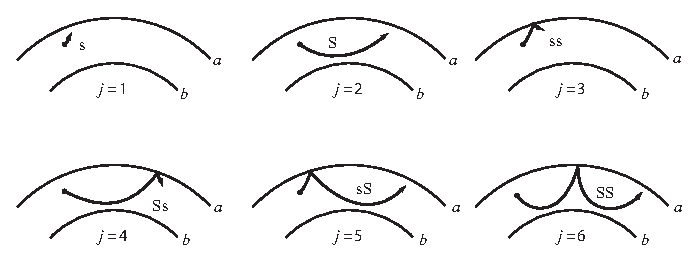
\includegraphics{../figures/chap12/fig23.eps}
\end{center}
\caption[Six S Paths]{\label{12.fig.Spaths}
区段II彩虹展开式~(\ref{12.Green6})中与$j=1\!-\!6$相应的直达、折返以及表面反射波的射线路径s, S, ss, Ss, sS和SS。这里假定震源({\em 点\/})位于接收点下方($r'<r$)。我们用s和ss表示没有折返的直达和表面反射波,Ss和sS表示表面反射并分别在第一和第二段路径上折返的波。这一命名方式对第12.1.1节中介绍的经典的射线命名规则做了少许(但合逻辑)的拓展。请与图~\ref{12.fig.ScSpaths}比较。
}
\end{figure}
\begin{figure}[!b]
\begin{center}
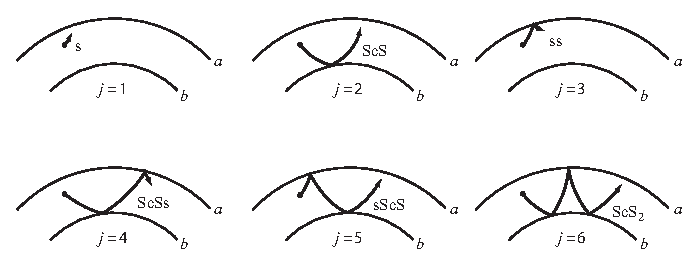
\includegraphics{../figures/chap12/fig24.eps}
\end{center}
\caption[Six ScS paths]{\label{12.fig.ScSpaths}
区段III彩虹展开式~(\ref{12.Green5})中与$j=1\!-\!6$相应的直达、表面反射波以及核幔边界反射的射线路径s, ScS, ss, ScSs, sScS和${\rm ScS}_2$。我们用s和ss表示没有折返的直达和表面反射波,ScSs和sScS表示先在核幔边界反射再在表面反射的波,反之亦然。这一命名方式仍然对第12.1.1节中介绍的经典的射线命名规则做了少许拓展。请与图~\ref{12.fig.Spaths}比较。
}
\end{figure}
我们可以确认公式~(\ref{12.tausubnu})和~(\ref{12.tausubnu2})中定义的$\tau_j$就是能够在震源和接收点半径$r'$ 和 $r$之间传播的各种波的截距时间,而$N_j$则是每一种波所折返的次数。图~\ref{12.fig.Spaths}显示了区段II中前六个射线路径s, S, ss, Ss, sS和SS。这里假定震源在接收点下方,即$r'<r$,因为这是观测地震学中通常的情形。图~\ref{12.fig.ScSpaths}中显示了对应的区段III中在核幔边界$r=b$处反射而不是折返的用“大写字母”表示的路径ScS, ScSs, sScS和${\rm ScS}_2$。在区段边界$p=b/\beta_{b+}$处折返指数$N_j$中的$\pi/2$不连续性是固定射线参数$p$的折返波的$\pi/2$焦散相移造成的。公式~(\ref{12.Green5})和~(\ref{12.Green6})中其它的量,尤其是比值$\tau/T$和震源至接收点截距时间$\tau_j$在跨越SH--${\rm ScS}_{\rm SH}$边界都是连续的。指数无穷求和项$\sum_{j=0}^{\infty}
\exp(-i\om\tau_j+iN_j\pi/2)$对于$\om>0$和下半平面的积分路径\mbox{$\Im{\rm m}\,p<0$}是收敛的,因为在实射线参数轴附近$\Im{\rm m}\,\tau_j\approx(\Im{\rm m}\,p)\Theta_j$,其中$\Theta_j$是与截距时间$\tau_j$相应的震源至接收点震中距。任何一个形如~(\ref{12.Green5})或~(\ref{12.Green6})的径向阶数求和到射线求和变换都被称为{\em 德拜\/} 或 {\em 彩虹展开\/},因为它们与彩虹理论得到的结果非常相似。
\index{Debye expansion}%
\index{rainbow expansion}%

将${\rm ScS}_{\rm SH}$和SH波的彩虹展开代入格林张量~(\ref{12.Green2}),我们发现因子$(1-C/c)^{-1}$被$\tau/T$抵消了。在$\om\rightarrow\infty$的极限下,行波的勒让德函数可以用其渐近展开式
\eq \label{12.Qasy}
Q_{\omega p-\subhalf}^{(1)}(\cos\Theta)\approx(2\pi\om p\sin\Theta)
^{-1/2}\exp(-i\om p\Theta+i\pi/4).
\en
\begin{figure}[!t]
\begin{center}
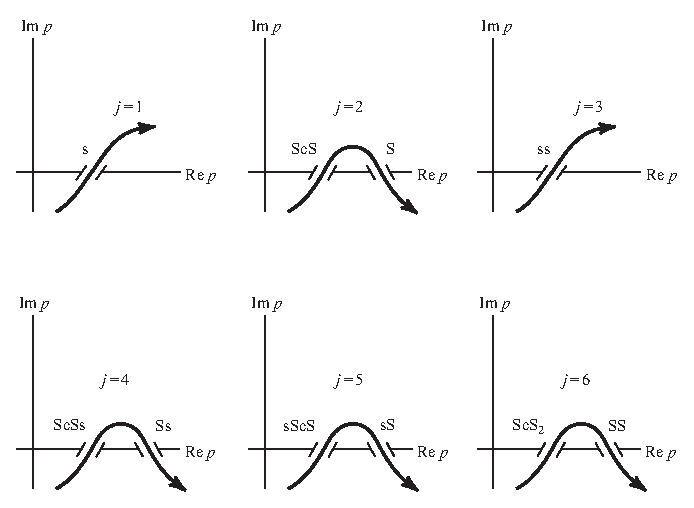
\includegraphics{../figures/chap12/fig25.eps}
\end{center}
\caption[Six Saddle Paths]{\label{12.fig.saddles}
复数射线参数平面示意图,显示叠加式~(\ref{12.Green7})中前六项的鞍点$p_k$的位置与取向。六幅图$j=1\!-\!6$的顺序({\em 从左上到右下\/})与图~\ref{12.fig.Spaths}图~\ref{12.fig.ScSpaths}中一样。每一幅图中,原来从$-\infty-i0$到$\infty-i0$的积分路径可以在鞍点处依照图中所示改变形状。
}
\end{figure}
近似到$\om^{-1}$的最低阶,$\brh\times\bdel_{\!1}$和 $\brh'\times\bdel_{\!1}^{\prime}$这两个算子仅仅需要作用在指数$\exp(-i\om p\Theta)$上,得到$(\brh\times\bdel_{\!1})(\brh'\times\bdel_{\!1}^{\prime})
\rightarrow\om^2p^2\bPhih\bPhihpr$, where $\bPhih=\bPhihpr$,
其中$\bPhih=\bPhihpr$是与射线平面垂直的单位矢量。最终的结果是高频SH波的格林张量可以写成
\eqa \label{12.Green7} \lefteqn{
\bG=\frac{1}{4\pi}\bPhih\bPhihpr
(rr'\beta\beta')^{-1}(2\pi\rho\rho'\sin\Theta)^{-1/2}} \nonumber \\
&&\mbox{}\times\int_{-\infty}^{\infty}
(q_{\beta}q_{\beta}^{\prime})
^{-1/2}\sum_{j=1}^{\infty}\exp[-i\om(\tau_j+p\Theta)] \nonumber \\
&&\mbox{}\qquad\qquad\times(\om p)^{1/2}\exp[i(N_j\pi/2-\pi/4)]\,dp.
\ena
公式~(\ref{12.Green7})中的下积分限$-\infty$在这里只具有象征意义,因为近似式~(\ref{12.Qasy})仅在$\Re{\rm e}\,p>0$时成立。
在使用该近似时我们已经预期到在$\om\rightarrow\infty$的极限下,$\bG$的主要贡献来自射线参数实轴正半部分的一个或多个{\em 鞍点\/}。
\index{saddle point}%

这些鞍点的位置$p_k$是由{\em 稳相条件\/}确定的
\eq \label{12.saddle}
\frac{d}{dp}(\tau_j+p\Theta)_{p=p_k}=0.
\en
由于$d\tau_j/dp=-\Theta_j$,条件~(\ref{12.saddle})简化为$\Theta_j(p_k)=\Theta$,因此鞍点正好落在与震源和接收点之间的SH波s、ScS、S、ss、ScSs、Ss、 sScS、sS、${\rm ScS}_2$、SS\hspace{0.3mm}\ldots相应的射线参数值上。图~\ref{12.fig.saddles}示意性地显示了前几个鞍点的形态。
\begin{figure}[!t]
\begin{center}
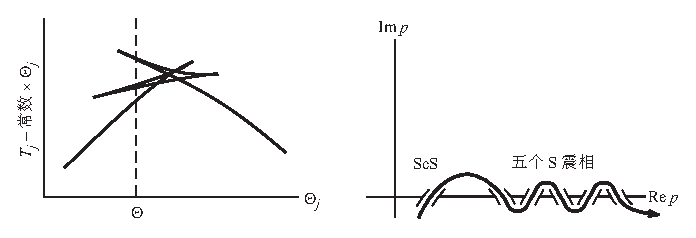
\includegraphics{../figures/chap12/fig26.eps}
\end{center}
\caption[More Saddles]{\label{12.fig.moresaddles}
({\em 左图\/})有两个上地幔中三重化的折返SH波的折合走时曲线。在震中距为$\Theta$的接收点处有五个SH波到达。({\em 右图\/})相应的公式~(\ref{12.Green7})中$j=2$项有五个鞍点(除ScS鞍点以外),其取向如图所示。
}
\end{figure}
如图所示,每一个鞍点由$(d^2\tau_j/dp^2)_{p=p_k}$的符号所确定的取向都有利于我们改变原来积分路径的形状以跨过鞍点。上地幔三重化震相带来额外的鞍点,如图~\ref{12.fig.moresaddles}所示。利用经典的鞍点近似(Lighthill \citeyear{lighthill78})对表达式~(\ref{12.Green7})中的每一项做计算,我们得到
\eqa \label{12.Green8} \lefteqn{
\bG=\frac{1}{4\pi}\bPhih\bPhihpr
(rr'\beta\beta')^{-1}(\rho\rho'\sin\Theta)^{-1/2}}
\nonumber \\
&&\mbox{}\times\sum_j\sum_k\left[p^{1/2}
(q_{\beta}q_{\beta}^{\prime})^{-1/2}
|d^2\tau_j/dp^2|^{-1/2}\right]_{p=p_k} \nonumber \\
&&\mbox{}\qquad\times
\exp(-i\om T_{jk}+iM_{jk}\pi/2),
\ena
其中$T_{jk}=\tau_j(p_k)+p_k\Theta$且
$M_{jk}=N_j-\half-\half
{\rm sgn}(d^2\tau_j/dp^2)_{p=p_k}$。
从物理上讲,公式~(\ref{12.Green8})中的双重求和是对所有震源$\bx'$和接收点$\bx$之间的几何SH射线路径。为简单起见,我们可以省略脚标$j$ 和 $k$,并利用几何扩散系数的表达式~(\ref{12.Rcoef}),将~(\ref{12.Green8})最终写成一个简洁的形式
\eq \label{12.GREEN}
\bG=\frac{1}{4\pi}\bPhih\bPhihpr
(\rho\rho'\beta\beta^{\prime 3})^{-1/2}
\sum_{\rm rays}\sR^{-1}\exp(-i\om T+iM\pi
\hspace{-0.2 mm}/2).
\en
公式~(\ref{12.GREEN})正好就是SH体波格林张量的经典的JWKB表达式(\v{C}erven\'{y}, Molotkov \&
P\v{s}en\v{c}\'{\i}k \citeyear{cerveny&al77};
\v{C}erven\'{y} \citeyear{cerveny85})。$T$是沿给定射线的走时,Maslov指数$M$是沿该射线传播的波所经过的焦散点的次数。因此,对于ScS$_{\rm SH}$波和下地幔折返的SH波,$M=0$;而对于${\rm SS}_{\rm SH}$波或者上地幔三重震相的\textcolor{red}{倒退分支}上的SH波,$M=1$。值得一提的是这种SH波因为经过焦散点而产生的非几何的$\pi/2$相位提前是在将$\bG_{\rm SH}(\bx,\bx';\om)$的表达式从模式叠加转换为射线叠加的过程中自然地出现的。

到此为止我们虽然仅仅关注了传播角距离$\Delta$小于$180^{\circ}$的$s=1$的情形,但是可以很容易地验证~(\ref{12.GREEN})的结果同样适用于公式~(\ref{eq:11.repre3})中$s=2,3,4,\ldots$的波。必要的话,的几何扩散因子~(\ref{12.Rcoef})中的$\sin\Theta$可以用$|\!\sin\Delta|$取代。对于这些绕地球多次的波,Maslov指数$M$同时追踪传播中经过震源及其对跖点所产生的“极点”相移。${\rm SS}_{\rm SH}$波的相移与其射线束面积的“反转”有关,因为有$d^2\tau_j/dp^2\rightarrow -d^2\tau_j/dp^2$的符号反转,而极点相移则与地理“反转”有关,因为$\sin\Delta\rightarrow-\sin\Delta$,也有一个符号反转,跟面波完全一样。
\index{Green tensor!SH|)}%
\index{tensor!SH Green|)}%

\subsection{P-SV 格林张量}
\index{Green tensor!P-SV|(}%
\index{tensor!P-SV Green|(}%

类似于~(\ref{12.Green2})的P-SV格林张量包含四项$\bG_1(\bx,\bx';\om)+\bG_2(\bx,\bx';\om)+
\bG_3(\bx,\bx';\om)+\bG_4(\bx,\bx';\om)$的叠加,分别为
\begin{displaymath}
\bG_1=\frac{\om^2}{2\pi}\,\brh\brh'\!
\int_{-\infty}^{\infty}\sum_{n=0}^{\infty}
\left(\frac{U_nU_n^{\prime}}{\om_n^2-\om^2}\right)
\!Q_{\omega p-\subhalf}^{(1)}
(\cos\Theta)\,(1\hspace{-0.3 mm}-\hspace{-0.3 mm}C/c)^{-1}\,p\,dp,
\end{displaymath}
\begin{displaymath}
\bG_2=\frac{\om}{2\pi}\,\brh\bdel_{\!1}^{\prime}\!
\int_{-\infty}^{\infty}\sum_{n=0}^{\infty}
\left(\frac{U_nV_n^{\prime}}{\om_n^2-\om^2}\right)
\!Q_{\omega p-\subhalf}^{(1)}
(\cos\Theta)\,(1\hspace{-0.3 mm}-\hspace{-0.3 mm}C/c)^{-1}\,dp,
\end{displaymath}
\begin{displaymath}
\bG_3=\frac{\om}{2\pi}\bdel_{\!1}\brh'\!
\int_{-\infty}^{\infty}\sum_{n=0}^{\infty}
\left(\frac{V_nU_n^{\prime}}{\om_n^2-\om^2}\right)
\!Q_{\omega p-\subhalf}^{(1)}
(\cos\Theta)\,(1\hspace{-0.3 mm}-\hspace{-0.3 mm}C/c)^{-1}\,dp,
\end{displaymath}
\begin{displaymath}
\bG_4=\frac{1}{2\pi}\bdel_{\!1}\bdel_{\!1}^{\prime}\!
\int_{-\infty}^{\infty}\sum_{n=0}^{\infty}
\left(\frac{V_nV_n^{\prime}}{\om_n^2-\om^2}\right)
\!Q_{\omega p-\subhalf}^{(1)}
(\cos\Theta)\,(1\hspace{-0.3 mm}-\hspace{-0.3 mm}C/c)^{-1}p^{-1}dp.
\end{displaymath}
\eq
\en
要得到完整的体波表达式$\bG_{\rm P\mbox{\scriptsize -}SV}(\bx,\bx';\om)$,我们需要在射线参数的每一个渐近区间中找到含有源点-接收点位移乘积$U_nU_n'$、$U_nV_n'$、$V_nU_n'$ 和 $V_nV_n'$的对径向阶数求和表达式的彩虹展开。没有一个与SH波中所使用的相当的简单傅里叶等式能够直接地把径向阶数求和转换为射线求和,尤其是在几个较高的区段,P-SV波的渐近本征频率与本征函数的解析表达式非常复杂。\textcite{zhao&dahlen96}展示了在区段III中如何得到所要的对复合地幔折返波的求和,在其它区段的相应的结果可以用类比的方法写出来。基本的构成要素是二项式展开,重复的应用可以得到所有可能的构成成分P, SV, K, I和${\rm J}_{\rm SV}$波的组合。一旦找到了所有的彩虹展开式,$\bG_1$到$\bG_4$在$\om\rightarrow\infty$极限下对射线参数$p$的积分就可以像前面的做法一样,通过在正实轴上的鞍点处改变积分路径的形状计算得到。用这种方法最终得到的P-SV波格林张量的表达式可以写成
\eq \label{12.PGREEN}
\bG=\frac{1}{4\pi}\sum_{\rm rays}
\betah\betah^{\raise-.1ex\hbox{$\scriptstyle\prime$}}
(\rho\rho'vv^{\prime 3})^{-1/2}\hspace{0.2 mm}
\Pi\hspace{0.2 mm}\sR^{-1}\exp(-i\om T+iM\pi
\hspace{-0.2 mm}/2),
\en
其中的求和是对震源$\bx'$和接收点$\bx$之间的所有可能的射线。与前面一样,$T$是射线路径上所有波的总走时,$\sR$是相应的几何扩散系数,$M$是Maslov指数,追踪径向与水平向所经过的焦散点的次数。速度$v^{\prime}$ 和
$v$分别是射线上离开震源一段和到达接收点一段的波速,而$\betah^{\raise-.1ex\hbox{$\scriptstyle\prime$}}$ 和
$\betah$则是~(\ref{12.polar})中的相应的偏振矢量。SH波表达式~(\ref{12.GREEN})中没有的新的因子$\Pi$在传播路径上所遇到的各个不连续面处所有(能量$)^{1/2}$反射和透射系数的乘积,例如,对于ScP转换波,$\Pi=\grave{\sS}\hspace{-0.1 mm}\acute{\sP}$,而对于穿过地心的PKIKP波,$\Pi=\grave{\sP}\hspace{-0.3 mm}
\grave{\sK}\,\grave{\sK}\grave{\sI}\hspace{0.6 mm}
\acute{\sI}\hspace{-0.1 mm}\acute{\sK}\,
\acute{\sK}\hspace{-0.2 mm}\acute{\sP}$。

我们也可以把~(\ref{12.PGREEN})看作是JWKB体波格林张量$\bG_{\rm SH}+\bG_{\rm P\mbox{\scriptsize -}SV}$的普遍公式,
只需要让求和指数把SH波和P-SV波都包括进来。无论水平传播方向如何,SH波的质点运动方向总是在横向,
\index{particle motion!SH}%
\index{polarization!SH}%
即$\betah\betah'=\bPhih\bPhihpr$,而且串接的(能量$)^{1/2}$的系数都是$\Pi=1$。正如预期的,对于固定的震源位置$\bx'$,沿任一射线上$\bG(\bx,\bx';\om)$对接收点位置$\bx$的依赖性与几何振幅变化定律~(\ref{12.amprule3})一致。值得注意的是,JWKB格林张量满足动力学的震源-接收点互易原理
\index{reciprocity!body waves}%
\eq
\bG(\bx,\bx';\om)=\bG^{\rm T}(\bx',\bx;\om),
\en
因为反射-透射系数~(\ref{12.scatsym})、几何扩散 (\ref{12.Rcoef2})、
和Maslov指数~(\ref{12.Maslovsymm})都是对称的。如果将震源与接收点的位置交换,即$\bx\rightarrow\bx'$ 和 $\bx'\rightarrow\bx$,震源与接收点的偏振矢量交换并反向,即$\betah\rightarrow -\betah^{\raise-.1ex\hbox{$\scriptstyle\prime$}}$
和 $\betah^{\raise-.1ex\hbox{$\scriptstyle\prime$}}\rightarrow -\betah$,那么沿给定射线传播的能量将按原路返回。在反转的射线上,所有在界面反射与透射时的转换均以相反的方式发生。例如,ScP波的互易之后变为ScP反之亦然。
\index{Green tensor!P-SV|)}%
\index{tensor!P-SV Green|)}%

\renewcommand{\thesubsection}{$\!\!\!\raise1.3ex\hbox{$\star$}\!\!$
\arabic{chapter}.\arabic{section}.\arabic{subsection}}
\subsection{希尔伯特变换公式汇编}
\index{Hilbert transform|(}%
\renewcommand{\thesubsection}{\arabic{chapter}.
\arabic{section}.\arabic{subsection}}

要计算~(\ref{12.PGREEN})中的JWKB格林张量的傅里叶反变换,并将得到的时间域结果推广到在焦散点附近也成立,我们需要另外一些数学符号,将在本节来介绍。所有在本节介绍的关系要么是众所周知,要么证明很容易,因此我们在此不做任何证明。如果对这些内容的系统性讨论有兴趣的话,可以参考\textcite{bracewell65}。

一个实的时间域信号$f(t)$的{\em 希尔伯特变换\/}的定义为
\index{Hilbert transform}%
\eq \label{12.hilbert}
f_{\rm H}(t)=\sH f(t)=\frac{1}{\pi}\pvint_{\!\!-\infty}^{\,\,\infty}
\frac{f(t')}{t'-t}dt'.
\en
通过希尔伯特反变换,我们可以把$f(t)$用$f_{\rm H}(t)$来表示
\eq \label{12.hilbert2}
f(t)=\sH^{-1}f_{\rm H}(t)=-\frac{1}{\pi}\pvint_{\!\!-\infty}^{\,\,\infty}
\frac{f_{\rm H}(t')}{t'-t}dt'.
\en
(\ref{12.hilbert})--(\ref{12.hilbert2})中带一横线的积分表示柯西主值,如公式~(\ref{6.PVdef}),是通过切除了$(t'-t)^{-1}$的奇异性定义的。$M$次连续的希尔伯特变换可以表示为
\eq \label{12.hilbert3}
f_{\rm H}^{(M)}(t)=\underbrace{\sH\cdots\sH}_{M\,\rm times}f(t).
\en
It is noteworthy that $f_{\rm H}^{(0)}(t)=f(t)$,
$f_{\rm H}^{(1)}(t)=f_{\rm H}(t)$ and $f_{\rm H}^{(2)}(t)=-f(t)$.
值得指出的是$f_{\rm H}^{(0)}(t)=f(t)$,
$f_{\rm H}^{(1)}(t)=f_{\rm H}(t)$以及 $f_{\rm H}^{(2)}(t)=-f(t)$。

对应于$f(t)$的复数{\em 解析信号\/}的定义为
\index{analytic signal}%
\eq \label{12.anasignal}
F(t)=f(t)-if_{\rm H}(t).
\en
(\ref{12.anasignal})的希尔伯特变换是$F_{\rm H}(t)=f_{\rm H}(t)+if(t)$。希尔伯特变换将一个信号的每一个傅里叶分量的相位提前$\pi/2$。因此,如果$f(\om)$是$f(t)$的傅里叶变换,那$f(\om)\exp(iM\pi/\hspace{-0.2 mm}2)$就是$f_{\rm H}^{(M)}(t)$的傅里叶变换,即
\eq \label{12.hilbert4}
f_{\rm H}^{(M)}(t)=\frac{1}{\pi}\,\Re{\rm e}\!\int_0^{\infty}
f(\om)\exp i(\om t+M\pi/\hspace{-0.2 mm}2)\,d\om.
\en
特别地,狄拉克函数的多重希尔伯特变换是
\eq \label{12.hilbert5}
\delta_{\rm H}^{(M)}(t)=\frac{1}{\pi}\,\Re{\rm e}\!\int_0^{\infty}
\exp i(\om t+M\pi/\hspace{-0.2 mm}2)\,d\om.
\en
上式的前三个例子是
\eq \label{12.deltaH}
\delta_{\rm H}^{(0)}(t)
=\delta(t),\qquad\delta_{\rm H}^{(1)}(t)=-(\pi t)^{-1},\qquad
\delta_{\rm H}^{(2)}(t)=-\delta(t).
\en
{\em 解析狄拉克函数\/}为
\index{analytic delta function}%
\index{delta function!analytic}%
$\Delta(t)=\delta(t)-i\delta_{\rm H}(t)
=\delta(t)+i(\pi t)^{-1}$。

两个时间域信号$f(t)$
和 $g(t)$之间的{\em 卷积\/}当然是
\index{convolution}%
\eq \label{12.convol}
f(t)*g(t)=\int_{-\infty}^{\infty}f(t')g(t-t')dt'.
\en
时间域中的卷积相当于频率域中的相乘,也就是说,$f(t)*g(t)$的傅里叶变换是$f(\om)g(\om)$。希尔伯特变换~(\ref{12.hilbert})及其反变换~(\ref{12.hilbert2})可以写成正规的卷积形式: $f_{\rm H}(t)=-f(t)*(\pi t)^{-1}$
and $f(t)=f_{\rm H}(t)*(\pi t)^{-1}$。卷积是互易的: $f(t)*g(t)=g(t)*f(t)$。时间微分(用函数符号上面一点表示)和希尔伯特变换可以从卷积中的一个信号转移到另一个:$f(t)*\dot{g}(t)=\dot{f}(t)*g(t)$和
$f(t)*g_{\rm H}(t)=f_{\rm H}(t)*g(t)$。两个希尔伯特变换的卷积是$f_{\rm H}(t)*g_{\rm H}(t)=-f(t)*g(t)$。一个时间延迟的信号$f(t-T)$的傅里叶变换是$f(\om)\exp(-i\om T)$。在卷积中,哪个信号被时间延迟了是无关紧要的:$f(t)*g(t-T)=f(t-T)*g(t)$。如果$f(t)$ 和 $g(t)$的解析信号分别为$F(t)$ 和 $G(t)$,则$f(t)*\Re{\rm e}\,[G(t)]=\Re{\rm e}\,[F(t)]*g(t)$。一个与频率无关的复常数$\sC=\sA+i\sB$的傅里叶反变换为$\Re{\rm e}\,[\sC\Delta(t)]
=\sA\delta(t)+\sB\delta_{\rm H}(t)$。更普遍地,该常数与$f(\om)$相乘的傅里叶反变换为$\Re{\rm e}\,[\sC F(t)]=\sA f(t)+\sB f_{\rm H}(t)$。

在我们的讨论中比较有用的两个希尔伯特变换对是
\eq \label{12.chapman}
\upsilon(t)=\frac{1}{\pi}\,\Re{\rm e}\!\int_0^{\infty}
\om^{-1/2}\exp i(\om t-\pi\hspace{-0.2 mm}/\hspace{-0.2 mm}4)\,d\om=
\frac{H(t)}{\sqrt{\pi t}},
\en
\eq \label{12.chapman2}
\upsilon_{\rm H}(t)=\frac{1}{\pi}\,\Re{\rm e}\!\int_0^{\infty}
\om^{-1/2}\exp i(\om t+\pi\hspace{-0.2 mm}/\hspace{-0.2 mm}4)\,d\om=
\frac{H(-t)}{\sqrt{-\pi t}}
\en
和
\eq \label{12.chapman3}
\lambda(t)=\frac{1}{\pi}\,\Re{\rm e}\!\int_0^{\infty}
\om^{1/2}\exp i(\om t-\pi\hspace{-0.2 mm}/\hspace{-0.2 mm}4)\,d\om=
-\frac{d}{dt}\frac{H(-t)}{\sqrt{-\pi t}},
\en
\eq \label{12.chapman4}
\lambda_{\rm H}(t)=\frac{1}{\pi}\,\Re{\rm e}\!\int_0^{\infty}
\om^{1/2}\exp i(\om t+\pi\hspace{-0.2 mm}/\hspace{-0.2 mm}4)\,d\om=
\frac{d}{dt}\frac{H(t)}{\sqrt{\pi t}},
\en
其中$H(t)$为阶梯函数。很明显,我们有
$\lambda(t)=-\dot{\upsilon}_{\rm H}(t)$
和 $\lambda_{\rm H}(t)=\dot{\upsilon}(t)$。
相关的卷积关系有
\eq \label{12.chapman5}
\upsilon(t)*\upsilon(t-T)=-\upsilon_{\rm H}(t)*\upsilon_{\rm H}(t-T)
=H(t-T),
\en
\eq
\label{12.chapman6}
\lambda(t)*\upsilon_{\rm H}(t-T)=-\lambda_{\rm H}(t)*\upsilon(t-T)
=\delta(t-T),
\en
\eq
\label{12.chapman7}
\lambda(t)*\upsilon(t-T)=-\lambda_{\rm H}(t)*\upsilon_{\rm H}(t-T)
=-\delta_{\rm H}(t-T),
\en
\eq
\label{12.chapman8}
\lambda(t)*\lambda(t-T)=-\lambda_{\rm H}(t)*\lambda_{\rm H}(t-T)
=-\dot{\delta}(t-T).
\en
值得注意的是~(\ref{12.chapman})--(\ref{12.chapman4})中的信号的单边特性。相反,解析的复信号$\Lambda(t)=\lambda(t)-i\lambda_{\rm H}(t)$
和 $\Upsilon(t)=\upsilon(t)-i\upsilon_{\rm H}(t)$都是双边的。
\index{Hilbert transform|)}%

\renewcommand{\thesubsection}{$\!\!\!\raise1.3ex\hbox{$\star$}\!\!$
\arabic{chapter}.\arabic{section}.\arabic{subsection}}
\subsection{时间域格林张量}
\index{tensor!Green!time-domain|(}%
\index{Green tensor!time-domain|(}%
\renewcommand{\thesubsection}{\arabic{chapter}.
\arabic{section}.\arabic{subsection}}

从公式~(\ref{12.PGREEN})的傅里叶逆变换得到的射线理论的格林张量$\bG(\bx,\bx';t)$为
\eq \label{12.timeGreen}
\bG=\frac{1}{4\pi}\sum_{\rm rays}
\betah\betah^{\raise-.1ex\hbox{$\scriptstyle\prime$}}
(\rho\rho'vv^{\prime 3})^{-1/2}\hspace{0.2 mm}
\Pi\hspace{0.2 mm}\sR^{-1}\delta_{\rm H}^{(M)}(t-T),
\en
其中$\delta_{\rm H}^{(M)}(t)$在~(\ref{12.hilbert5})中给定, 同时我们也假定所有在乘积$\Pi$中串在一起的反射和透射系数都是实的。所有$M=0$的体波都沿最短走时路径传播,且表现因果的$\delta(t-T)$时间依赖性,
\index{causality}%
而$M=1$的波则沿极小极大走时路径传播,且有非因果的$\delta_{\rm H}(t-T)=-[\pi(t-T)]^{-1}$时间依赖性。这一希尔伯特变换导致了人们熟知的PP, SS以及其它经过多次反射和折射后经过焦散点的震相的突然启动的特征(Choy \& Richards \citeyear{choy&richards75})。

在焦散点非常邻近的地方,由于几何扩散因子的倒数$\sR^{-1}$ 的发散性,射线理论{\em 本身\/}不再成立。但是,很容易将~(\ref{12.timeGreen})的结果进行推广使其处处规则,包括在焦散点附近。为简单起见,我们还是将关注点集中在传播距离小于地球半圈的$s=1$的波。回到SH波的格林张量$\bG_{\rm SH}(\bx,\bx';\om)$的积分表达式~(\ref{12.Green7}),我们注意到唯一的频率依赖性是显式的$\om^{1/2}\exp[-i\om(\tau_j+p\Theta)]$。因此,$\bG_{\rm SH}(\bx,\bx';t)$的傅里叶反变换可以{\em 精确地\/}计算。将指数上依赖于$p$的量表示成
\eq \label{12.Gammadef}
\Gamma_j(p)=\tau_j(p)+p\hspace{0.2 mm}\Theta
=T_j(p)+p[\Theta-\Theta_j(p)],
\en
我们得到一个无穷项的卷积求和:
\eqa \label{12.timeGreen2} \lefteqn{
\bG=\frac{1}{4\pi}\bPhih\bPhihpr
(rr'\beta\beta')^{-1}(2\rho\rho'\sin\Theta)^{-1/2}} \nonumber \\
&&\mbox{}\qquad\qquad\times
\sum_{j=1}^{\infty}\lambda_{\rm H}^{(N_j)}(t)*\sigma_j(t),
\ena
其中
\eq \label{12.timeGreen3}
\lambda_{\rm H}^{(N_j)}(t)=\frac{1}{\pi}\,\Re{\rm e}\!\int_0^{\infty}
\om^{1/2}\exp i(\om t+N_j\pi/\hspace{-0.2 mm}2
-\pi\hspace{-0.2 mm}/\hspace{-0.2 mm}4)\,d\om,
\en
\eq \label{12.timeGreen4}
\sigma_j(t)=\int_{-\infty}^{\infty}p^{1/2}(\pi q_{\beta}
q_{\beta}^{\prime})^{-1/2}\,\delta(t-\Gamma_j)\,dp.
\en
每一项卷积的前一个函数是单边信号~(\ref{12.chapman3})的$N_j$次希尔伯特变换。公式~(\ref{12.timeGreen4})中的积分可以用狄拉克函数的\textcolor{red}{复制性质}来计算:
\eqa \label{12.timeGreen5} \lefteqn{
\sigma_j(t)=\sum_{t=\Gamma_j}p^{1/2}(\pi q_{\beta}
q_{\beta}^{\prime})^{-1/2}|d\hspace{0.2 mm}\Gamma_j/dp|^{-1}} \nonumber \\
&&\hspace{1.6 mm}=\sum_{t=\Gamma_j}p^{1/2}(\pi q_{\beta}
q_{\beta}^{\prime})^{-1/2}|\Theta-\Theta_j|^{-1},
\ena
这里第二个等式是由于
$d\hspace{0.2 mm}\Gamma_j/dp=-\Theta_j$。
(\ref{12.timeGreen5})中的求和是对所有满足方程$t=\Gamma_j(p)$的射线参数$p$,如图~\ref{12.fig.chapman}所示。
\begin{figure}[!t]
\begin{center}
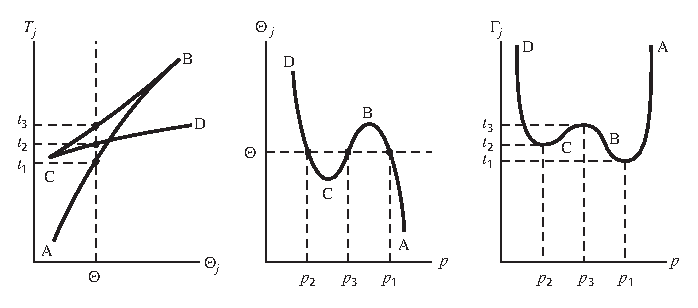
\includegraphics{../figures/chap12/fig27.eps}
\end{center}
\caption[AkiRichardsFig9.21]{\label{12.fig.chapman}
计算函数$\sigma_j(t)$的示意图。({\em 左图\/})$T_j(p)$ 与 $\Theta_j(p)$之间的三重化走时曲线,在B和C点发生焦散。震中距固定为$\Theta$的接收点有三个几何震相在$t_1,t_2,t_3$时刻到达。({\em 中图\/})相应的射线参数$p_1,p_2,p_3$满足$\Theta_j(p_k)=\Theta$。({\em 右图\/})当$t<t_1$时,没有$t=\Gamma_j(p)$的交点;当$t_1<t<t_2$时,有两个交点;当$t_2<t<t_3$时,有四个交点。焦散点B和C在$\Theta_j(p)$上表现为极值点,而在$\Gamma_j(p)$上表现为拐点。相位函数的斜率$d\hspace{0.1 ex}\Gamma_j/dp=\Theta-\Theta_j$在$p_1,p_2,p_3$处为零,因而$\sigma_j(t)$在射线理论到时$t_1,t_2,t_3$时为零。请注意,如果$t_1<t_2<t_3$,则$p_2<p_3<p_1$。
}
\end{figure}
$|\Theta-\Theta_j|^{-1}$在射线理论到时$T_{jk}=\tau_j(p_k)+p_k\Theta$时的奇异性可以通过将$\sigma_j(t)$在数值化间隔上做平均来得到抑制(Dey-Sarkar \& Chapman \citeyear{dey-sarkar&chapman78};
Chapman, Chu \& Lyness \citeyear{chapman&al88})。

将$\Gamma_j(p)$在其极值$p_k$附近用抛物线近似:
\eq
\Gamma_j(p)=T_{jk}+\half(d^2\tau_j/dp^2)_{p=p_k}
(p-p_k)^2.
\en
我们可以从形式上重建射线理论的结果。在此近似下,交点$t=\Gamma_j(p)$出现在对称分布的点上
\eq \label{12.inters}
p=p_k\pm \left|\frac{2(t-T_{jk})}
{(d^2\tau_j/dp^2)_{p=p_k}}\right|^{1/2}.
\en
将~(\ref{12.inters})代入公式~(\ref{12.timeGreen5}),我们得到
\eqa \label{12.sigmappr} \lefteqn{
\sigma_j(t)=\sum_k\left[p^{1/2}
(q_{\beta}q_{\beta}^{\prime})^{-1/2}
|d^2\tau_j/dp^2|^{-1/2}\right]_{p=p_k}} \nonumber \\
&&\mbox{}\times\left\{\begin{array}{ll}
\sqrt{2}\,\upsilon(t-T_{jk}) &
\mbox{if ${\rm sgn}(d^2\tau_j/dp^2)_{p=p_k}>0$} \\
\vspace{-1.5 mm} & \vspace{-1.5 mm} \\
\sqrt{2}\,\upsilon_{\rm H}(t-T_{jk}) &
\mbox{if ${\rm sgn}(d^2\tau_j/dp^2)_{p=p_k}<0$.}
\end{array}\right.
\ena
应用等式
\eq
\lambda_{\rm H}^{(N_j)}(t)*\upsilon(t-T_{jk})=
-\delta_{\rm H}^{(N_j+1)}(t-T_{jk}),
\en
\eq
\lambda_{\rm H}^{(N_j)}(t)*\upsilon_{\rm H}(t-T_{jk})=
\delta_{\rm H}^{(N_j)}(t-T_{jk}),
\en
我们发现~(\ref{12.timeGreen2})可以转化为~(\ref{12.Green8})的双重求和的时间域形式:
\eqa \label{12.tGreen8} \lefteqn{
\bG=\frac{1}{4\pi}\bPhih\bPhihpr
(rr'\beta\beta')^{-1}(\rho\rho'\sin\Theta)^{-1/2}}
\nonumber \\
&&\mbox{}\times\sum_j\sum_k\left[p^{1/2}
(q_{\beta}q_{\beta}^{\prime})^{-1/2}
|d^2\tau_j/dp^2|^{-1/2}\right]_{p=p_k} \nonumber \\
&&\mbox{}\qquad\times
\delta_{\rm H}^{(M_{jk})}(t-T_{jk}).
\ena
${\rm SS}_{\rm SH}$与其它$M=1$的极小极大走时震相的希尔伯特变换$\delta_{\rm H}(t-T_{jk})=-[\pi(t-T_{jk})]^{-1}$再次自动地产生。当图~\ref{12.fig.chapman}中$\Gamma_j(p)$的相邻极值点如$p_2,p_3$ 或 $p_3,p_1$考得过近而互相之间或与中间的焦散点B或C发生“干涉”时,(\ref{12.inters})中的二次近似会变得不够精确。然而,表达式~(\ref{12.timeGreen2})是一致有效的,无论接收点是否靠近焦散点。甚至重叠的三重化震相和邻近的多个焦散点都能自动处理。此外,计算一致成立的表达式~(\ref{12.timeGreen2})所需的数值工作也只比计算~(\ref{12.tGreen8})中的JWKB结果稍微多一点点。

对公式~(\ref{12.timeGreen5})中交点$t=\Gamma_j(p)$的搜索是在整个SH波的射线参数范围$0< p< a/\beta_a$,因此,$\sigma_2(t)$包含了相当于${\rm ScS}_{\rm SH}$和折返SH波的震相,甚至可能还有三重震相。在实际中,这种做法很少采用。相反,地震学中“清楚的”震相如${\rm ScS}_{\rm SH}$和远离液态外核影区的三重震相是单独合成的。采用这一不同的观点,我们将方程~(\ref{12.timeGreen2})用通用的符号写为:
\eqa \label{12.timeGreen6} \lefteqn{
\bG=\frac{1}{4\pi}\bPhih\bPhihpr
(rr'\beta\beta')^{-1}(2\rho\rho'\sin\Theta)^{-1/2}} \nonumber \\
&&\mbox{}\qquad\qquad\times
\sum_{\rm rays}\lambda_{\rm H}^{(N)}(t)*\sigma(t),
\ena
其中$N$是沿射线不同的折返射线个数,而且每一个SH波都算是一个“射线”,即使是三重震相。表达式~(\ref{12.timeGreen6})可以很容易地推广到P-SV波,只要考虑到偏振方向以及震源和接收点处波速的变化,还有因与界面相互作用需要的一连串反射与透射系数$\Pi$。包括所有$s=1$的波的完整的时间域格林张量$\bG_{\rm SH}+\bG_{\rm P\mbox{\scriptsize -}SV}$可以写成
\eqa \label{12.timeGreen7} \lefteqn{
\bG=\frac{1}{4\pi}\sum_{\rm rays}
\betah\betah^{\raise-.1ex\hbox{$\scriptstyle\prime$}}
(rr'vv')^{-1}(2\rho\rho'\sin\Theta)^{-1/2}} \nonumber \\
&&\mbox{}\qquad\qquad\times
\Re{\rm e}\,[\Lambda_{\rm H}^{(N)}(t)*\sigma(t)],
\ena
其中
\eq \label{12.LambdaH}
\Lambda_{\rm H}^{(N)}(t)=\underbrace{\sH\cdots\sH}_{N\,\rm times}
\Lambda(t)=\lambda_{\rm H}^{(N)}(t)-i\lambda_{\rm H}^{(N+1)}(t),
\en
\eq \label{12.timeGreen8}
\sigma(t)=\sum_{t=\Gamma}p^{1/2}(\pi qq')^{-1/2}
\Pi\,|d\hspace{0.2 mm}\Gamma/dp|^{-1}.
\en
只要$\Im{\rm m}\,\Pi=0$,$\Re{\rm e}\,[\Lambda(t)_{\rm H}^{(N)}*\sigma(t)]$就会如在~(\ref{12.timeGreen6})中一样退化为$\lambda(t)_{\rm H}^{(N)}*\sigma(t)$。(\ref{12.timeGreen7})是一个更一般的形式,它包含解析信号$\Lambda(t)=\lambda(t)-i\lambda_{\rm H}(t)$的$N$次希尔伯特变换,同时适用于过临界($\Pi$为复数)与亚临界($\Pi$为实数)震相。

第一个形如(12.256)的一致有效的射线叠加结果是Chapman (\citeyear{chapman76};
\citeyear{chapman78})得到的。他建议将这一表达式称为“WKBJ地震图”以确认其直接来源于径向JWKB近似这一事实。事实上,作为一个能够将任何JWKB结果拓展到适用于焦散点附近的通用技术,(\ref{12.timeGreen7})的实现方法是不寻常的(Maslov 1972; Maslov & Fedoriuk 1981; Chapman & Drummond 1982; Liu & Tromp 1996)。我们更倾向于用简称JWKB来代表严格的射线理论结果~(\ref{12.timeGreen}),而把一致有效的表达式(\ref{12.timeGreen7})称为{\em Chapman-Maslov格林张量\/}。
\index{tensor!Green!Chapman-Maslov}%
\index{Green tensor!Chapman-Maslov}%
\index{tensor!Green!time-domain|)}%
\index{Green tensor!time-domain|)}%

\renewcommand{\thesubsection}{$\!\!\!\raise1.3ex\hbox{$\star$}\!\!$
\arabic{chapter}.\arabic{section}.\arabic{subsection}}
\subsection{JWKB 和 Chapman-Maslov 地震图}
\label{12.sec.JWKB-Chap}
\index{seismogram!JWKB|(}%
\index{JWKB seismogram|(}%
\index{seismogram!Chapman-Maslov|(}%
\index{Chapman-Maslov seismogram|(}%
\renewcommand{\thesubsection}{\arabic{chapter}.
\arabic{section}.\arabic{subsection}}

最后,我们考虑一个震源位于$\bx_{\rm s}$的地震点源的高频体波响应。我们允许有限时长的破裂,假定震源是同步的,具有如下形式的依赖频率的矩张量
\eq
\bM(\om)=\sqrt{2}M_0\hat{\bM}_{\,}m(\om).
\en
如第5.4.5节所述,$M_0$和$\hat{\bM}$ 分别为标量地震矩和单位机制张量,$m(\om)$为归一化震源时间函数$\dot{m}(t)$的傅里叶变换。精确的频率域位移响应可以用格林张量表示为
\eq
\bs(\bx,\om)=(i\om)^{-1}\bM(\om)\!:\!\bdel_{\!{\rm s}}
\bG^{\rm T}(\bx,\bx_{\rm s};\om).
\en
精确到$\om^{-1}$的一阶项,对震源坐标的梯度$\bdel_{\!{\rm s}}$ 仅需要作用于JWKB表达式~(\ref{12.PGREEN})中快速振荡的$\exp(-i\om T)$因子上,得到一个乘子$\bdel_{\!{\rm s}}\rightarrow
i\om v_{\rm s}^{-1}\bph_{\rm s}$,其中$\bph_{\rm s}$ 是出发时的单位慢度矢量。将接收点和震源相关的因子分别统一表示成
\eq \label{12.RECVR}
\Xi=(\rho v)^{-1/2}(\bnuh\cdot\betah),
\en
\eq \label{12.SOURC}
\Sigma=\sqrt{2}M_0(\rho_{\rm s}v_{\rm s}^5)^{-1/2}
[\hat{\bM}\!:\!\half(\bph_{\rm s}\betah_{\rm s}
+\betah_{\rm s}\bph_{\rm s})],
\en
我们可以将标量位移$s(\om)=\bnuh\cdot\bs(\bx,\om)$表示为
\eq \label{12.DISP}
s(\om)=\frac{1}{4\pi}\sum_{\rm rays}\Xi\hspace{0.4 mm}\Sigma
\hspace{0.4 mm}\Pi\hspace{0.4 mm}\sR^{-1}
m(\om)\exp(-i\om T+iM\pi/\hspace{-0.2 mm}2).
\en
方程~(\ref{12.DISP})的傅里叶反变换得到的时间域响应是
\eq \label{12.DISP2}
s(t)=\frac{1}{4\pi}\sum_{\rm rays}\Xi\hspace{0.4 mm}\Sigma
\hspace{0.4 mm}\Pi\hspace{0.4 mm}\sR^{-1}
\dot{m}_{\rm H}^{(M)}(t-T).
\en
所有最短走时震相如P和S波的{\em 脉冲形状\/}都是$\dot{m}(t)$,
\index{pulse shape}%
而每一次经过焦散点都会对这一远场震源时间函数做一次希尔伯特变换。       $\hat{\bM}\!:\!\half(\bph_{\rm s}\betah_{\rm s}
+\betah_{\rm s}\bph_{\rm s})$这个量是出射波在包围震源的震源球上的{\em 辐射花样\/}。
\index{radiation pattern!body-wave}%
\index{body-wave radiation pattern}%
特别要注意的是,P波的振幅与$\bph_{\rm s}\cdot\hat{\bM}\cdot\bph_{\rm s}$成正比,与我们在第5.4.4节中关于沙滩球的讨论一致。

非弹性衰减及相应的频散可以通过引入复数波速来处理:
\eq
v=v_0[1+\half iQ^{-1}+\invpi Q^{-1}\ln
(\om\hspace{-0.2 mm}/\hspace{-0.2 mm}\om_0)],
\en
其中$v_0$是在频率为$\om_0$时的参考波速,可能是$\alpha_0$ 或 $\beta_0$,$Q$可能是$Q_{\alpha}$ 或 $Q_{\beta}$。我们忽略非弹性对射线几何的影响,但在计算走时中对频率域的射线求和~(\ref{12.DISP})做如下替换来包含其影响:
\eq \label{12.Tpert}
T\rightarrow T-\half iT^{\ast}-\invpi T^{\ast}\ln
(\om\hspace{-0.2 mm}/\hspace{-0.2 mm}\om_0).
\en
(\ref{12.Tpert})中与频率无关的{\em 衰减时间\/}$T^{\ast}$为
\index{attenuation time}%
\index{T@$T^{\ast}$}%
\eq \label{12.Tstar}
T^{\ast}=\int_{\subx^{\prime}}^{\subx}\frac{ds}{v_0Q}
=\int_{\subx^{\prime}}^{\subx}\frac{v_0^{-2}}{q_0Q}\,dr,
\en
其中$q_0=(v_0^{-2}-p^2r^{-2})^{1/2}$,且积分是沿组成射线的所有部分。
典型的数值是对远震P波$T^{\ast}\approx 1\!-\!2$秒,对远震S波$T^{\ast}\approx 4\!-\!8$秒。在时间域,衰减和频散可以用一个额外的卷积来纳入,JWKB响应~(\ref{12.DISP2})成为
\eq \label{12.DISP3}
s(t)=\frac{1}{4\pi}\sum_{\rm rays}\Xi\hspace{0.4 mm}\Sigma
\hspace{0.4 mm}\Pi\hspace{0.4 mm}\sR^{-1}
\dot{m}_{\rm H}^{(M)}(t-T)*a(t),
\en
其中
\eq \label{12.atten}
a(t)=\frac{1}{\pi}\,\Re{\rm e}\int_0^{\infty}
\exp i\om\!\left[t+\half iT^{\ast}+\invpi T^{\ast}\ln
(\om\hspace{-0.2 mm}/\hspace{-0.2 mm}\om_0)\right]d\om.
\en
由于公式~(\ref{12.atten})中的因子$\exp(-\half\om T^{\ast})$,高频波的衰减远比低频波要快。这会导致$M=0$的弹性脉冲$\dot{m}(t-T)$ 的展宽与阻尼效应。非弹性频散会使脉冲有所延迟,其大小不仅依赖于$T^{\ast}$,也依赖于短吸收带周期一侧$\tau_{\rm m}$的位置(Minster \citeyear{minster78}; \citeyear{minster80})。

\begin{figure}[!t]
\begin{center}
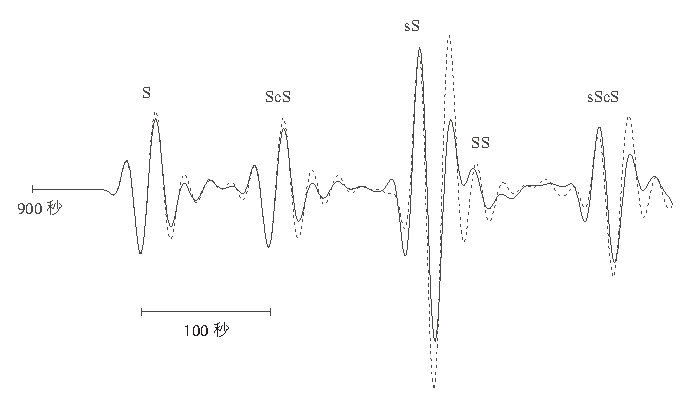
\includegraphics{../figures/chap12/fig28.eps}
\end{center}
\caption[RaysvsModes]{\label{12.fig.jeroen}
射线理论结果~(\ref{12.DISP3})与精确的PREM模式叠加结果~(\ref{10.DISPUGLY})的比较。震源是1994年6月9日的玻利维亚深震,震源时间函数为狄拉克函数即瞬时脉冲:$\dot{m}(t)=\delta(t)$。射线理论({\em 实线\/})和精确({\em 点线\/})结果显示的都是在密苏里州Cathedral Cave的台站CCM的地面加速度$a(t)=\ddot{s}(t)$的横向分量。为突出体波震相,两个加速度图都做了相同的$20\!-\!80$秒的带通滤波。在射线叠加中仅包括了标识的SH、${\rm ScS}_{\rm SH}$、
${\rm sS}_{\rm SH}$, ${\rm SS}_{\rm SH}$ 和
${\rm sScS}_{\rm SH}$震相。
}
\end{figure}
(\ref{12.DISP3})可以很容易地推广到也适用于焦散点附近的形式:
\eqa \label{12.DISP4} \lefteqn{
s(t)=\frac{1}{4\pi}\sum_{\rm rays}\,
[r^{-1}(2v\sin\Theta)^{-1/2}\Xi\,]
[r_{\rm s}^{-1}v_{\rm s}^{1/2}\Sigma\,]} \nonumber \\
&&\mbox{}\qquad\times\Re{\rm e}\,[\Lambda_{\rm H}^{(N)}(t)
*\sigma(t)]*\dot{m}(t)*a(t).
\ena
很容易验证只要射线理论适用,{\em Chapman-Maslov 地震图\/}~(\ref{12.DISP4})就退化为~(\ref{12.DISP3})。对于观测地震学中常见的接收点位于地球的自由表面$r=a$的情形,这两个表达式都需要做些许修改。每一个上行SH波都伴随有一个到时与相位相同的反射下行波${\rm Ss}_{\rm SH}$,最终结果是直达SH波的求和需要乘以2来考虑自由表面的影响。直达P波或SV波也分别伴随有反射波Pp\hspace{0.3 mm}+\hspace{0.3 mm}${\rm Ps}_{\rm SV}$
或 Sp\hspace{0.3 mm}+\hspace{0.4 mm}${\rm Ss}_{\rm SV}$,这时的自由表面校正因子会依赖于直达波的类型和射线参数以及接收仪器的方向。图~\ref{12.fig.jeroen}比较了PREM模型中一对震源-接收点的部分SH射线叠加与精确的模式叠加地震图。震中距$\Theta=56^{\circ}$,已经超出上地幔的三重化震相区域,因而JWKB表达式~(\ref{12.DISP3})与Chapman-Maslov表达式~(\ref{12.DISP4})得出的结果是无法区分的。无法模拟的有限频效应(见第12.5.6节)对所显示的六个震相是不重要的,它们要么在核幔边界上面很远的地方折返,要么在核幔边界以小角度反射。两个地震图之间的差别是因为忽略了地壳和其它内部分层结构中的多次反射。

把对地震的高频体波响应与公式~(\ref{11.accsum})中相应的面波结果对比是十分有意义的。两种JWKB表达式都是对震源$\bx_{\rm s}$与接收点$\bx$之间所有可能射线的叠加。体波的传播是三维的,而面波则是二维的。两种射线理论的响应有许多共同的成分,包括因射线束的聚焦与散焦而造成的几何的振幅变化,焦散相移,依赖于震源几何的出射辐射花样,以及在接收点依赖于入射波类型的偏振方向。主要的区别在于对地球的径向结构参数$\alpha$、$\beta$和
$\rho$的处理方式。对于面波,对地球模型的依赖性包含在频散关系$k_n(\om)$以及相关的各个径向分支上的径向本征函数$U_n$、$V_n$ 和 $W_n$中,每一个分支$n=0,1,2,\ldots$必须分别做处理,再按~(\ref{11.accsum})做数值叠加才能得到完整的多重模式的面波响应。相反地,如我们已经看到的那样,体波响应是对径向分支做解析叠加得到的。不存在类似于$U_n$、$V_n$ 和 $W_n$一样满足自由表面$r=a$处边界条件的“体波本征函数”。但是,(\ref{12.DISP})中的JWKB解在渐近的意义上是满足那些条件的。面波表达式的适用范围是$\om\,$--$\,l$图中右上角部分$n\ll l/4$的模式${}_n{\rm T}_l$
和 ${}_n{\rm S}_l$,而体波表达式的适用范围则是中间和左上部分$n\approx l$ 或 $n\gg l/4$的模式${}_n{\rm T}_l$
和 ${}_n{\rm S}_l$。
\index{seismogram!JWKB|)}%
\index{JWKB seismogram|)}%
\index{Chapman-Maslov seismogram|)}%
\index{seismogram!Chapman-Maslov|)}%

\renewcommand{\thesubsection}{$\!\!\!\raise1.3ex\hbox{$\star$}\!\!$
\arabic{chapter}.\arabic{section}.\arabic{subsection}}
\subsection{超越JWKB近似}
\renewcommand{\thesubsection}{\arabic{chapter}.\arabic{section}.\arabic{subsection}}

JWKB射线叠加~(\ref{12.DISP3})及其推广~(\ref{12.DISP4})都是高频近似,它们严格成立的条件是在$\om\rightarrow\infty$的极限。在全球地震学中有许多场合这两个结果对于定量性的工作不够精确,特别是它们没有考虑各种有限频率的衍射效应,比如近掠射波的隧道效应,干涉首波以及回廊波等。已经发展了一系列的计算方法来处理这些“全波”,而不仅是射线理论的现象。
\index{full-wave theory}%
基本的要求是要有一种更精确的方法来计算如公式~(\ref{12.Green2})中的$\sum_n(\om_n^2-\om^2)^{-1}
W_n^{}W_n^{\prime}$那样的径向分支求和,可以是直接的做数值积分,也可以用迭代的技术来考虑更高阶的“反射”与“转换”,或者采用Langer近似。对时间域合成地震图的计算都会涉及到对一个射线参数的环路积分结果做傅里叶反变换:
\eq \label{12.om&pints}
s(t)=\frac{1}{\pi}\,\Re{\rm e}\int_0^{\infty}\!\!\int_{\infty}^{-\infty}
\!s(p,\om)\exp(i\om t)\,dp\,d\om.
\en
在推导射线理论响应~(\ref{12.DISP3})时,我们将被积函数$s(p,\om)$用它的JWKB近似$s_{\rm JWKB}(p,\om)$取代,然后先是用鞍点法计算了对$p$的积分。而为了得到~(\ref{12.DISP4})中的Chapman-Maslov响应,我们交换了积分顺序,并精确地计算了对$\om$的积分。还有其它的策略可以在$s(p,\om)\not=s_{\rm JWKB}(p,\om)$的更普遍的情形下计算$s(t)$。两个积分哪个先计算,以及在对射线参数积分中是否对积分路径做变形使其离开实轴,又会成为主要的考量。我们在此不对广泛的“全波”方法做任何评论,这些方法占据了定量体波地震学文献的大部。对计算$s(p,\om)$以及双重积分~(\ref{12.om&pints})的各种方法的权威性综述有\textcite{aki&richards80}、
\textcite{kennett83} 和 \textcite{chapman&orcutt85},尤其是最后这篇文章的两位作者对一些最常用的数值算法做了具体的比较。
\index{body-wave response|)}%
\index{response!body-wave|)}%
